\documentclass[a4paper]{article}

\usepackage[utf8]{inputenc}
\usepackage[spanish]{babel}
\usepackage{float}
\usepackage{fancyhdr,graphicx,listings,amsmath,tocloft}
\usepackage[colorlinks=true,linkcolor=black,urlcolor=blue,bookmarksopen=true]{hyperref}

\newcommand{\materia}{[75.06 / 95.58] Organización de Datos}
\newcommand{\trabajo}{Trabajo Práctico 1: Análisis Exploratorio de Datos}
\newcommand{\trabajoheader}{TP1}
\newcommand{\cuatri}{2c2018}
\newcommand{\cuatrimestre}{Segundo cuatrimestre de 2018}
\newcommand{\grupo}{Grupo 30: Datatouille}
\newcommand{\repo}{https://github.com/FdelMazo/7506-Datos/}
\newcommand{\kernel}{https://kaggle.com/datatouille2018/7506-TP1/}
\newcommand{\kernanexo}{https://kaggle.com/datatouille2018/7506-TP1-anexo/}
\newcommand{\alumnos}{
    Bojman, Camila & 101055 &  camiboj@gmail.com\\
    del Mazo, Federico & 100029 & delmazofederico@gmail.com\\
    Hortas, Cecilia & 100687 & ceci.hortas@gmail.com\\
    Souto, Rodrigo & 97649 & rnsoutob@gmail.com\\
}
\newcommand{\curso}{Curso 01}
\newcommand{\docentes}{
    \item Argerich, Luis Argerich
    \item Golmar, Natalia
    \item Martinelli, Damina Ariel
    \item Ramos Mejia, Martín Gabriel
}

\hypersetup{
    pdftitle={\trabajo},
	pdfsubject={\materia},
	pdfauthor={\grupo},
}

\setlength{\cftbeforesecskip}{6pt}

\pagestyle{fancy}
\fancyhf{}
\fancyhead[L]{\materia}
\fancyhead[R]{\trabajoheader - \cuatri}
\renewcommand{\headrulewidth}{0.4pt}
\fancyfoot[C]{\thepage}
\renewcommand{\footrulewidth}{0.4pt}

\begin{document}
\pagenumbering{gobble}

\begin{titlepage}
	\hfill
\includegraphics[width=6cm]{fiuba.jpg}
    \begin{center}
    \vfill
    \Huge \textbf{\trabajo}
    \vskip2cm
    \Large \materia\\
    \cuatrimestre
    \vfill
    \begin{flushleft} 
    \grupo
    \end{flushleft}
    \begin{tabular}{|l|c|r|}
	\hline
	Alumno & Padrón & Mail\\
	\hline \hline
    \alumnos
	\hline
	\end{tabular}
    \begin{flushleft} 
    \large{\url{\repo}} \\
    \large{\url{\kernel}} \\
	\large{\url{\kernanexo}}
    \end{flushleft}
    \vskip1cm
    \end{center}
    \curso
    \begin{itemize}
        \docentes
    \end{itemize}
\end{titlepage}
\pagenumbering{roman}
\tableofcontents
\newpage
\pagenumbering{arabic}
\setcounter{page}{1}

\section{Introducción}

Se propone analizar en el presente informe los datos obtenidos de usuarios que visitaron \url{www.trocafone.com}, un sitio de e-commerce de compra y venta de celulares reacondicionados, con operaciones principalmente en Brasil. Para ello, la empresa Trocafone nos proporcionó acceso a los datos a través del archivo \texttt{events.csv}. 

El objetivo principal de este informe es poder realizar un análisis exploratorio abarcativo donde a medida que se exploren los datos se vayan encontrando tanto las preguntas como las respuestas a hacerse. Se propone específicamente:
 
 \begin{itemize}
	 \item Descubrir features en el campo \texttt{model}
	 \item Identificar patrones de usuarios que realizan checkouts y conversiones
	 \item Analizar las búsquedas que realizan los usuarios y las \textit{keywords} utilizadas
	 \item Analizar los distintos lugares de dónde se originan las visitas a Trocafone
	 \item Descubrir features jerarquizando alguno de los campos disponibles
\end{itemize}

Finalmente, entre lo descubierto en el análisis exploratorio y los items marcados, se busca obtener un listado de \textit{insights} aprendidos sobre los mismos y con ellos realizar un aporte a la empresa Trocafone con datos que sirvan para mejorar sus servicios. 

\section{Información general sobre los datos}

Lo primero y básico a analizar es la estructura general de los datos proporcionados, para comenzar a tener una idea de qué es lo que se tiene y qué se puede hacer con ello. Se observa que:

\begin{itemize}
\item Estos datos corresponden al período de tiempo comprendido entre el 1 de enero del 2018 al 16 de junio del 2018.
\item Son 1011288 registros con 23 atributos, no siempre todos completos.
\end{itemize}

Los atributos son:

\begin{itemize}
	\item \textbf{timestamp}: Fecha y hora cuando ocurrió el evento.
	\item \textbf{event}: Tipo de evento.
	\item \textbf{person}: Identificador de cliente que realizó el evento.
	\item \textbf{url}: Url visitada por el usuario.
	\item \textbf{sku}: Identificador de producto relacionado al evento.
	\item \textbf{model}: Nombre descriptivo del producto incluyendo marca y modelo.
	\item \textbf{condition}: Condición de venta del producto.
	\item \textbf{storage}: Cantidad de almacenamiento del producto.
	\item \textbf{color}: Color del producto.	
	\item \textbf{skus}: Identificadores de productos visualizados en el evento.
	\item \textbf{search\_term}: Téŕminos de búsqueda utilizados en el evento.
	\item \textbf{static\_page}: Identificador de página estática visitada.
	\item \textbf{campagn\_source}: Origen de campaña, si el tráfico se originó de una campaña de marketing.
	\item \textbf{text\_engine}: Motor de búsqueda desde donde se originó el evento, si aplica.
	\item \textbf{channel}: Tipo de canal desde donde se originó el evento.
	\item \textbf{new\_vs\_returning}: Indicador de si el evento fue generado por un usuario nuevo (New) o por un usuario que previamente había visitado el sitio (Returning) según el motor de analytics.
	\item \textbf{city}: Ciudad desde donde se originó el evento.
	\item \textbf{region}: Región desde donde se originó el evento.
	\item \textbf{country}: País desde donde se originó el evento.
	\item \textbf{device\_type}: Tipo de dispositivo desde donde se genero el evento.
	\item \textbf{screen\_resolution}: Resolución de pantalla que se está utilizando en el dispositivo desde donde se generó el evento.
	\item \textbf{operating\_system\_version}: Versión de sistema operativo desde donde se originó el evento.
	\item \textbf{browser\_version}: Versión del browser utilizado en el evento.
\end{itemize}

\subsection{Manipulación de los datos}

Es en este momento del análisis donde se tienen que hacer las configuraciones necesarias sobre el set de datos para poder trabajar mejor más tarde. Las operaciones realizadas incluyen:

\begin{itemize}
\item \textbf{Conversión de tipo de datos}: Teniendo en cuenta que al cargar el set original no se infiere el tipo de cada dato (qué atributo es numérico, qué atributo es categórico, etc), se convierten los datos para tratarlos por su tipo original. Esto tiene como ventaja principal el ahorrar memoria, ya que en vez de tener variables que almacenan objetos genéricos (y ocupan un bloque genérico de memoria) ahora se pueden tener específicamente categorías, números, valores booleanos y más. Un particular caso que es de gran ayuda es el de tratar el atributo \texttt{timestamp} como una variable del tipo \texttt{datetime}. 
\item \textbf{Lidiar con los nulos}: Por motivos obvios, no todos los registros tienen todos los atributos completos, por motivos obvios (por ejemplo, un evento de compra de producto no tiene asociado una búsqueda de palabras). En la transformación de tipos hay que lidiar con estos, y se tomaron decisiones comode truncamiento o transformación. Una decisión tomada fue que el SKU de un producto \texttt{Not a Number} es el SKU \texttt{0.0}, así permitiendo que el atributo SKU sea numérico.
\item \textbf{Data Mining}: Se generan nuevos sets de datos y se extraen atributos importantes de los proporcionados. Por ejemplo, dividir el atributo de tiempo en atributos de mes, día y hora.
\item \textbf{Limpieza de datos}: Cuando un dato es inválido de entrada es necesario tomar una decisión al respecto. En este caso tomamos como un error de tracking cuando la misma venta es registrada dos veces por el mismo usuario en un corto plazo de tiempo, ya que se toma como algo muy improbable. Estos registros son eliminados. También fueron eliminados los registros cuya sesión (explicado a continuación) sólo contenía un evento de \texttt{conversión}, ya que no tiene sentido que esto ocurra sin pasar previamente por \texttt{checkout}.
\end{itemize}

\subsection{Sesiones}

Se agregó el concepto de sesión, que se define como la agrupación de una serie de eventos por usuario, los cuales están todos con menos de 30 minutos de inactividad entre el actual y el anterior.

Esto se realizó para poder entender los pasos que lleva a un usuario a comprar un producto, y poder ver de dónde proviene ĺa mayoría del tráfico del sitio.

También como se aclaró antes, sirve para poder encontrar anomalías en los datos y removerlas.

\subsection{Hipótesis sobre el truncamiento de los datos}

Se sabe que el dataset proporcionado no representa el conjunto total de datos de todos los eventos realizados por los usuarios en el período de tiempo determinado. Es por esta razón que se busca elaborar una hipótesis en base al criterio con el que se fijó la selección de los datos. A partir de un análisis de los mismos se observó que todos los usuarios registrados en el dataset realizaron al menos un checkout, por lo que la base de datos original se truncó. Sin ir más lejos es evidente que no todos los usuarios que ingresan al sitio de Trocafone van a realizar un checkout.

A esta información se le adiciona que los datos de entrada son solamente el tráfico del \textit{sitio web} de Trocafone, y no de la empresa entera, que tiene más actividad que la del sitio. Por ejemplo, venderle a sitios terceros \footnote{\url{https://medium.com/trocafone/el-maravilloso-mundo-de-trocafone-5bdc5761856b}}.

Con estos dos datos en mente, es importante remarcar que las conclusiones a las que se llegará en el desarrollo del Trabajo se basan en un sector segmentado de los datos, y que estos datos son un sector segmentado de la empresa. Por lo tanto,qen ciertos aspectos del análisis no se podrá arribar a conclusiones fundadas sobre la totalidad de los servicios de Trocafone. L, y formación podría parecer poca para el tamaño de la empresa pero hay que tener en cuenta que, siempepresenta el sitio web.

\section{Análisis de eventos}

En esta sección se propone analizar los distintos tipos de eventos realizados por los usuarios de Trocafone. 

El campo \texttt{event} puede adquirir distintos tipos de valores categóricos que se describen como sigue:

\begin{itemize}
	\item \textbf{viewed product}: El usuario visita una página de producto.
	\item \textbf{brand listing}: El usuario visita un listado específico de una marca viendo un conjunto de productos.
	\item \textbf{visited site}:  El usuario ingresa al sitio a una determinada url.
	\item \textbf{ad campaign hit}: El usuario ingresa al sitio mediante una campana de marketing online.
	\item \textbf{generic listing}: El usuario visita la homepage.
	\item \textbf{searched products}: El usuario realiza una búsqueda de productos en la interfaz de búsqueda del site.
	\item \textbf{search engine hit}: El usuario ingresa al sitio mediante un motor de búsqueda web.
	\item \textbf{checkout}: El usuario ingresa al checkout de compra de un producto.
	\item \textbf{static page}:  El usuario visita una página.
	\item \textbf{conversion}: El usuario realiza una conversión, comprando un producto.
	\item \textbf{lead}: El usuario se registra para recibir una notificación de disponibilidad de stock, para un producto que no se encontraba disponible en ese momento.					
\end{itemize}

\subsection{Conversion rate}

En primer lugar se analiza la métrica llamada \textit{conversion rate} o tasa de conversión debido a su importancia en cualquier negocio de e-commerce.

La tasa de conversión es el porcentaje de visitantes que completan un objetivo deseado (en este caso realizar una compra de celular) sobre el total de visitantes. En otras palabras es la razón entre las conversiones y el total de eventos.

Tomando todos los datos del dataset dicha tasa de conversión es de \texttt{0,096}. 
	
Se busca analizar la evolución de la \textit{conversion rate} a lo largo del tiempo. Para ello se realiza un gráfico de la conversion rate a lo largo de las semanas del año en el gráfico \ref{fig:conversionrate}.

\begin{figure}[!h]
	\makebox[\textwidth][c]{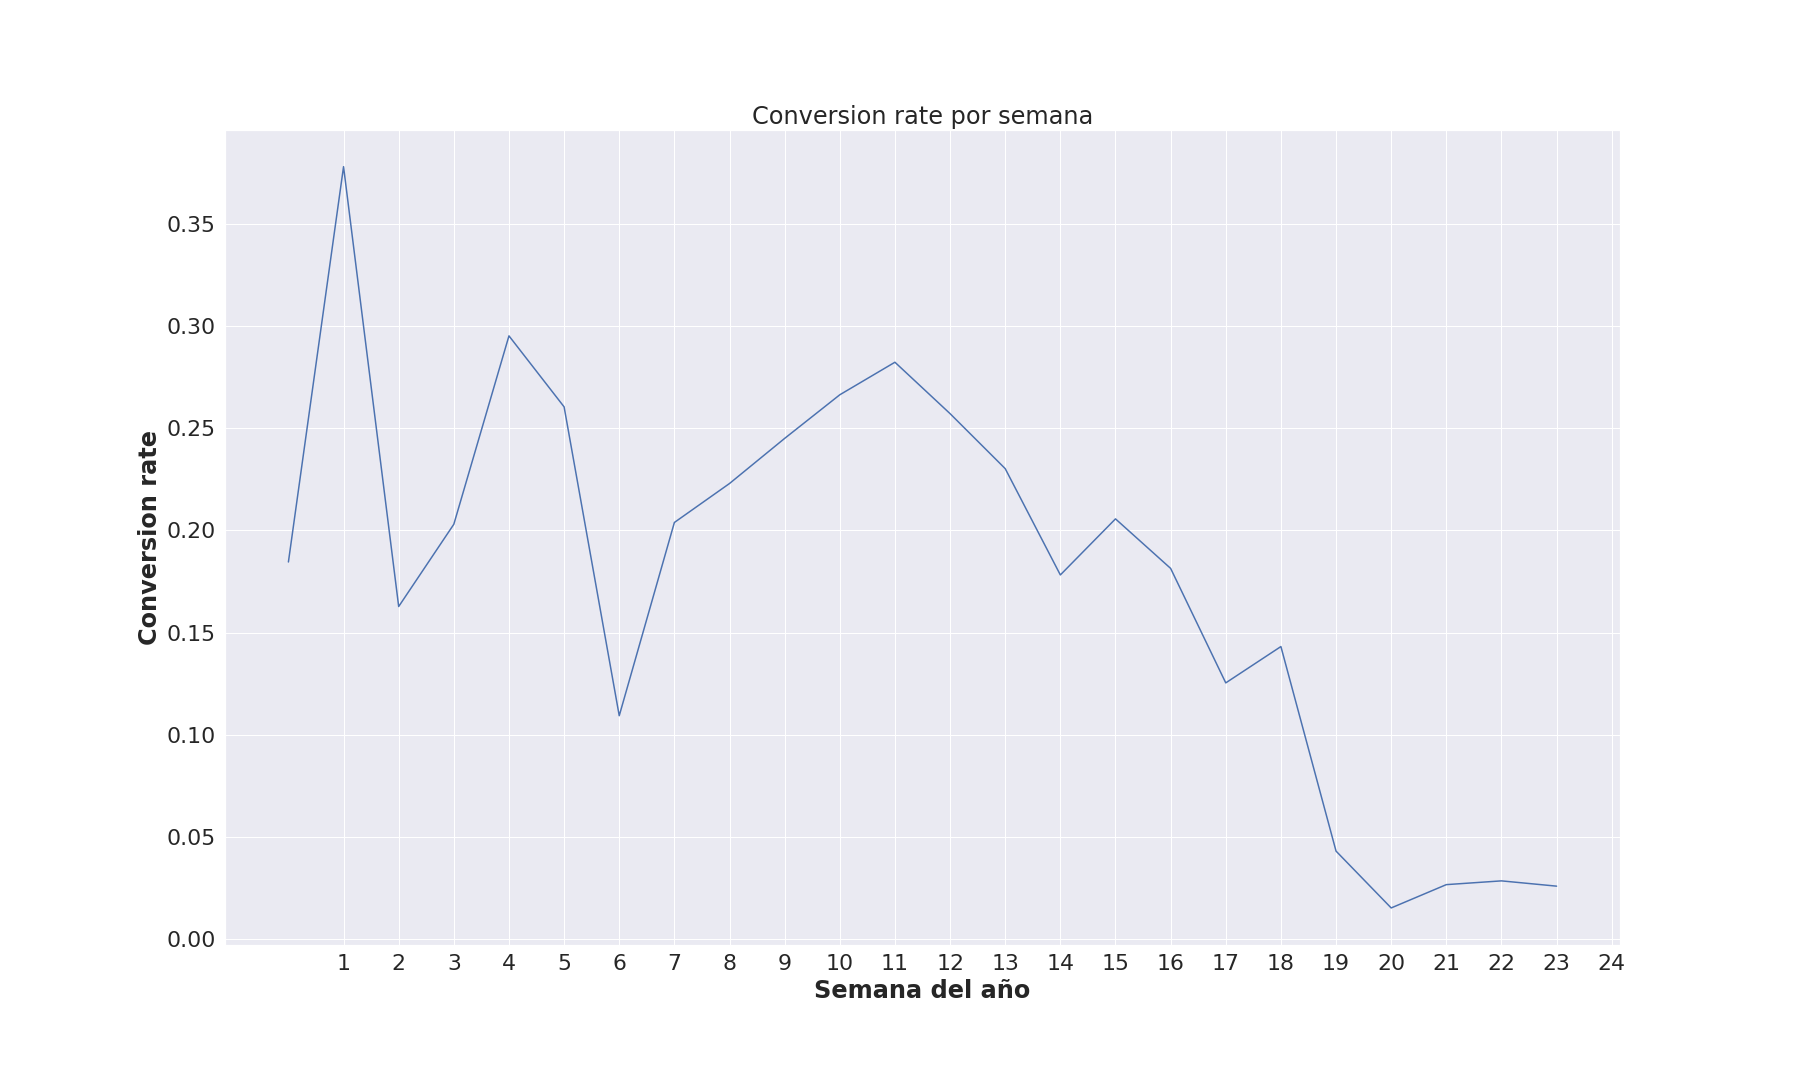
\includegraphics[width=1.2\textwidth]{figures/010-conversion_rate_semana-lineplot.png}}
	\caption{Tasa de conversión a lo largo de las semanas del año}
	\label{fig:conversionrate}
\end{figure}

Las mayores tasas de conversiones se registran en las semanas 1,4 y 11, es decir, enero y marzo. Para observar mejor este fenómeno se realiza otro gráfico (\ref{fig:conversionratemonthly}) que muestre la evolución de la tasa de conversión a lo largo de los meses. 

\begin{figure}[!h]
	\makebox[\textwidth][c]{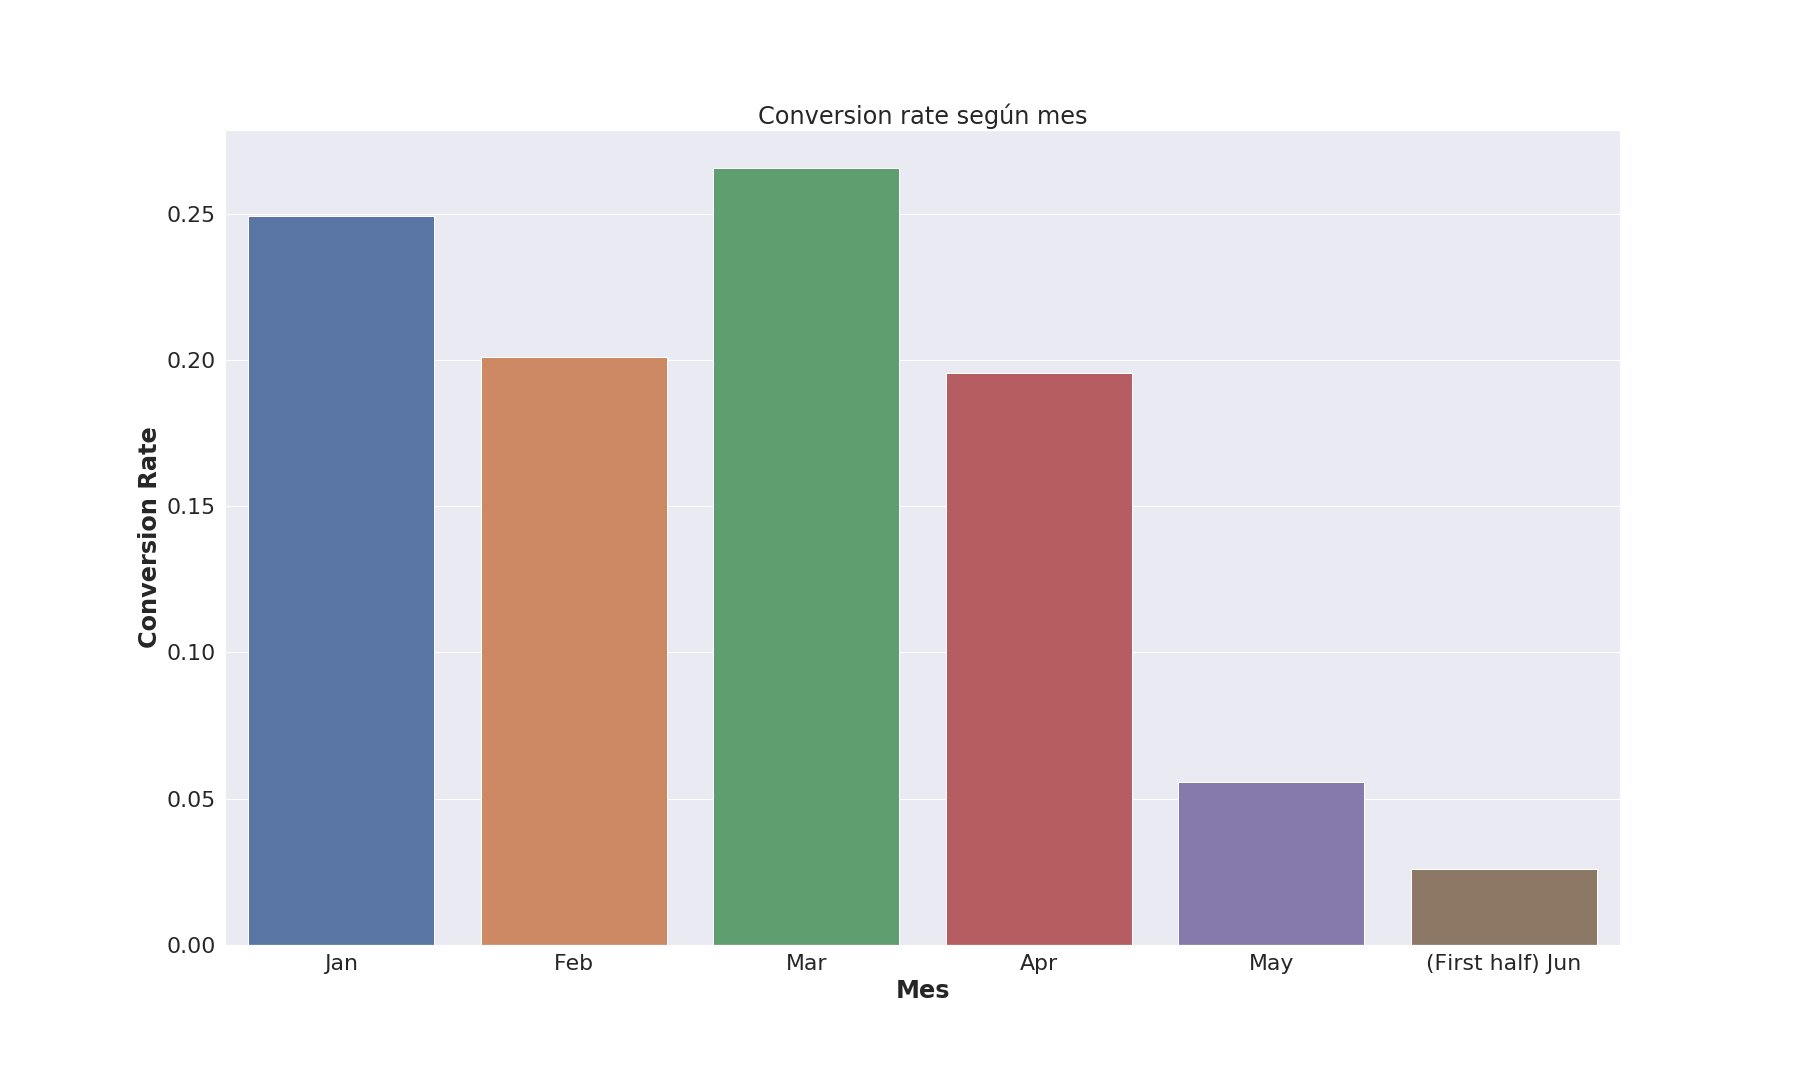
\includegraphics[width=1.2\textwidth]{figures/011-conversion_rate_mes-barplot.png}}
	\caption{Tasa de conversión a lo largo de los meses del año}
	\label{fig:conversionratemonthly}
\end{figure}

Se refuerza la teoría de que enero y marzo fueron los meses de mayor tasa de conversión. Así mismo, dicha tasa se mantiene estable por 4 meses para luego tener una baja en los meses de mayo y junio. Más adelante se analizarán estos dos meses en profundidad.

\subsection{Frecuencia de eventos}

Se analiza qué tipo de evento es el más frecuente en el dataset. Para ello se grafica la cantidad registrada de eventos en función de los distintos tipos de eventos.

\begin{figure}[!h]
	\makebox[\textwidth][c]{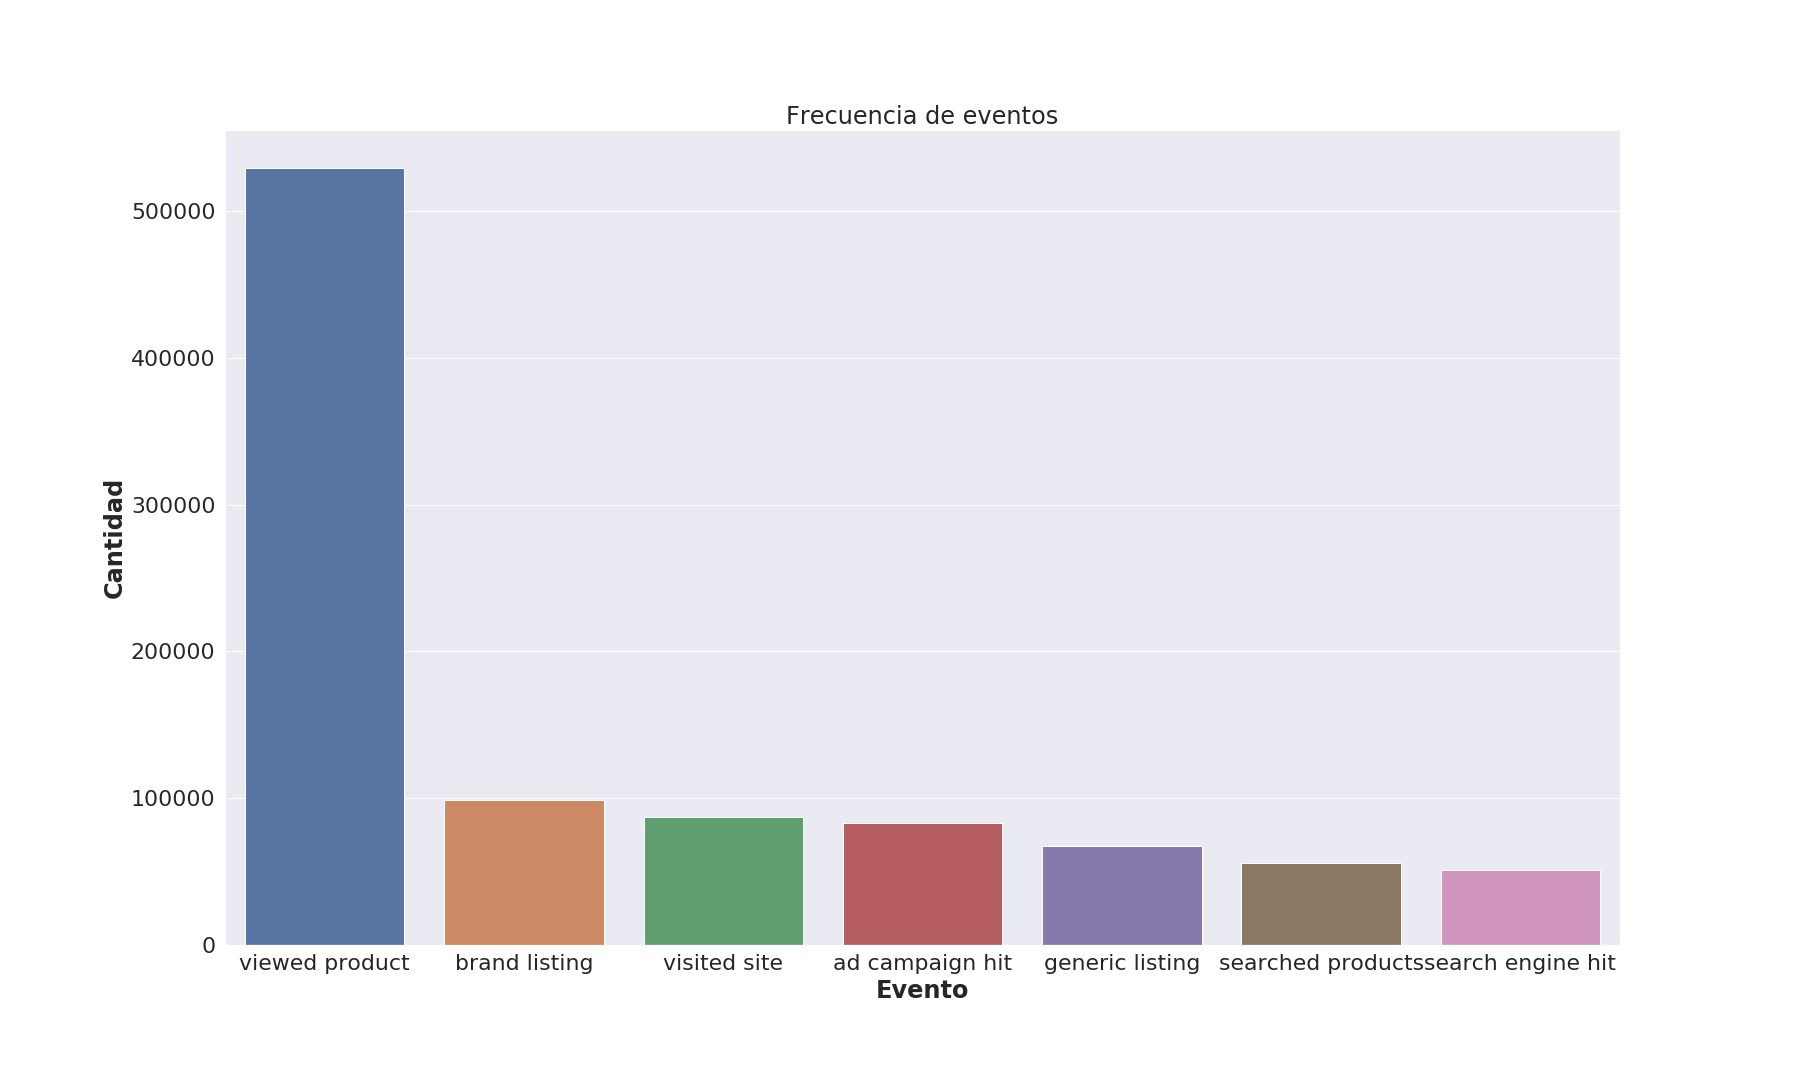
\includegraphics[width=1.2\textwidth]{figures/02-eventos-barplot.png}}
	\caption{Frecuencia de eventos}
	\label{fig:freqeventos}
\end{figure}

Se observa en el gráfico \ref{fig:freqeventos} que la mayor cantidad de eventos se relacionan a la vista de un producto, lo cual era previsible ya que Trocafone es una plataforma de e-commerce y ver productos constituye su principal función como sitio.

\subsection{Evolución de los eventos a través del tiempo}

\subsubsection{Tráfico del sitio de acuerdo al mes y al día}

Otro aspecto a analizar es la cantidad de eventos producidos en cada día de la semana y del mes. Se busca detectar si se mantiene algún comportamiento específico a lo largo de los meses o si la cantidad de eventos registrada depende de algún factor temporal. Un patron esperado a encontrar es el de si hay más visitas o compras de celular en las primeras semanas del mes, lo cual coincidiría con el pago de sueldos mensuales.

\begin{figure}[!h]
	\makebox[\textwidth][c]{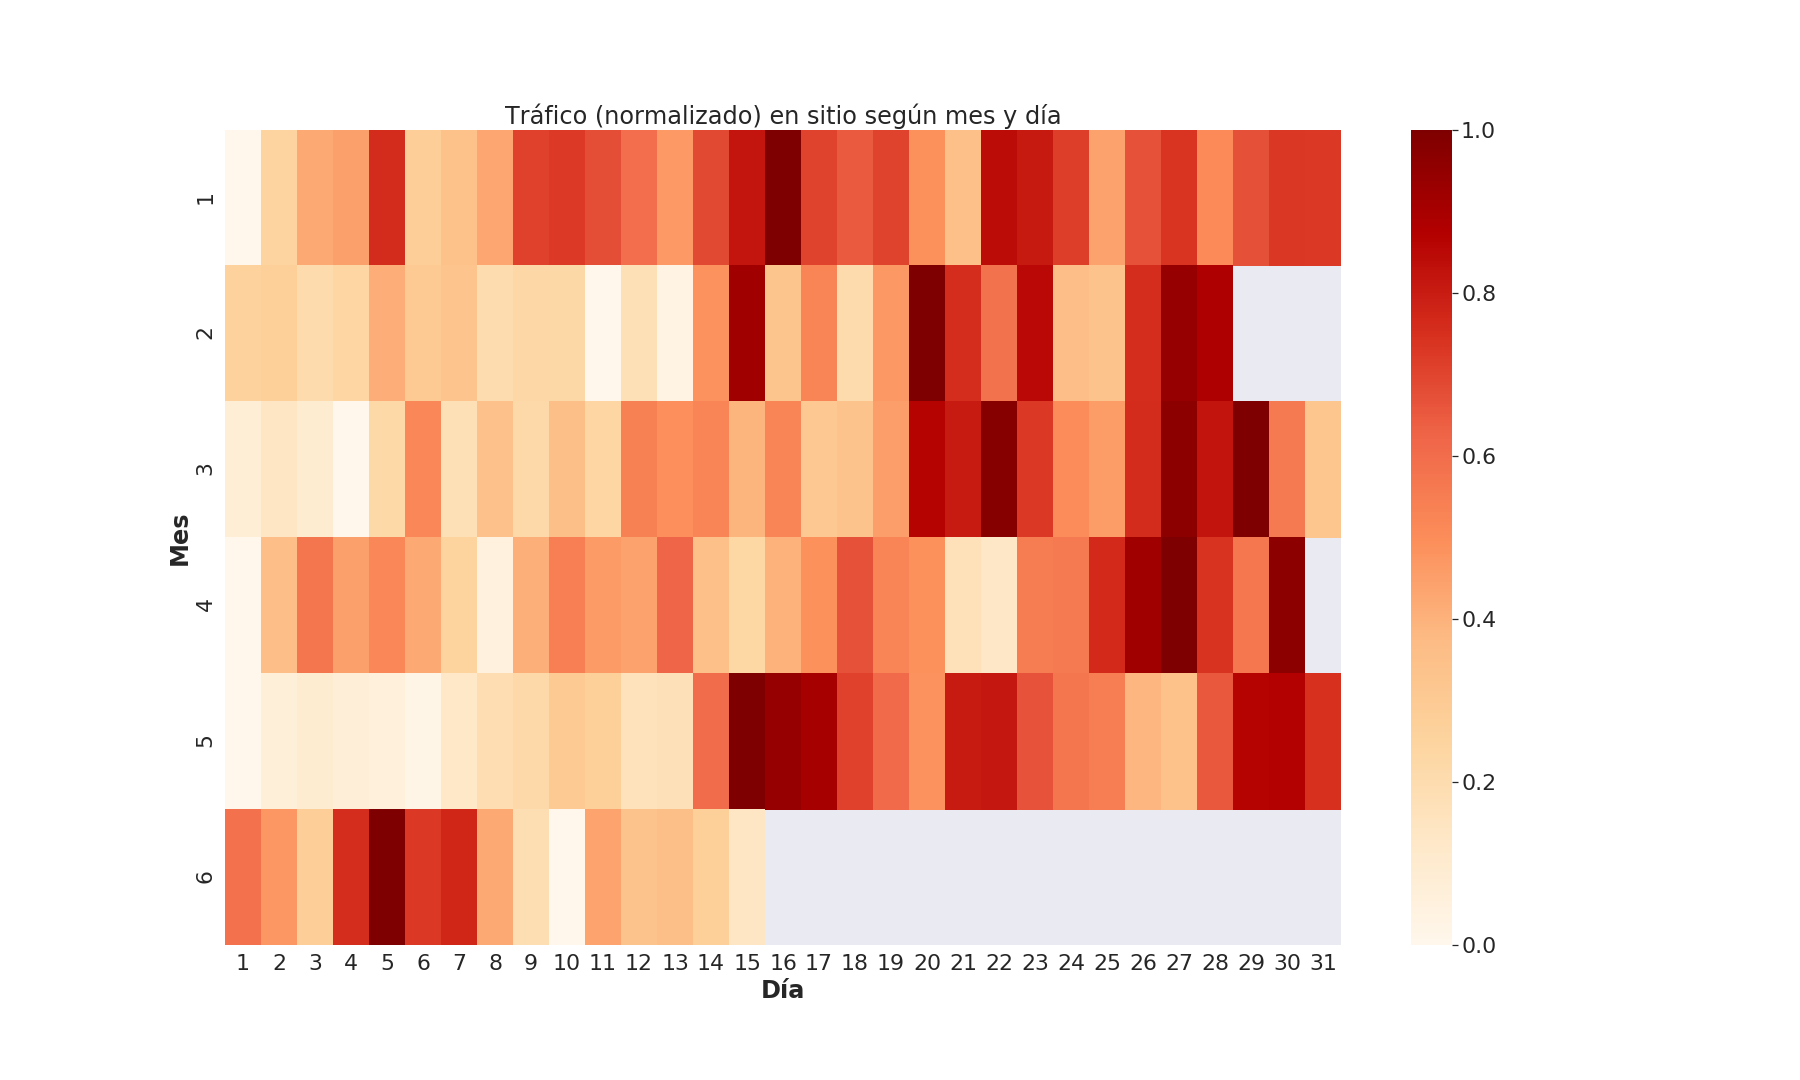
\includegraphics[width=1.2\textwidth]{figures/030-eventos_segun_mes-heatmap.png}}
	\caption{Eventos segun mes y día}
	\label{fig:mesdiasnormalizado}
\end{figure}

Para realizar este gráfico los datos fueron normalizados para evitar llegar a la conclusión que el mes con una mayor cantidad de eventos es el mes con más eventos por díaen totaote{Lo cual sería un error muy grave en el análisis, famosamente conocido gracias a la ecuación de de Moivre}. 

Se desprende del gráfico \ref{fig:mesdiasnormalizado} que la cantidad de eventos registrada no presenta ningún comportamiento específico. Se observa que dicha cantidad aumenta en la segunda quincena de cada mes pero se considera que la diferencia con el resto de los días no tiene la magnitud suficiente como para extraer alguna conclusión fundada. 

\subsubsection{Tráfico del sitio de acuerdo al mes y al día de la semana}

Sin haber encontrado nada acerca del número de día, se buscar ahora analizar si algún día de la semana se registra una mayor cantidad de eventos. 

Se realiza el gráfico \ref{fig:messemanasnormalizado} del mismo estilo que el anterior y se normaliza por las mismas razones.

\begin{figure}[!h]
	\makebox[\textwidth][c]{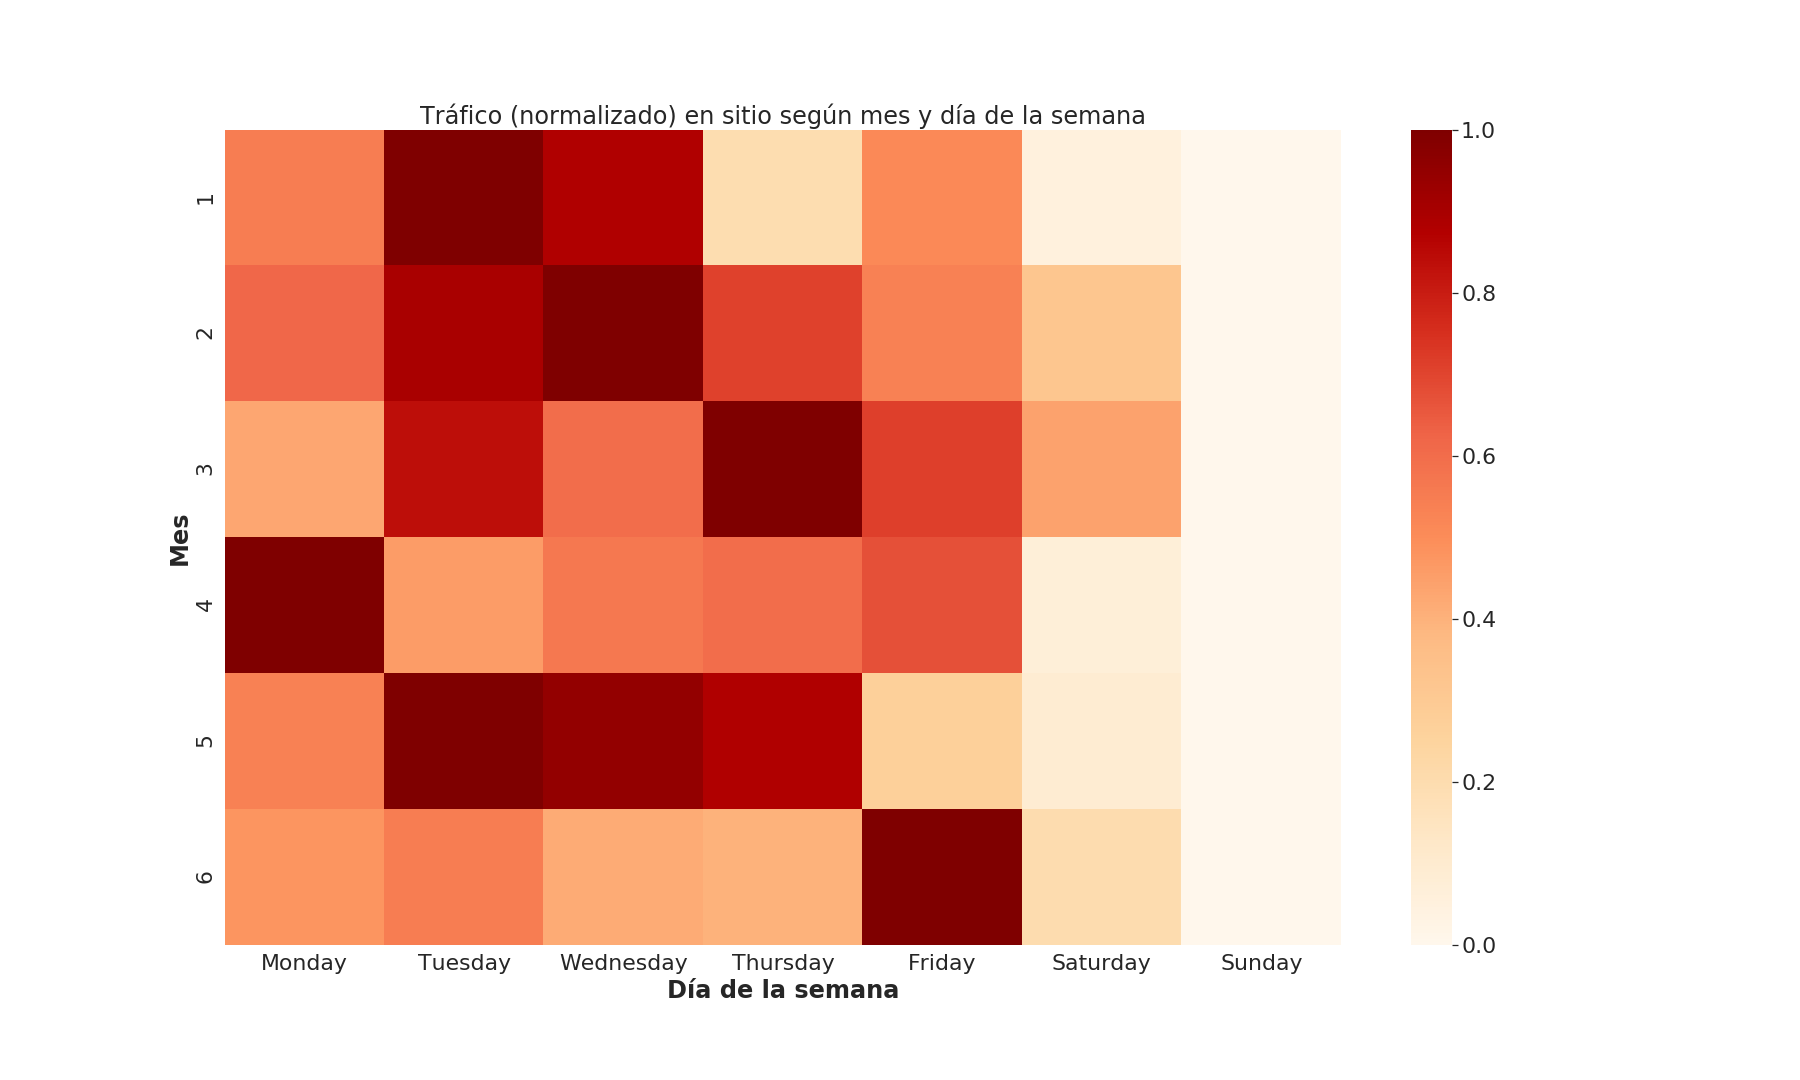
\includegraphics[width=1.2\textwidth]{figures/031-eventos_segun_dow-heatmap.png}}
	\caption{Eventos segun mes y día}
	\label{fig:messemanasnormalizado}
\end{figure}

Es notable que durante los días hábiles de la semana el tráfico es mucho mayor que al fin de semana. Esto puede deberse a que los fines de semana suelen ser días de descanso, donde la gente puede no estar pensando en realizar una compra, además de no poder retirarla. En la semana aumenta el tráfico debido a que el envío o el retiro del celular puede realizarse en el momento.

\subsubsection{Tráfico del sitio según mes}

Habiendo analizado las semanas, ahora se hace un enfoque más global, buscando patrones de tráfico según el mes. En este apartado se busca analizar si en algún mes se registró una mayor cantidad de eventos o si la distribución de las visitas fue uniforme a lo largo del tiempo.

\begin{figure}[!h]
	\makebox[\textwidth][c]{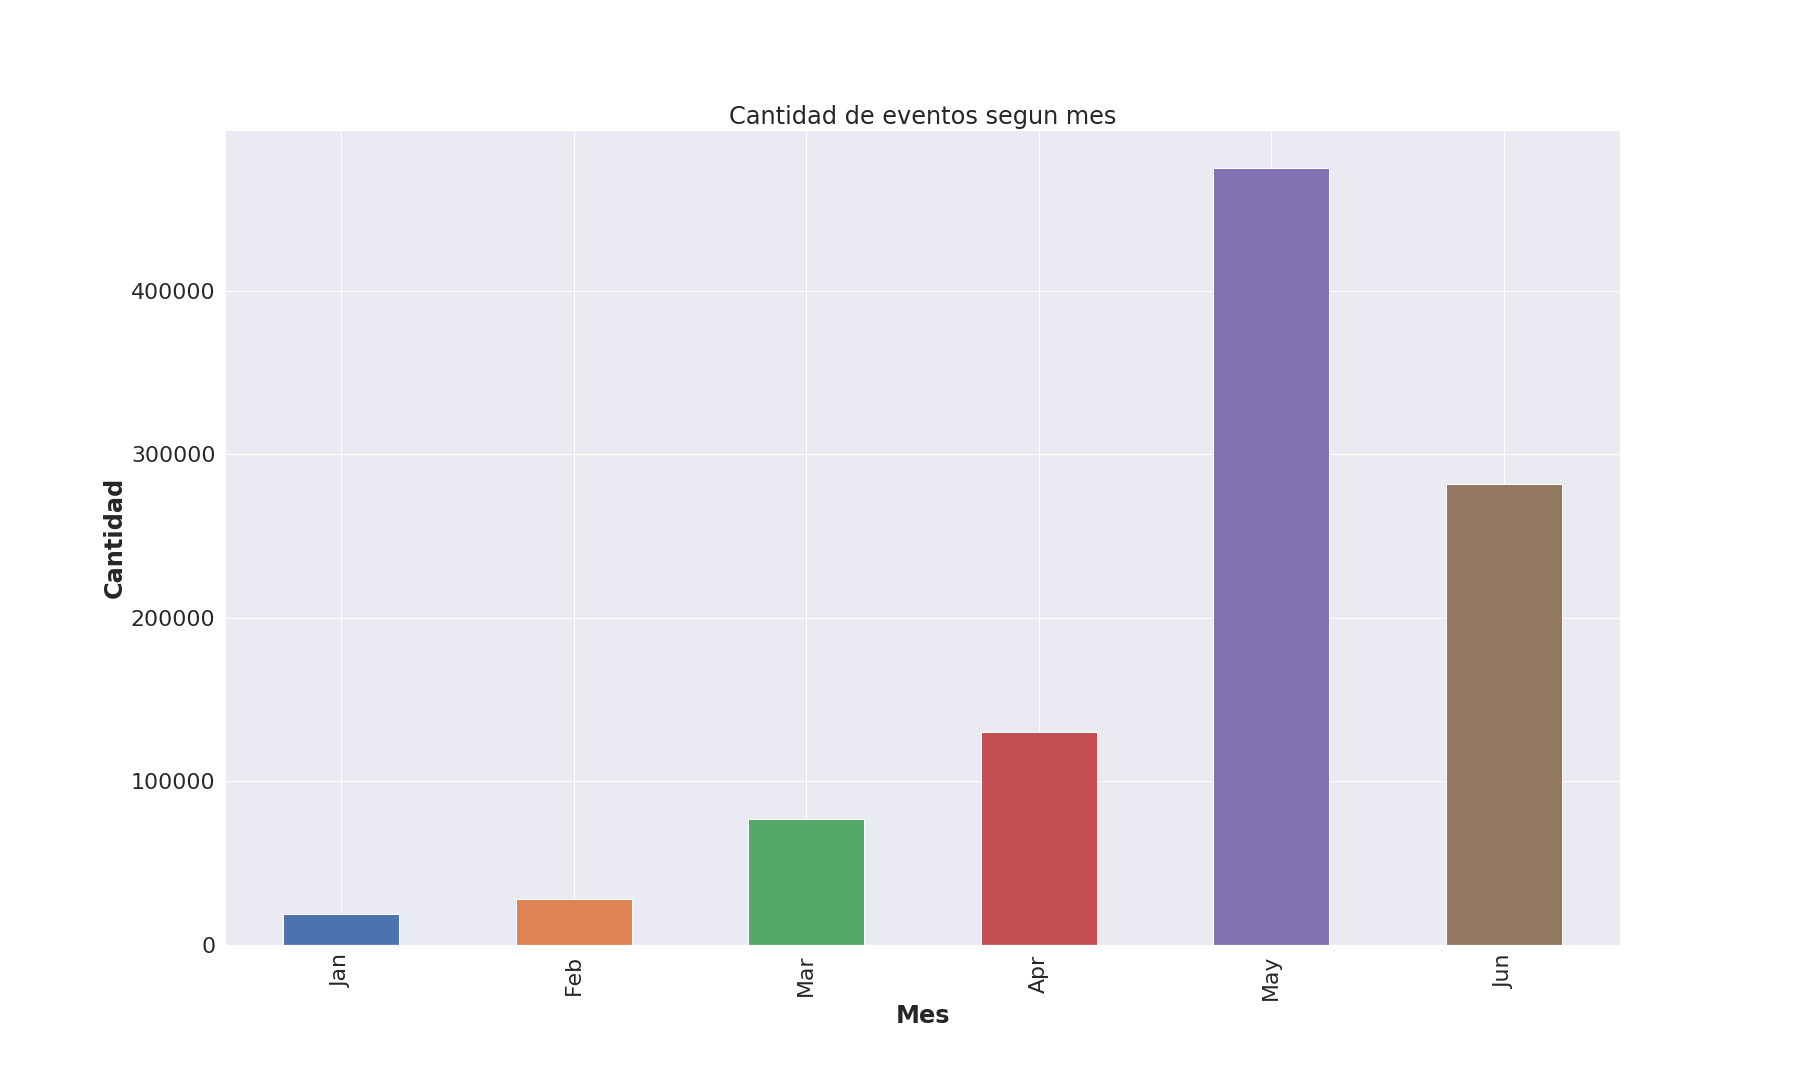
\includegraphics[width=1.2\textwidth]{figures/032-eventos_segun_mes-barplot.png}}
	\caption{Eventos segun mes}
	\label{fig:mes}
\end{figure}

El gráfico \ref{fig:mes} muestra que en los meses de mayo y junio se registró una cantidad notablemente mayor de eventos. Este resultado llama la atención por lo que se analiza en mayor profundidad en la próxima sección. Es importante destacar que esta evolución es inversa a la de la tasa de conversión. De estos dos datos se concluye que en mayo si bien no hubo tantas ventas, sí aumentó mucho la cantidad de eventos. 

\subsubsection{¿Por qué mayo y junio registran una mayor cantidad de eventos?}

Para tratar de encontrar una respuesta a esta pregunta se centra el análisis en estos meses y se estudian los tres eventos principales del dataset: \texttt{conversion}, \texttt{checkout} y \texttt{viewed products}. Es pertinente recordar que no se dispone de todos los datos del mes de junio, sino solo de los primeros 16 días.

\begin{figure}[!h]
	\makebox[\textwidth][c]{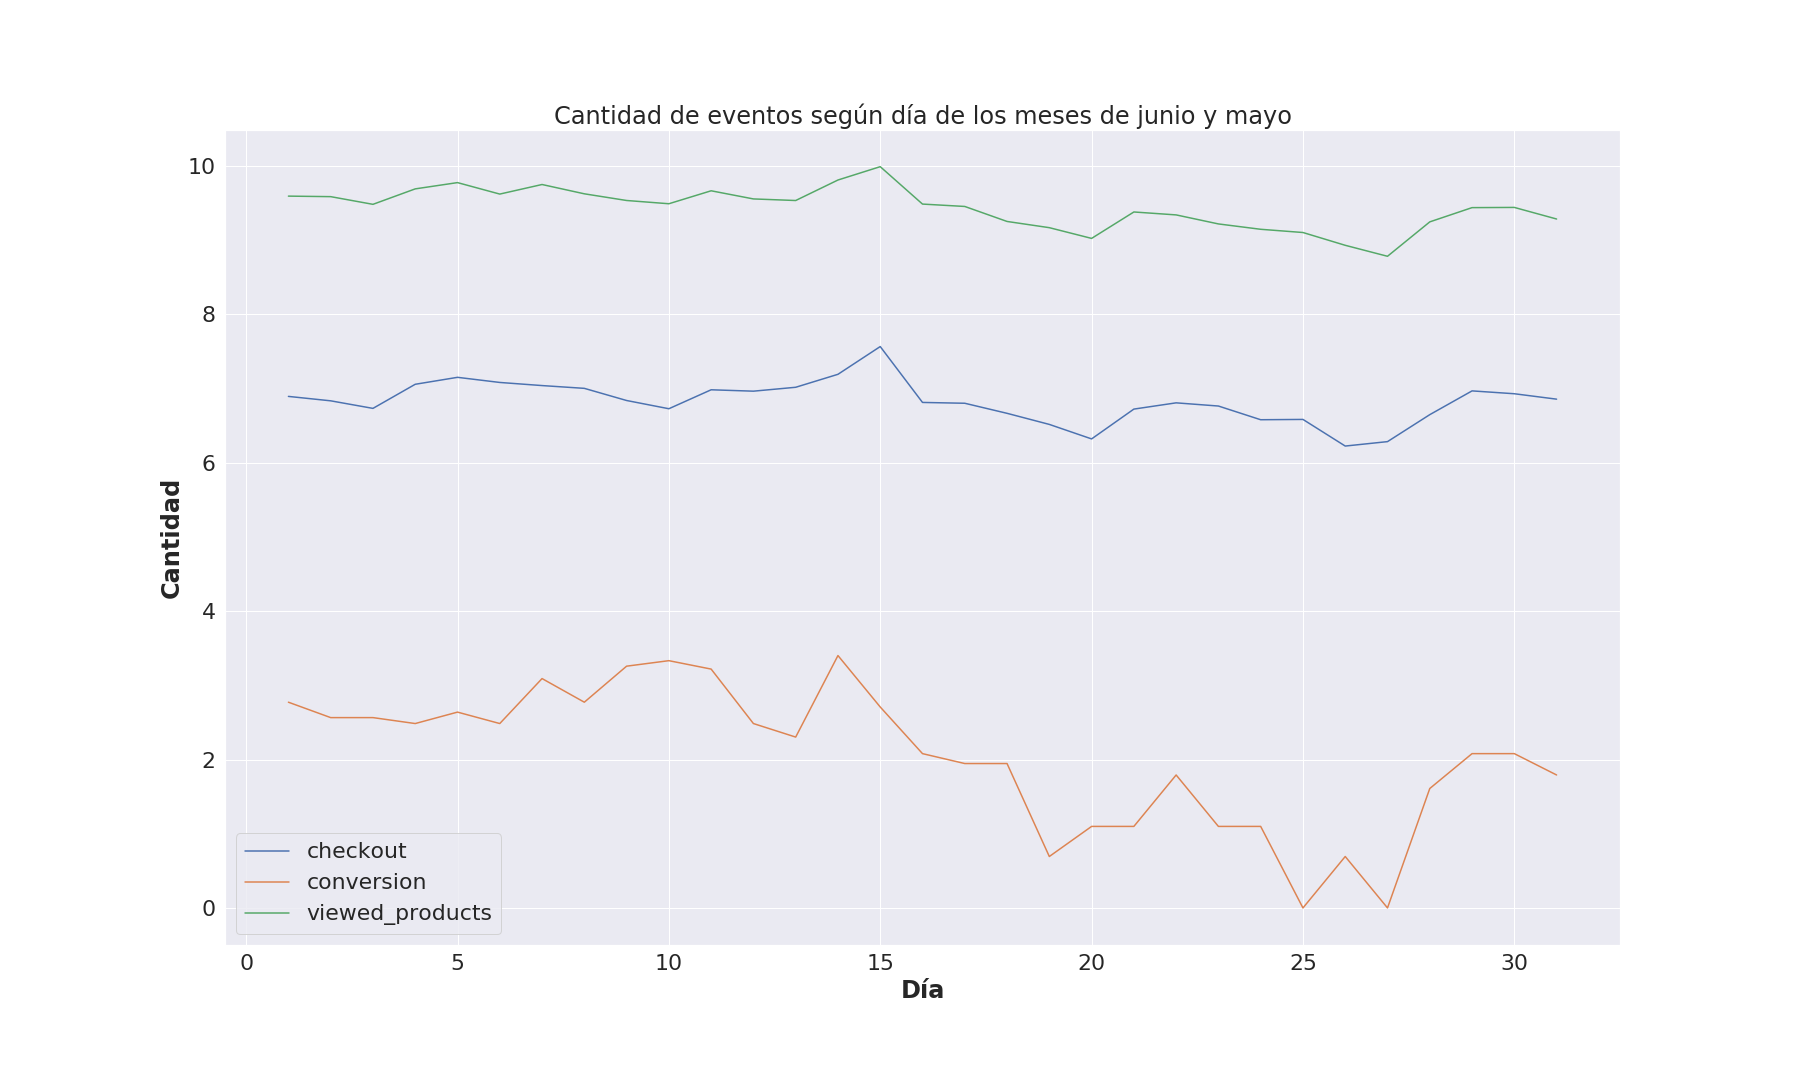
\includegraphics[width=1.2\textwidth]{figures/033-eventos_mayo_junio_lineplot.png}}
	\caption{Conversiones, checkouts y viewed products a lo largo de los días del mes de mayo y junio en éscala logarítmica}
	\label{fig:mayojunio}
\end{figure}

Como se ve en la figura \ref{fig:mayojunio}, los tres eventos presentan su máximo alrededor de los días 14 a 16. Como Trocafone es del país de Brasil y el mayor tráfico proviene de allí (lo cual será verificado posteriormente) se infiere que puede deberse a alguna promoción lanzada en la plataforma o en el mismo país. Esto no puede concluirse con certeza debido a la falta de información en internet y en la plataforma de promociones pasadas.

\subsubsection{Hora de mayor cantidad de conversiones y checkouts}

En un intento de encontrar un patrón por parte de los clientes se grafica la cantidad de conversiones y de checkouts en función de las horas del día. Se busca determinar la hora en la que ambas confluyan en su máximo para analizar el motivo por el que dicha hora registra mayor tráfico.

\begin{figure}[!h]
	\centering
	\begin{minipage}[b]{0.4\textwidth}
		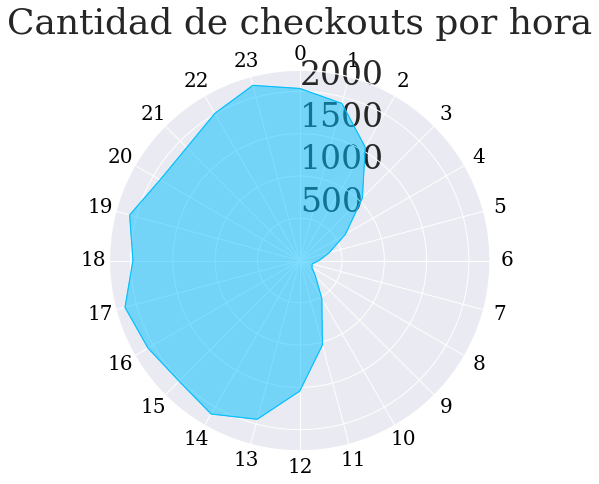
\includegraphics[width=6cm,height=6cm,keepaspectratio]{figures/041-hours-checkout-radarchart.png}
		\caption{Conversiones a lo largo de las horas del día}
	\end{minipage}
	\hfill
	\begin{minipage}[b]{0.4\textwidth}
		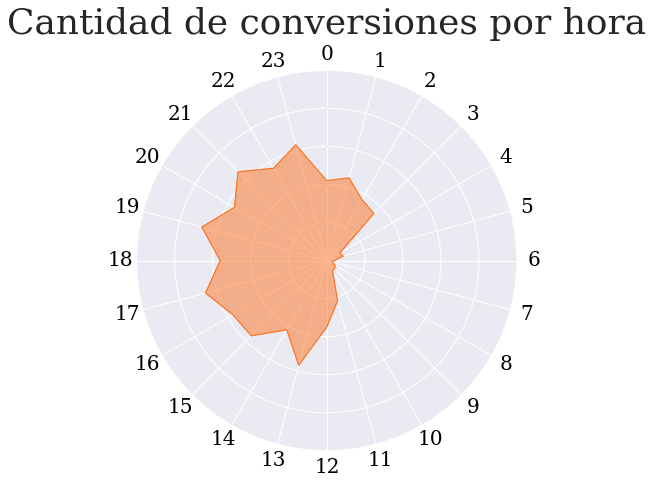
\includegraphics[width=6cm,height=6cm,keepaspectratio]{figures/040-hours-conversion-radarchart.png}
		\caption{Conversiones a lo largo de las horas del día}
	\end{minipage}
\end{figure}

Se observa que ambos gráficos confluyen en su máximo a las 19 hs. Esto puede significar que la mayoría de los usuarios deciden realizar conversiones o checkouts cuando vuelven del trabajo o están finalizando su día. La diferencia entre ambos gráficos es que la cantidad de checkouts realizados se mantiene relativamente constante en las segundas 12 hs del día mientras que las conversiones son mucho menores y presentan picos más marcados en los horarios de la tarde-noche. 

\subsection{Distribución de la cantidad de eventos producidos por usuario}

Se propone analizar la cantidad de eventos producidos por usuario. Se confecciona un gráfico tomando algunas salvedades que son necesarias para obtener una buena visualización:

\begin{itemize}
	\item Se trunca el eje y a un valor determinado para una mejor observación de los \textit{box}
	\item En los eventos donde no se registran datos para usuarios se coloca el valor promedio.
\end{itemize}


\begin{figure}[!h]
	\makebox[\textwidth][c]{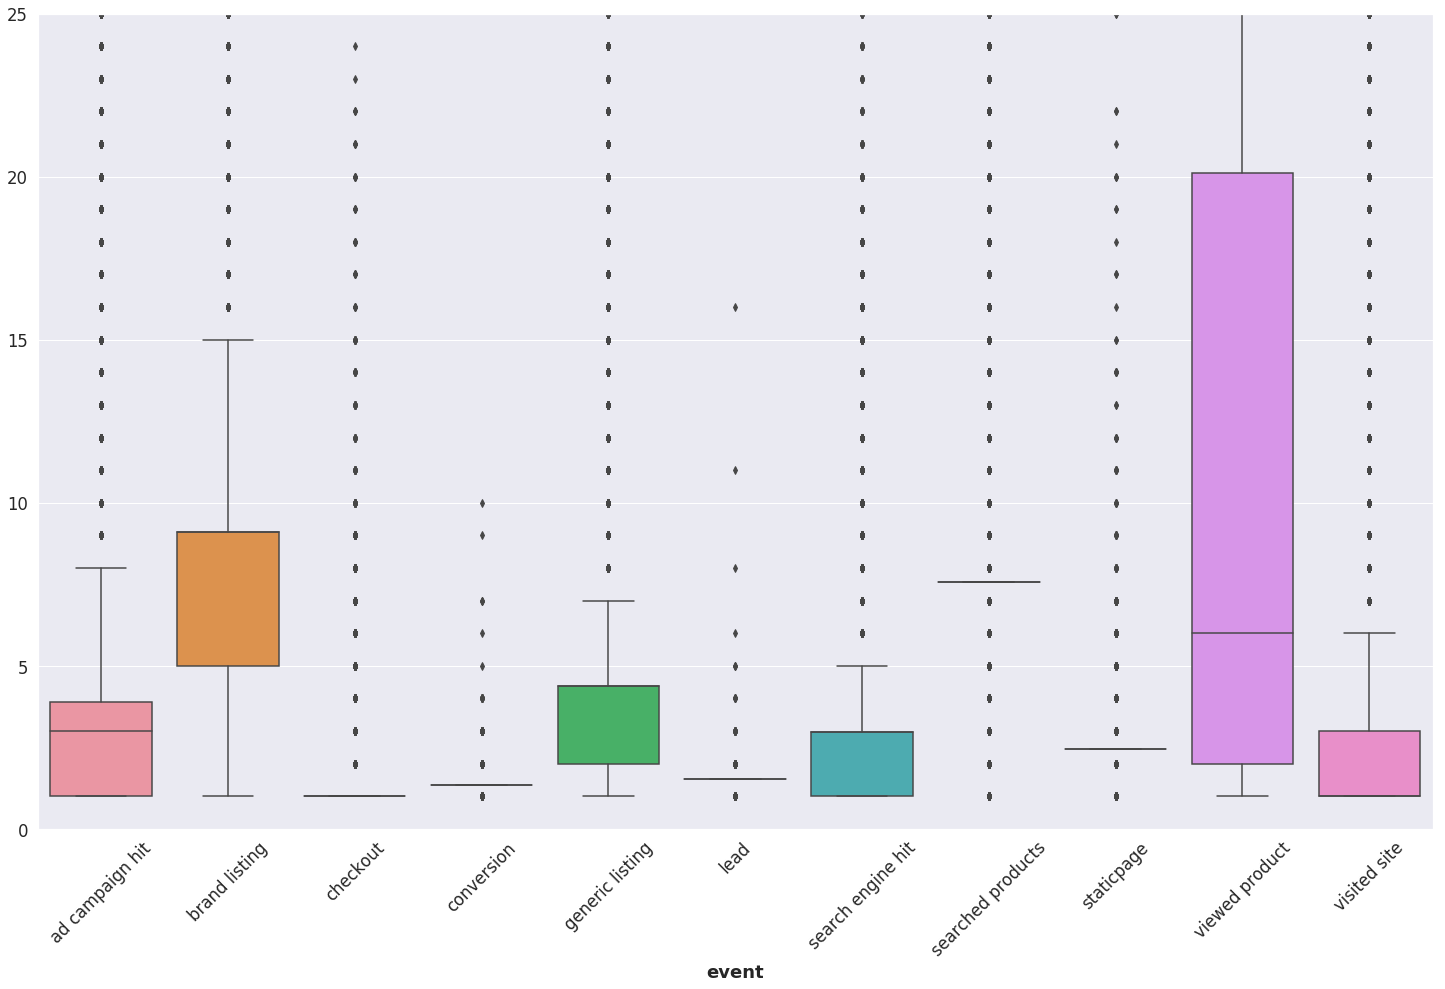
\includegraphics[width=1.2\textwidth]{figures/191-usuarios_eventos_truncado-boxplot.png}}
	\caption{Distribución de los eventos agrupados por usuario}
	\label{fig:boxplot}
\end{figure}

Se puede observar en el gráfico \ref{fig:boxplot} que los usuarios suelen más comúnmente ver los productos antes que comprarlos, algo que podía predecirse anteriormente. Lo que puede resultar llamativo es que la cantidad de usuarios que ven productos es mayor a los que los buscan, pero esto se puede explicar por el hecho de que en una búsqueda pueden verse varios productos a la vez y eso cuenta como un solo evento. En cambio, ante el evento \texttt{viewed products} cada vista de producto se contabiliza como un evento.

\section{Análisis geográfico}

En este apartado se busca analizar las ciudades, países y regiones de dónde provienen los distintos tipos de eventos. Trocafone es una empresa que inició en Brasil y expandió sus comercios a Argentina en el 2015, por lo que se deduce que probablemente Brasil sea la zona de mayor influencia en los eventos.

\subsection{Países que registran mayor cantidad de eventos} 

\begin{figure}[!h]
	\makebox[\textwidth][c]{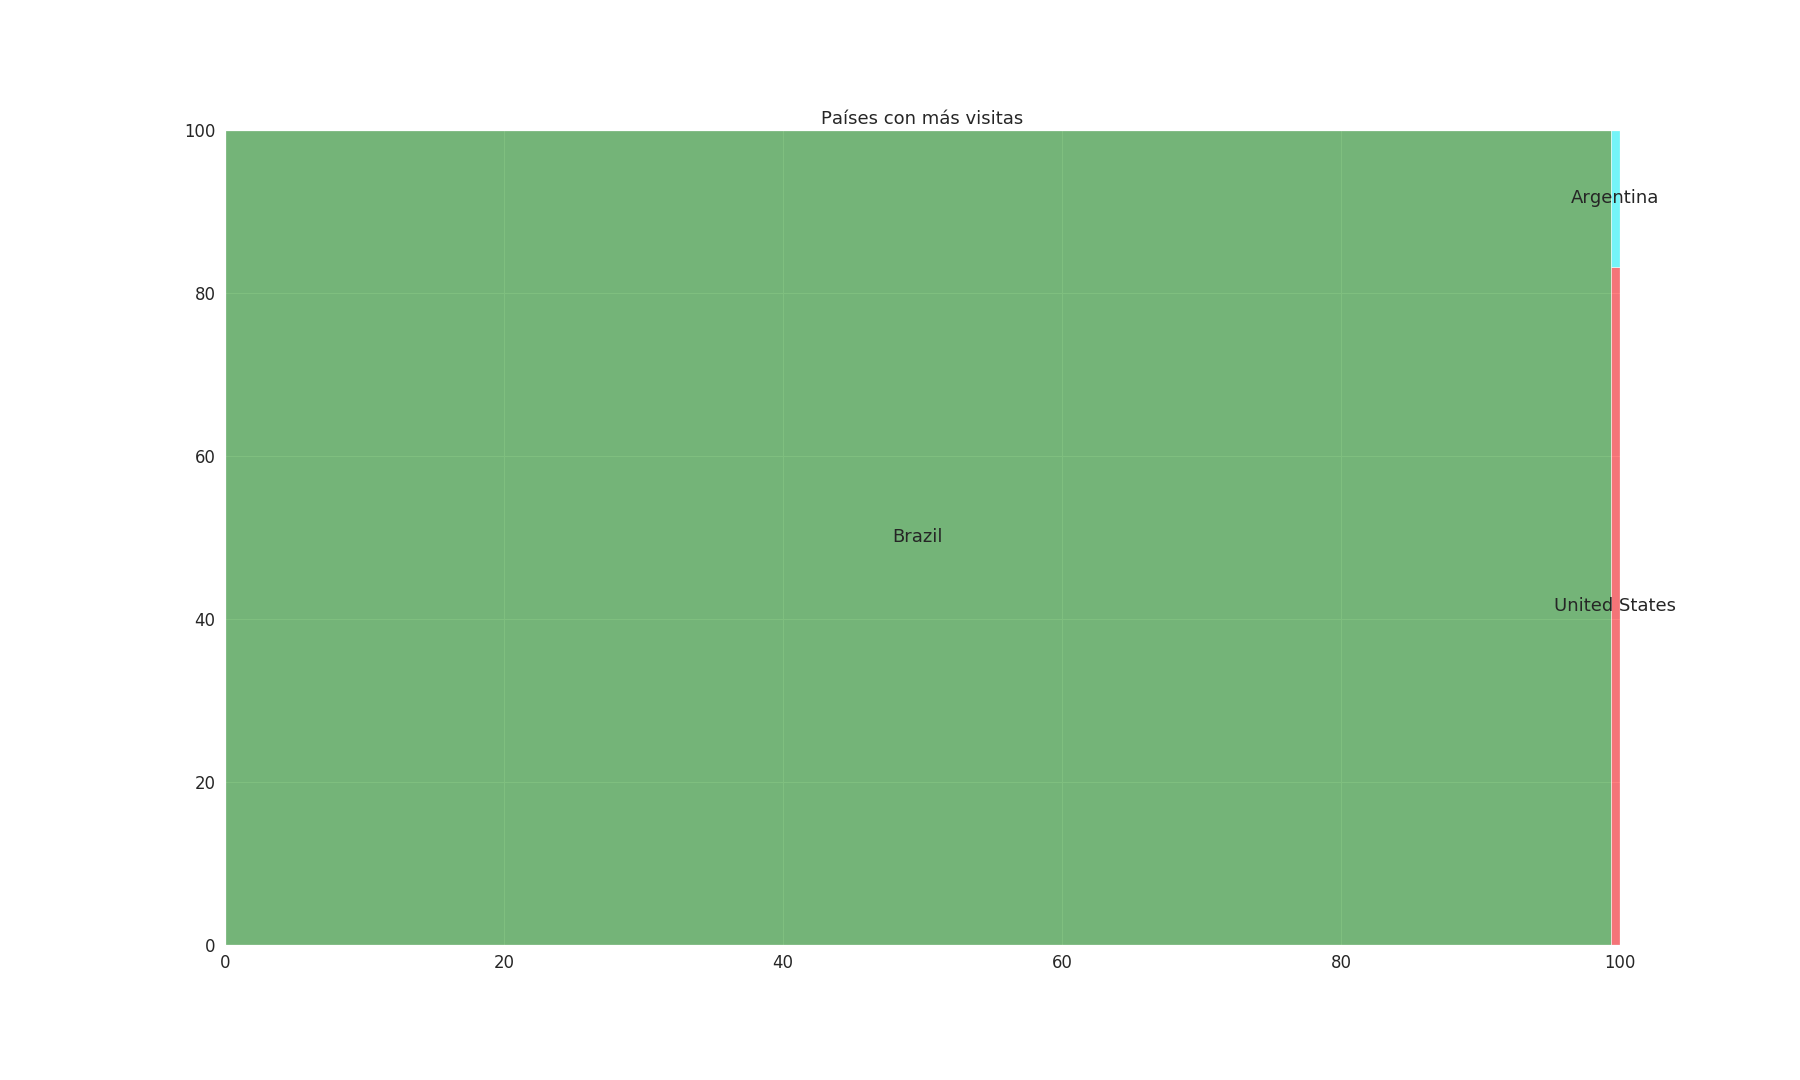
\includegraphics[width=1.2\textwidth]{figures/050-paises_visitas-treemap.png}}
	\caption{Países de mayor tráfico de la página}
	\label{fig:brazilrules}
\end{figure}

\begin{figure}[!h]
	\makebox[\textwidth][c]{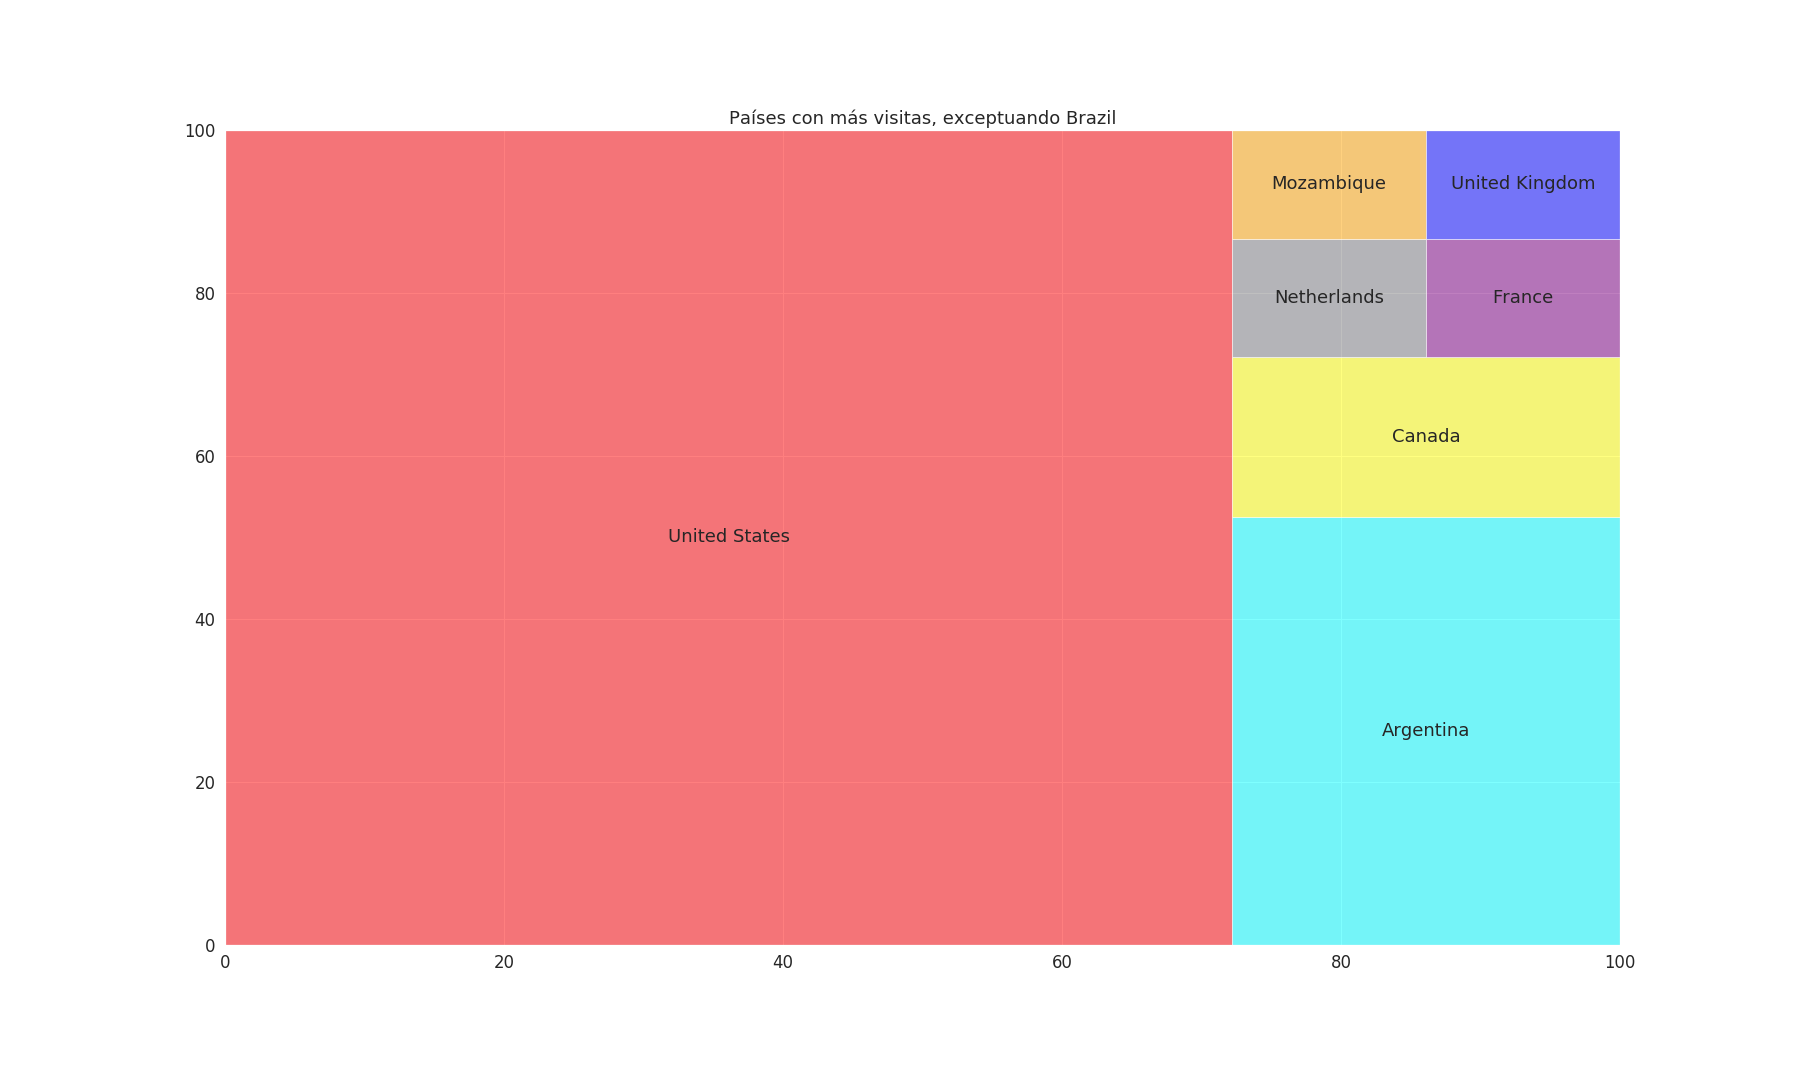
\includegraphics[width=1.2\textwidth]{figures/051-paises_visitas_sin_brazil-treemap.png}}
	\caption{Países de mayor tráfico de la página sin contar a Brasil}
	\label{fig:brazilsucks}
\end{figure}

Se corrobora en el gráfico \ref{fig:brazilrules} la teoría inicial de que Brasil sería el país con más visitas, por lo que se procedió a eliminarlo del gráfico, generando el gráfico \ref{fig:brazilsucks}, para poder observar qué otros países intervienen en la página de Trocafone y en qué diferencia de magnitud y orden lo hacen. Estados Unidos supera en una amplia cantidad la influencia en la página a Argentina, a pesar de ser esta una de las sedes de la empresa. Esto puede explicarse debido a que la gran mayoría de los eventos no son conversiones, por lo tanto es factible que cualquier persona de los Estados Unidos busque celulares en la plataforma, sin llegar a registrar un evento de tipo \texttt{checkout} o \texttt{conversión}.

\subsection{Regiones y ciudades de Brasil que registran mayor cantidad de eventos}

Se procede a analizar qué ciudades y regiones de Brasil son las que registran mayor cantidad de eventos. Para ello se grafica las regiones con una mayor cantidad de visitas. Se observa que las tres regiones con la mayor cantidad de eventos (San Pablo, Minas Gerais y Rio de Janeiro) están sobre la costa del sudeste. Para visualizar esto de una mejor manera se realiza un gráfico que muestra las ciudades de Brasil más visitadas y se verifica que la mayoría de los eventos se producen sobre la costa sudeste.

\begin{figure}[!h]
	\makebox[\textwidth][c]{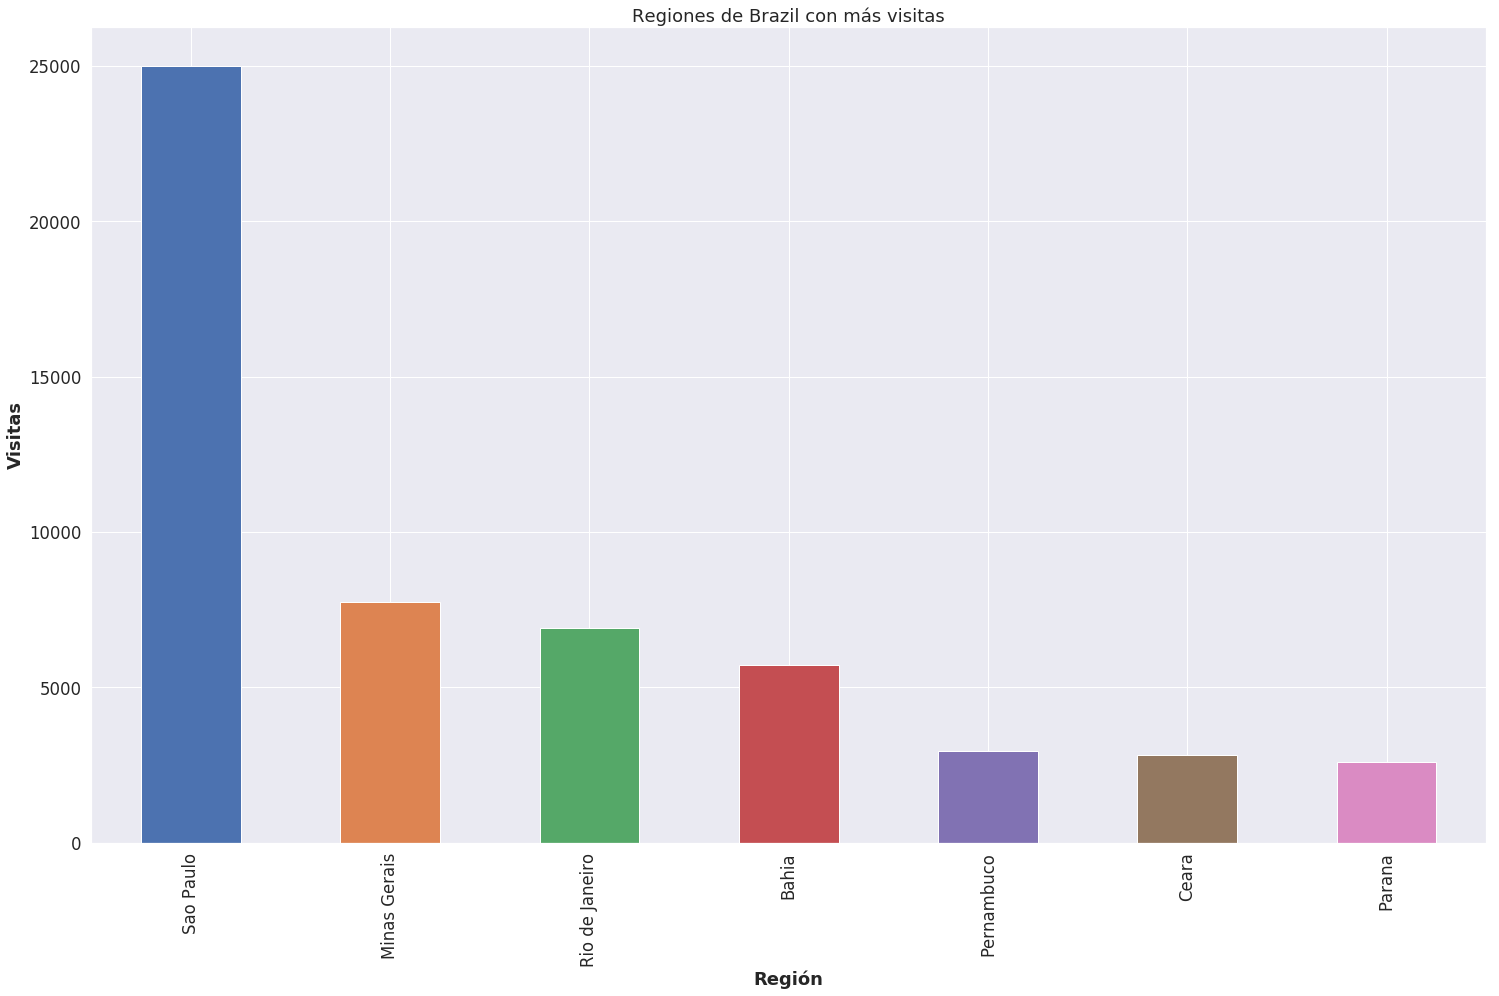
\includegraphics[width=1.2\textwidth]{figures/060-regiones_brazil-barplot.png}}
	\caption{Regiones de Brasil con mayor cantidad de eventos}
	\label{fig:regionsbrasil}
\end{figure}

\begin{figure}[!h]
	\makebox[\textwidth][c]{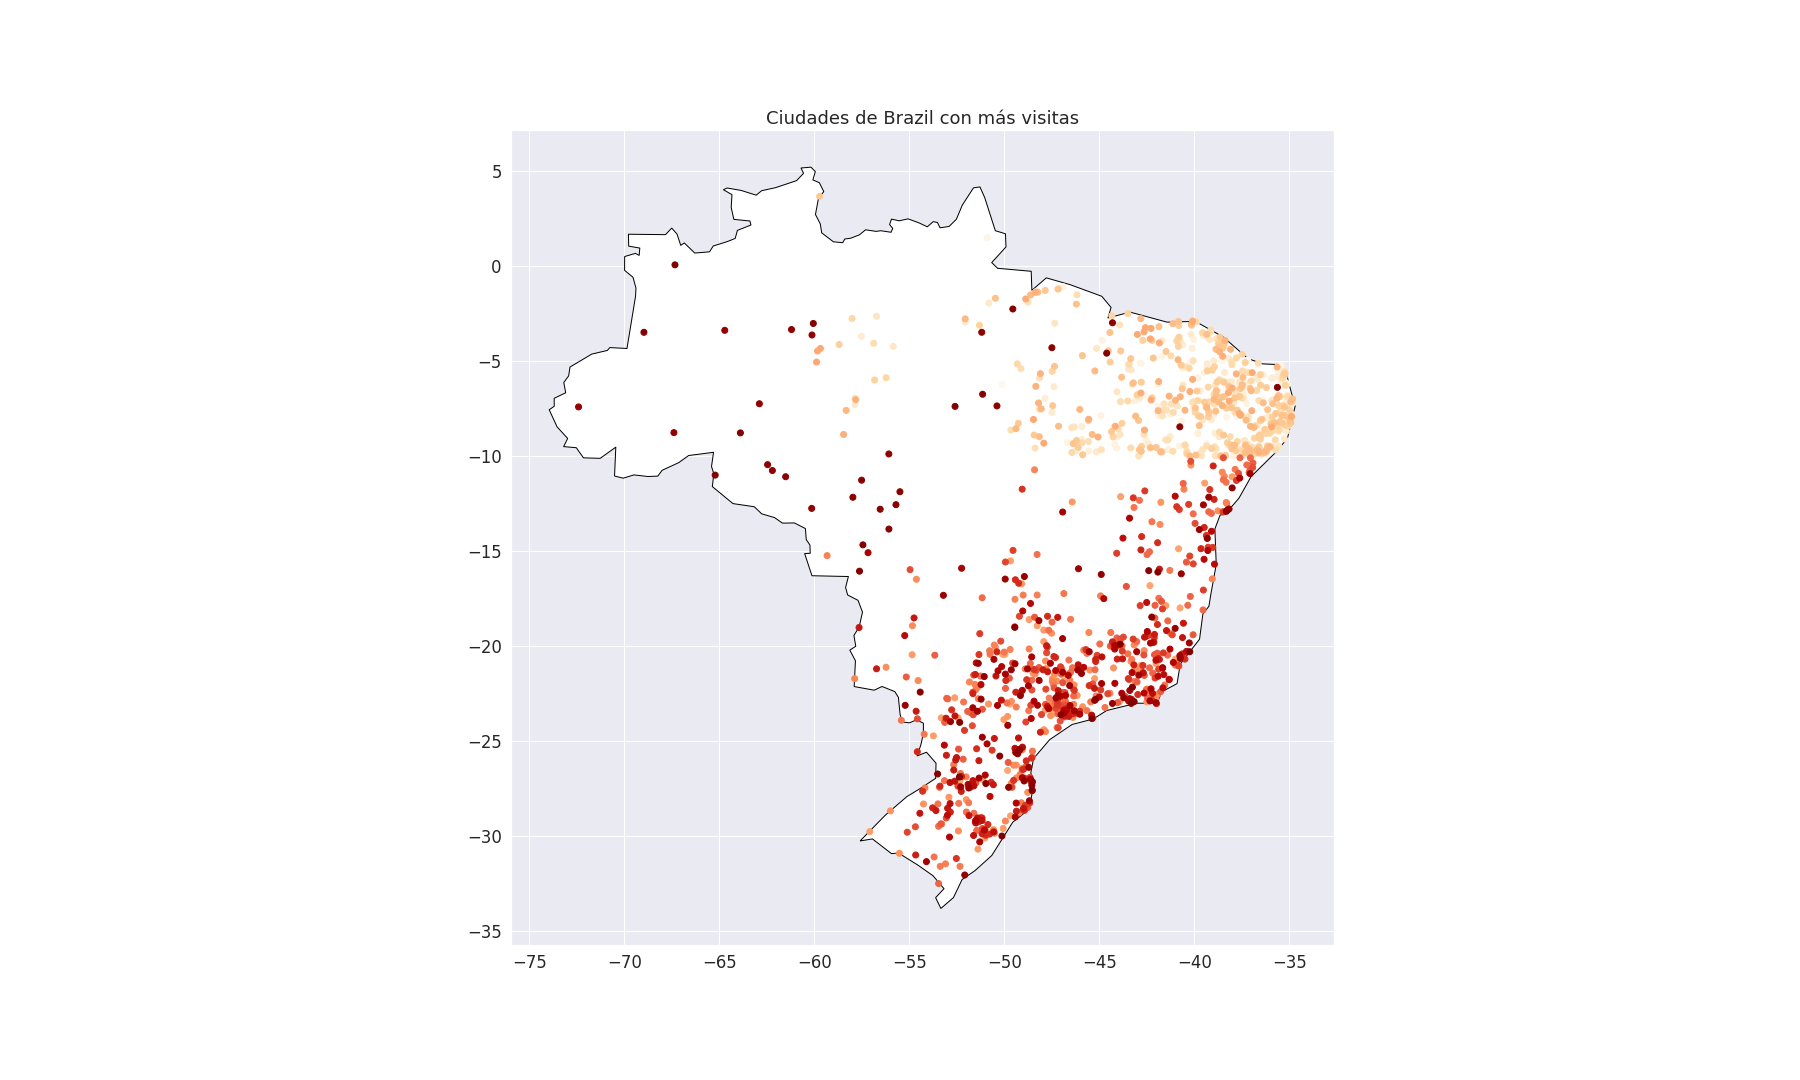
\includegraphics[width=1.2\textwidth]{figures/061-ciudades_brazil-choropleth.png}}
	\caption{Ciudades de Brasil con mayor cantidad de eventos}
	\label{fig:citybrasil}
\end{figure}

Lo que presentan los gráficos \ref{fig:regionsbrasil} y \ref{fig:citybrasil} tiene sentido, considerando que sobre el mayor blanco del gráfico es donde esta la selva brasileña.

\section{Análisis de búsquedas} \label{busq}

La idea de este apartado radica en analizar los términos que buscan los usuarios en la plataforma y así identificar ciertos patrones de búsqueda como por ejemplo cuál es el modelo de celular más buscado. Este análisis se dividirá en dos:

\begin{itemize}
	\item \underline{Términos ingresados en el buscador}: se utiliza la columna \texttt{search\_term} del dataframe.
	\item \underline{Productos buscados en la plataforma}: se utiliza la columna \texttt{event} del dataframe para buscar aquellos eventos que correspondan a \texttt{searched\_product}.
 \end{itemize}

\subsection{Términos ingresados en el buscador}

Se realiza un gráfico para visualizar a grandes rasgos los términos más buscados por los usuarios. Se busca tener una idea aproximada de los modelos de celular más requeridos o deseados por los usuarios. Figuran en el gráfico los términos que fueron buscados como mínimo 300 veces, un número impuesto para fijar un límite mínimo de búsquedas para que un término sea considerado de los más buscados. De no fijar este límite el gráfico estaría sobrecargado y sería difícil de interpretar.

\begin{figure}[!h]
	\makebox[\textwidth][c]{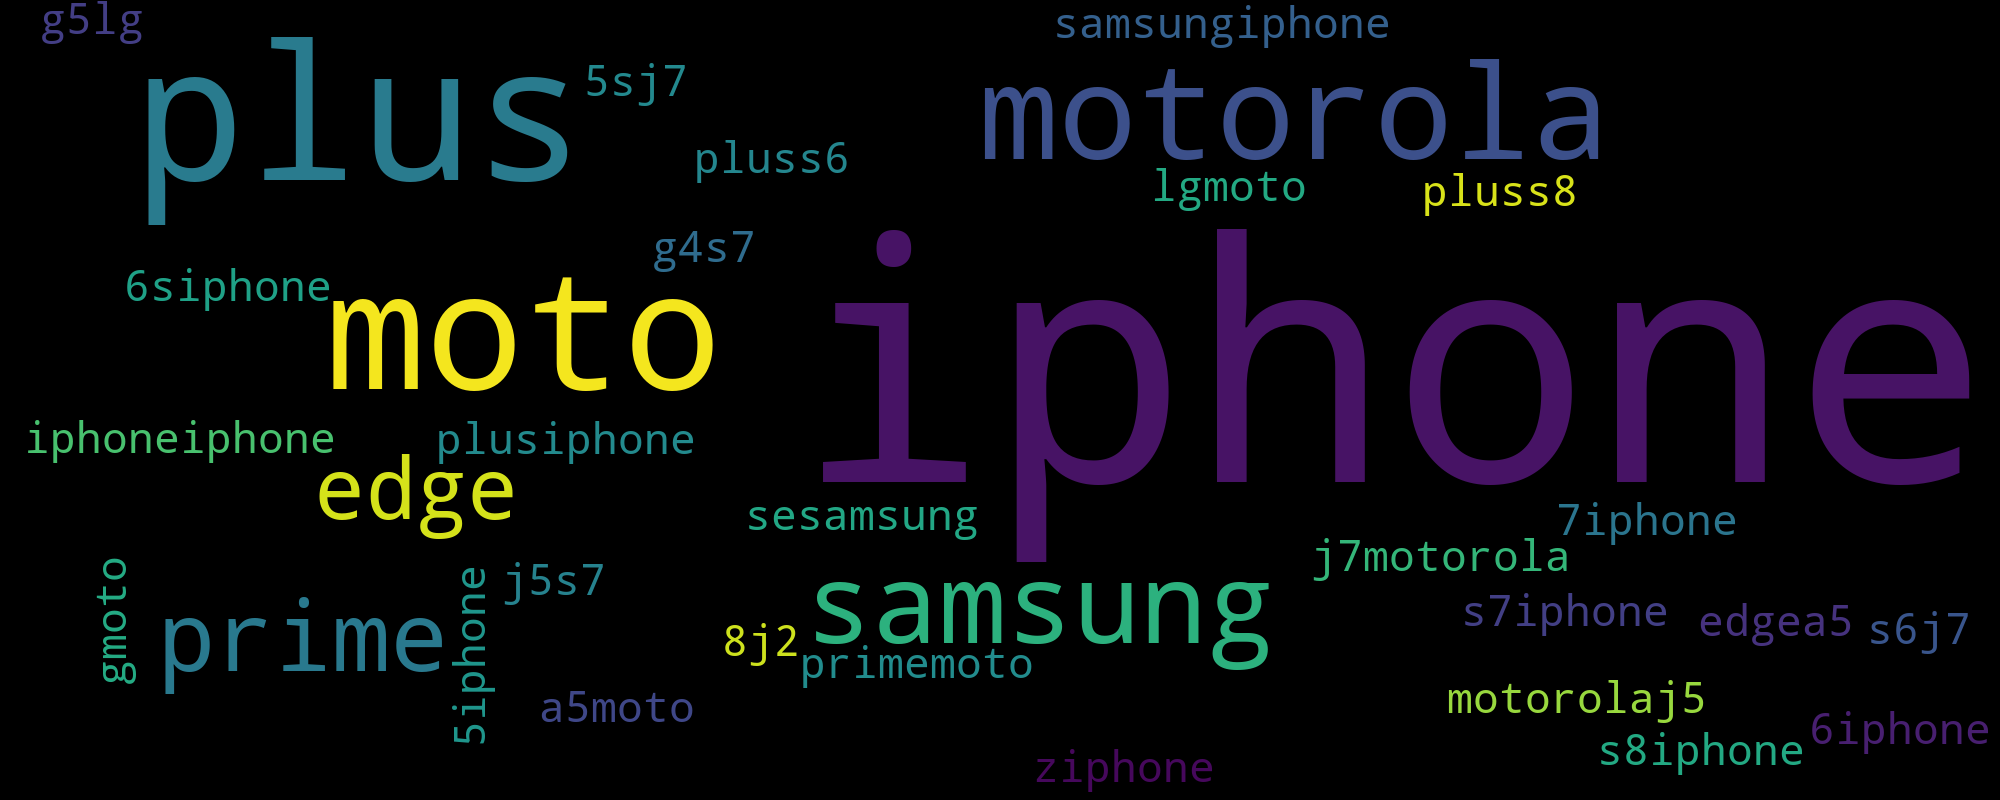
\includegraphics[width=1.2\textwidth]{figures/07-search_terms-wordcloud.png}}
	\caption{Términos más buscados por los usuarios de Trocafone}
	\label{fig:searchedterm}
\end{figure}

Los términos más buscados (vistos en el gráfico \ref{fig:searchedterm}) son \textbf{iPhone}, \textbf{Motorola} y \textbf{Samsung}. Esto era completamente esperable debido a que son las marcas que dominan el sector tecnológico. Se destaca que suelen buscarse más comúnmente la marca de un smartphone antes que un modelo específico.

\subsection{Productos buscados en la plataforma}

En esta sección se busca obtener los productos más buscados. Esta búsqueda es más específica que la anteriormente mencionada debido a que corresponde a un producto puntual, no el nombre de su marca, buscado por la interfaz del sitio. De esta manera los productos más buscados son los que se detallan en la tabla \ref{table:sencilla} y se representan en el gráfico que le sigue.

\begin{table}[!h]
	\begin{center}
		\begin{tabular}{|l|l|}
			\hline
			sku & sku\_name \\
			\hline \hline
			3371 & Samsung Galaxy S6 Flat 32GB Dourado (Bom) \\ \hline			
			2777 & Samsung Galaxy S4 i9505 16GB Preto (Bom) \\ \hline
			6357 & Samsung Galaxy J5 16GB Preto (Bom) \\ \hline
			6413 & Samsung Galaxy J7 16GB Dourado (Bom) \\ \hline
			6371 & Samsung Galaxy J5 16GB Dourado (Bom) \\ \hline
		\end{tabular}
		\caption{SKUs más buscados y su nombre}
		\label{table:sencilla}
	\end{center}
\end{table}

\begin{figure}[!h]
	\makebox[\textwidth][c]{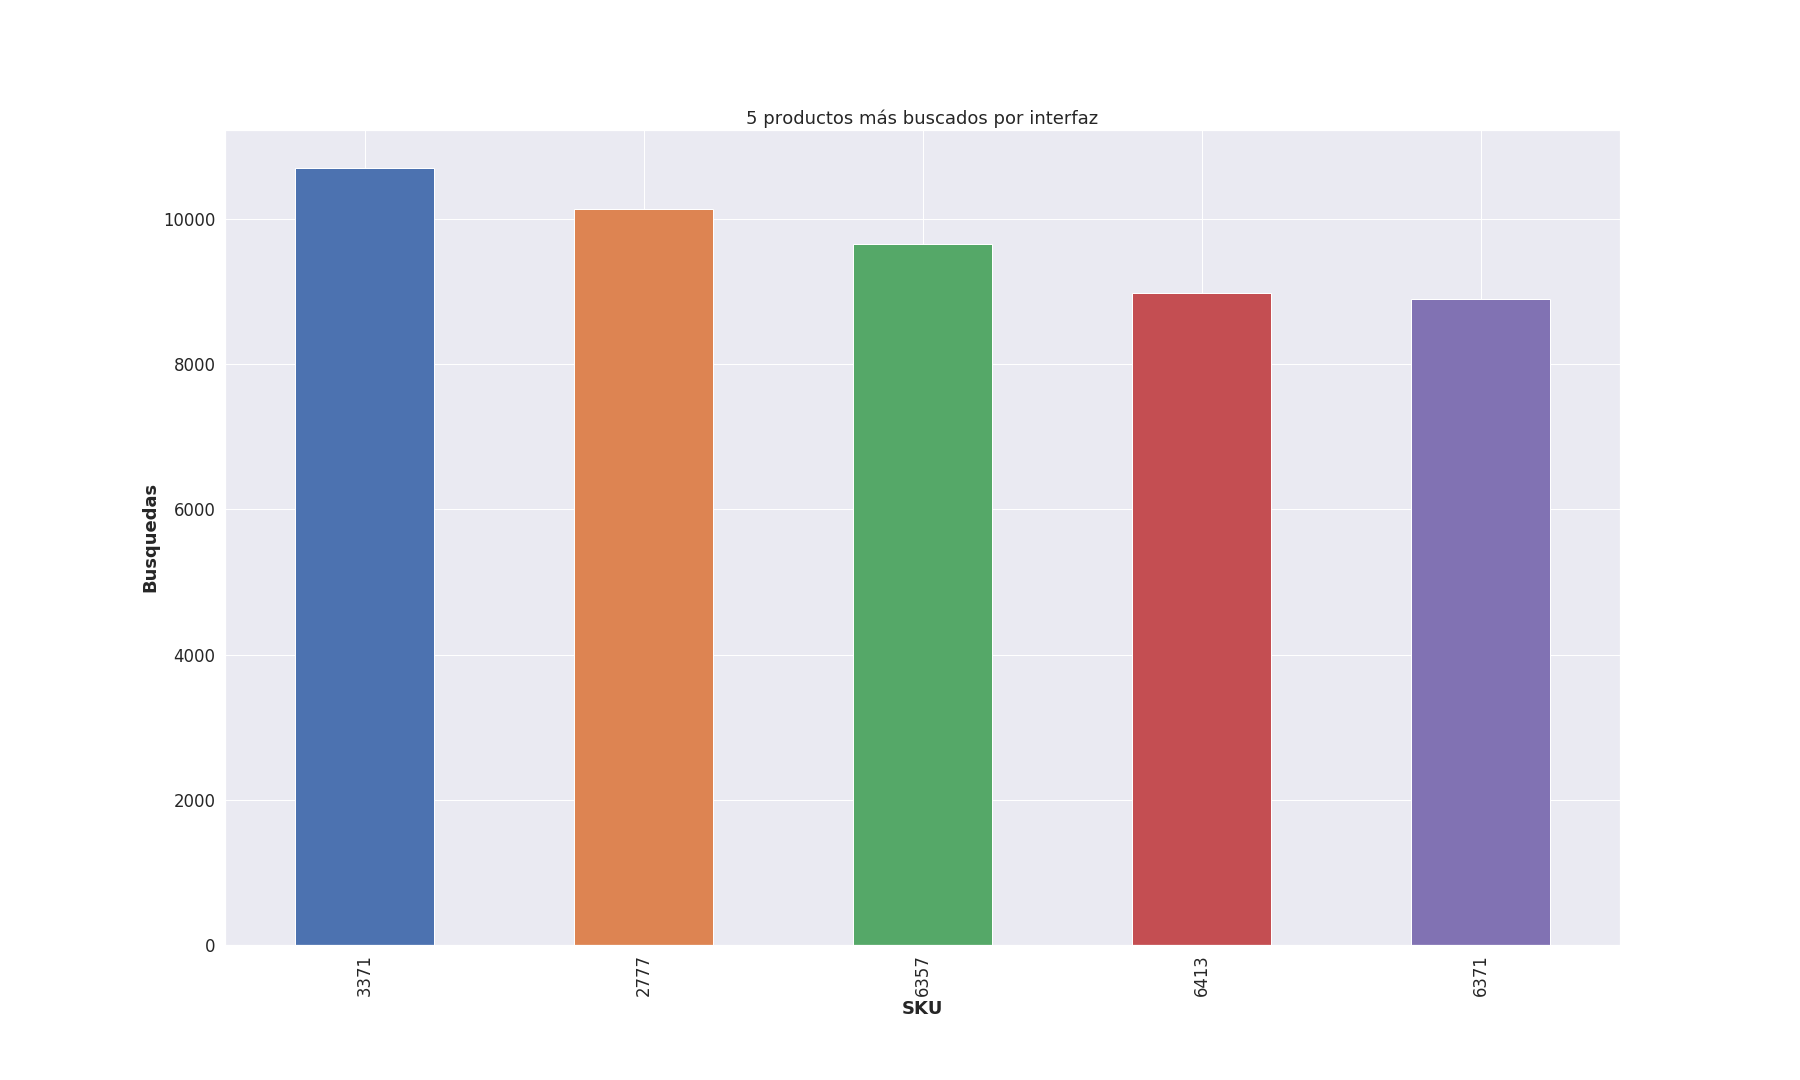
\includegraphics[width=1.2\textwidth]{figures/08-skus_buscados-barplot.png}}
	\caption{Productos más buscados por los usuarios de Trocafone}
	\label{fig:searchedproduct}
\end{figure}

Se concluye con el gráfico \ref{fig:searchedproduct} que si bien \textbf{iPhone} y \textbf{Motorola} eran los \textit{términos} más buscados en la plataforma, no sucede lo mismo con los \textit{productos} buscados ya que todos corresponden a la marca \textbf{Samsung}. Esto puede deberse a un tema de la calidad que ofrece dicha marca o su precio, probablemente más conveniente. Los iPhone se caracterizan por tener un precio difícil de acceder por lo que es probable que sea buscado como término para ver las diferentes opciones globalmente pero que no muchas veces se busque un producto determinado de dicha marca.

\section{Análisis de modelos} \label{modelo}

Pasadas las exploraciones enfocadas sobre el sitio web en sí, como sus busquedas o las nacionalidades de sus usuarios, ahora se pone el foco sobre el contenido del sitio, las compras de celulares, específicamente sobre que modelos son los más vistos, comprados y en general con más tráfico.

\subsection{Relación entre ver, llevar al carrito y comprar un celular}

La primera pregunta a hacerse acerca de los celulares es si hay alguna relación directa entre ver un modelo, decidir comprarlo y efectivamente comprar ese mismo modelo. La pregunta surge de la inquietud de si hay efectividad una vez visto el celular. Por ejemplo, puede darse que alguien vea un celular, lo compare y termine comprando otro, o puede darse que uno entre a visitar la página dedicada a un modelo, vea el precio o la condición y decida mejor optar por otra alternativa.

\begin{table}[!h]
	\begin{center}
		\begin{tabular}{|l|}
			\hline
			modelos prominentes a analizar \\
			\hline \hline
			Samsung Galaxy J5 \\ \hline
			Samsung Galaxy S6 Flat \\ \hline
			Samsung Galaxy S7 \\ \hline
			Samsung Galaxy S7 Edge \\ \hline
			iPhone 5s \\ \hline
			iPhone 6 \\ \hline
			iPhone 6S \\ \hline
			iPhone 7 \\ \hline
		\end{tabular}
		\caption{Subconjunto de modelos prominentes}
		\label{table:modelos_prominentes}
	\end{center}
\end{table}

Entonces, se comienza decidiendo un subconjunto de modelos a analizar, para tener una muestra del sitio. Este set, presentado en la tabla \ref{table:modelos_prominentes}, está generado teniendo en cuenta y uniendo los celulares más vistos (\texttt{viewed product}) con los más "llevados al carrito" (\texttt{checkout}) con los más comprados (\texttt{conversion}). Esto es porque de analizar los eventos y los modelos se ve que los eventos (más relevantes\footnote{se descarta del análisis el evento \texttt{lead} por no ser relevante al caso}) que tienen un modelo asociado son esos tres, y es así como se modela la cronología ordenada ideal de eventos desde el punto de vista de un dispositivo:

\begin{enumerate}
\item \textbf{\texttt{viewed product}: Visitar un producto.}
\item \textbf{\texttt{checkout}: Decidir comprarlo.}
\item \textbf{\texttt{conversion}: Efectivamente comprarlo.}
\end{enumerate}

\begin{figure}[!h]
	\makebox[\textwidth][c]{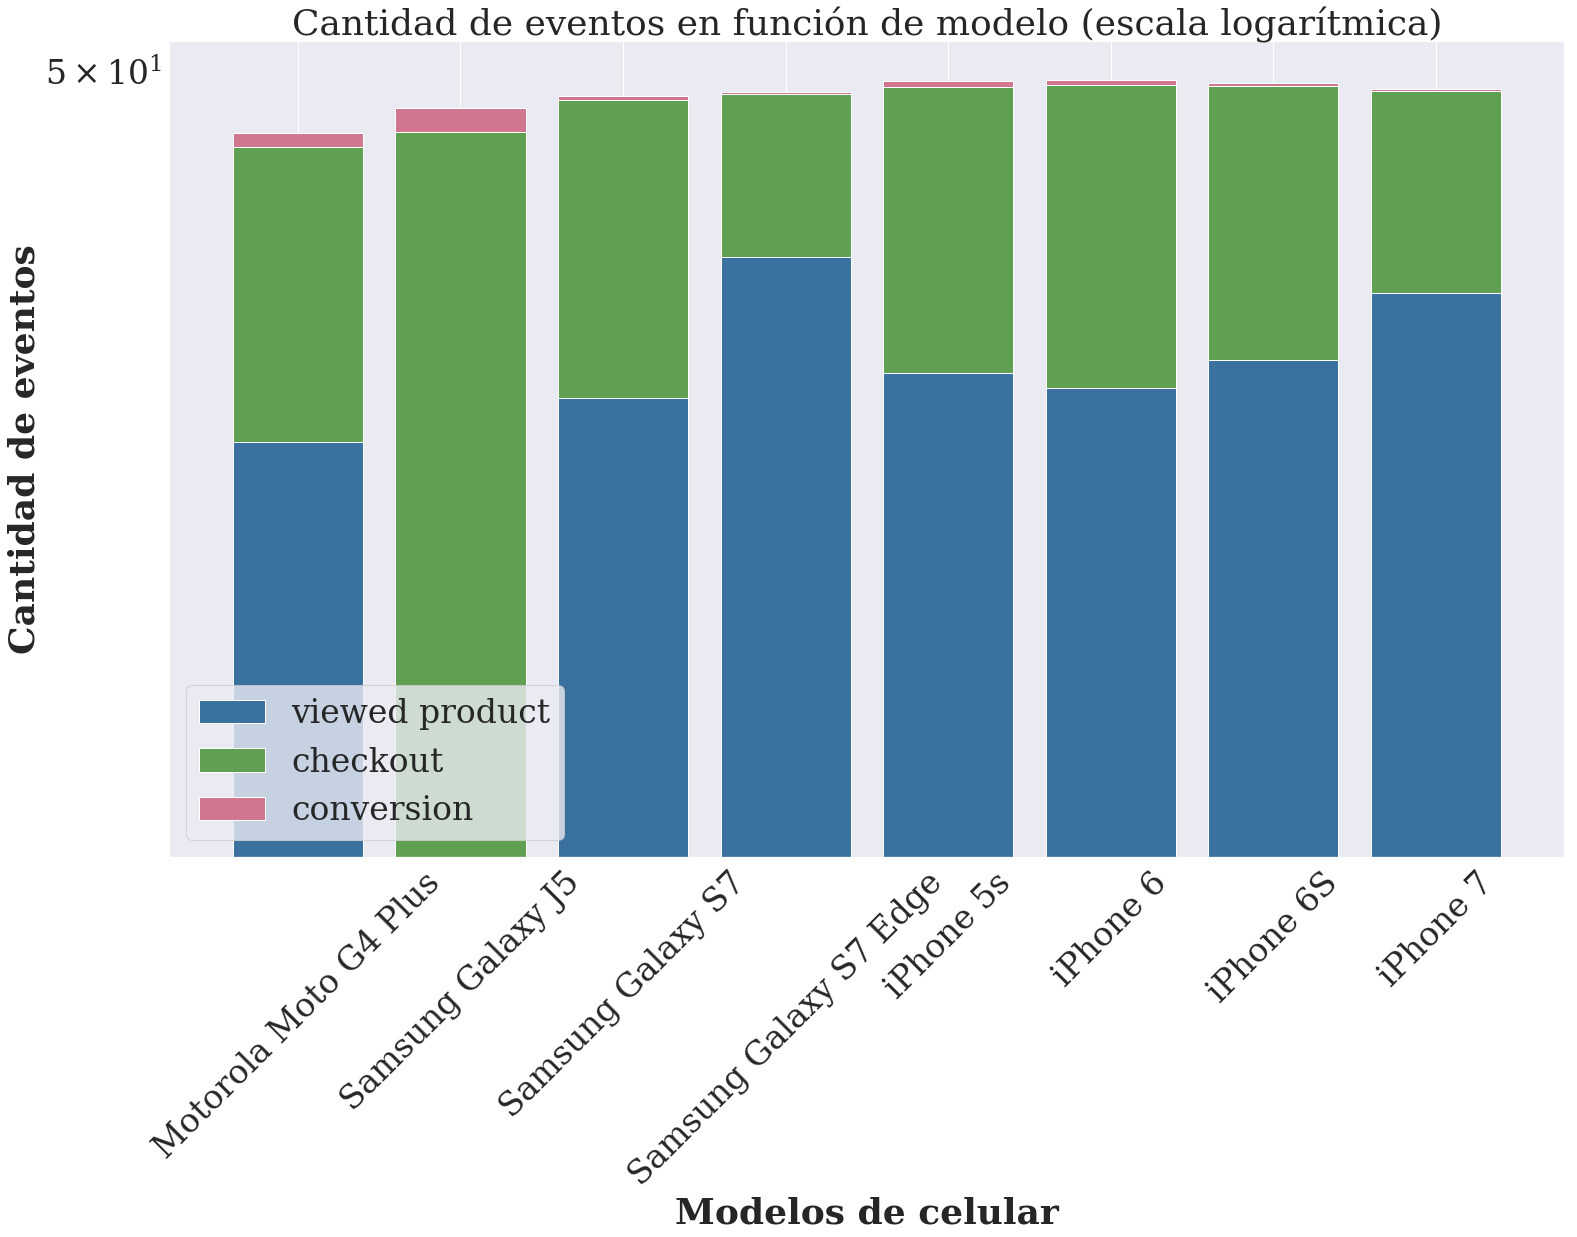
\includegraphics[width=1.2\textwidth]{figures/090-modelos_eventos-stackedbarplot.png}}
	\caption{Cronología de eventos de una muestra de modelos analizados}
	\label{fig:prominentes}
\end{figure}

Primero, en el gráfico \ref{fig:prominentes} se analiza como varían los tres eventos según cada celular. Lo que más se puede notar es que los celulares \textbf{Samsung Galaxy S7 Edge} y \textbf{iPhone 7}, los celulares de mayor gama del sitio son mucho más vistos que el resto, y que verlos es su propio evento predominante por amplia diferencia. Esto se deduce que sucede por el precio y calidad de estos teléfonos; son celulares muy codiciados pero a su vez muy caros, por ende su precio suele ahuyentar compras, pero su calidad atrae visitas.

Lo que no se notó en el primer gráfico fue alguna relación directa entre las marcas de los celulares analizados, en particular si hay algun patrón de \textbf{Apple} vs \textbf{Samsung}.

\begin{figure}[!h]
	\makebox[\textwidth][c]{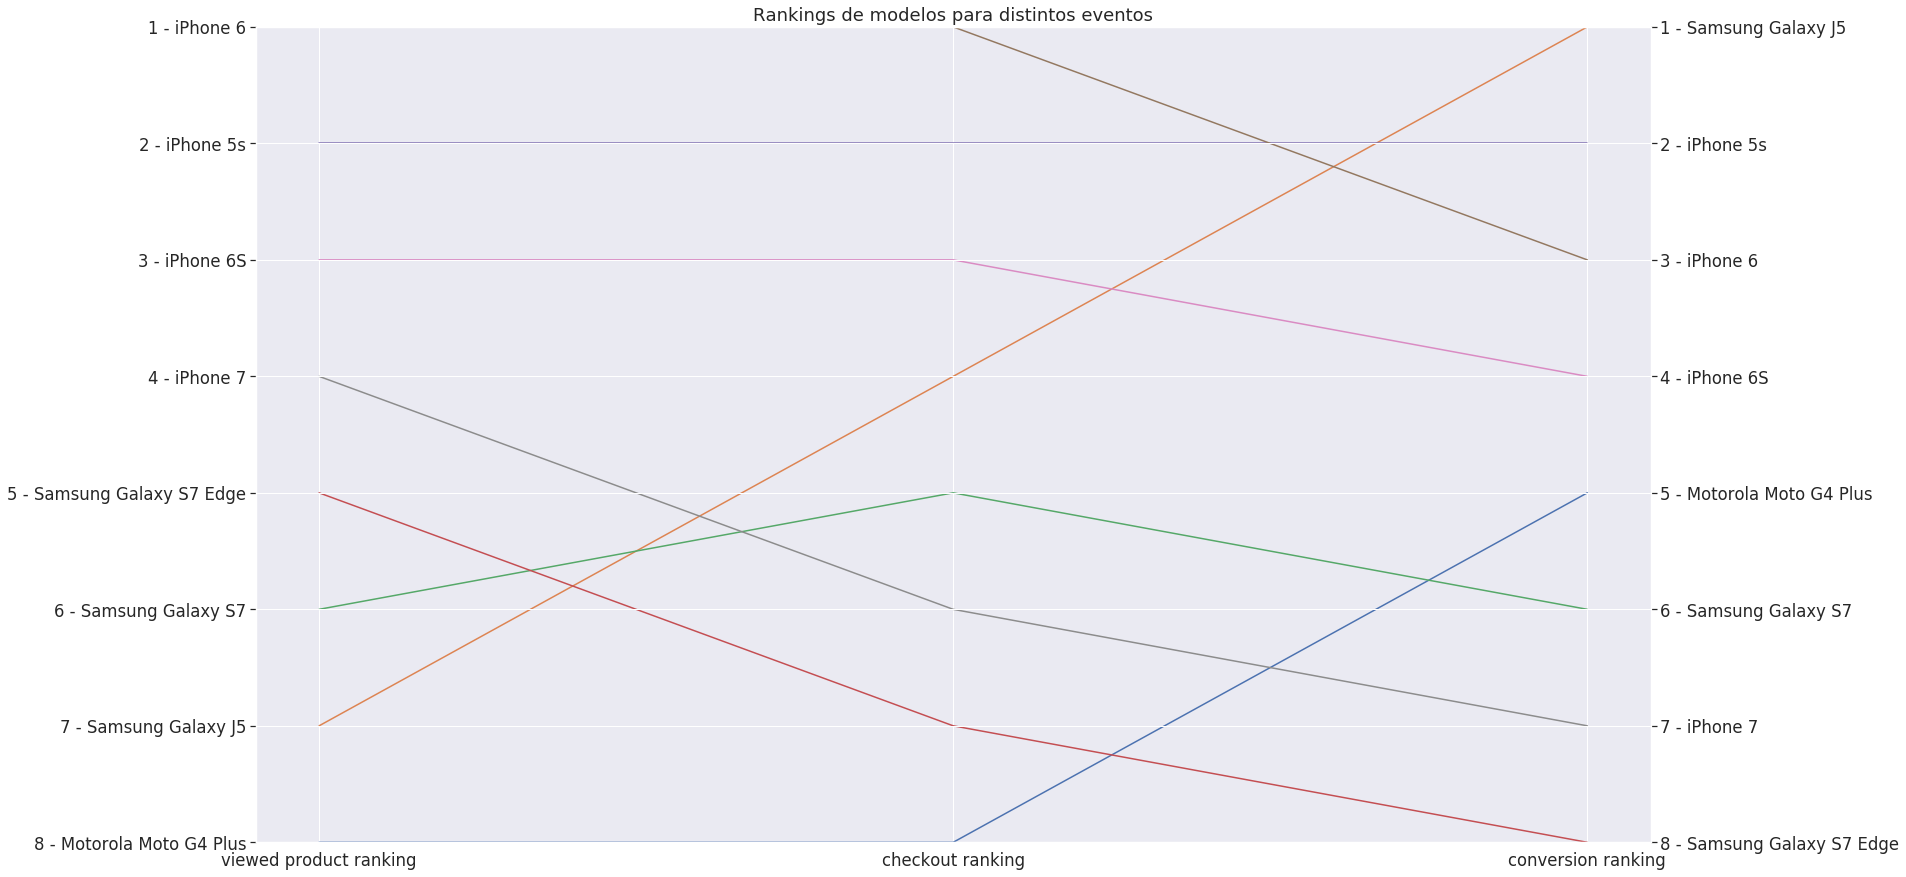
\includegraphics[width=1.2\textwidth]{figures/091-rankings_celulares-rank.png}}
	\caption{Ranking de modelos prominentes según evento}
	\label{fig:prominentesrank}
\end{figure}

En el gráfico \ref{fig:prominentesrank} se puede ver el ranking de cada celular dependiendo de su evento. Mientras más alto el celular, más eventos tiene. Si bien este gráfico esquiva los números exactos, sirve para ver la posición de cada celular respecto de los otros. Lo que se nota acá es similar a lo dicho anteriormente, a mayor calidad de celular, más visitas, pero esto conlleva mayor precio y por ende menos compras. Algunos casos en particular a ver son el \textbf{Samsung Galaxy J5} y el \textbf{Samsung Galaxy S6 Flat} que son de los celulares menos buscados pero a su vez de los más comprados, y como caso inverso presentado, se ve que el \textbf{iPhone 6} y \textbf{iPhone 7} cumplen el rol opuesto, siendo de los celulares más vistos pero menos comprados.

También, hay una pequeña relación a destacar de las marcas de celulares, donde de los 8 modelos analizados, los 4 celulares más buscados son los de marca \textbf{Apple} y los 4 menos buscados son los de su rival, mientras que en la compra pasa (casi) exactamente lo inverso. Se podría presentar un caso de que el análisis de a mayor calidad y precio hay más vistas y menos compras no solo aplica para modelos si no que también para marcas en general, pero esto excede al trabajo presentado.

\subsection{Relación entre celulares y sus condiciones}

Habiendo encontrado un tan rico análisis entre eventos y celulares, se busca con el mismo objetivo una relación entre la condición de uso del celular y su tráfico. Trocafone clasifica los celulares reacondicionados en \textbf{Bueno}, \textbf{Muy Bueno} y \textbf{Excelente} (no se tienen en cuenta los celulares de conidición \textbf{Nuevo} en el presente análisis). Queremos encontrar un patrón de compra y visita de los modelos analizados previamente, pero esta vez según condición.

\begin{figure}[!h]
	\makebox[\textwidth][c]{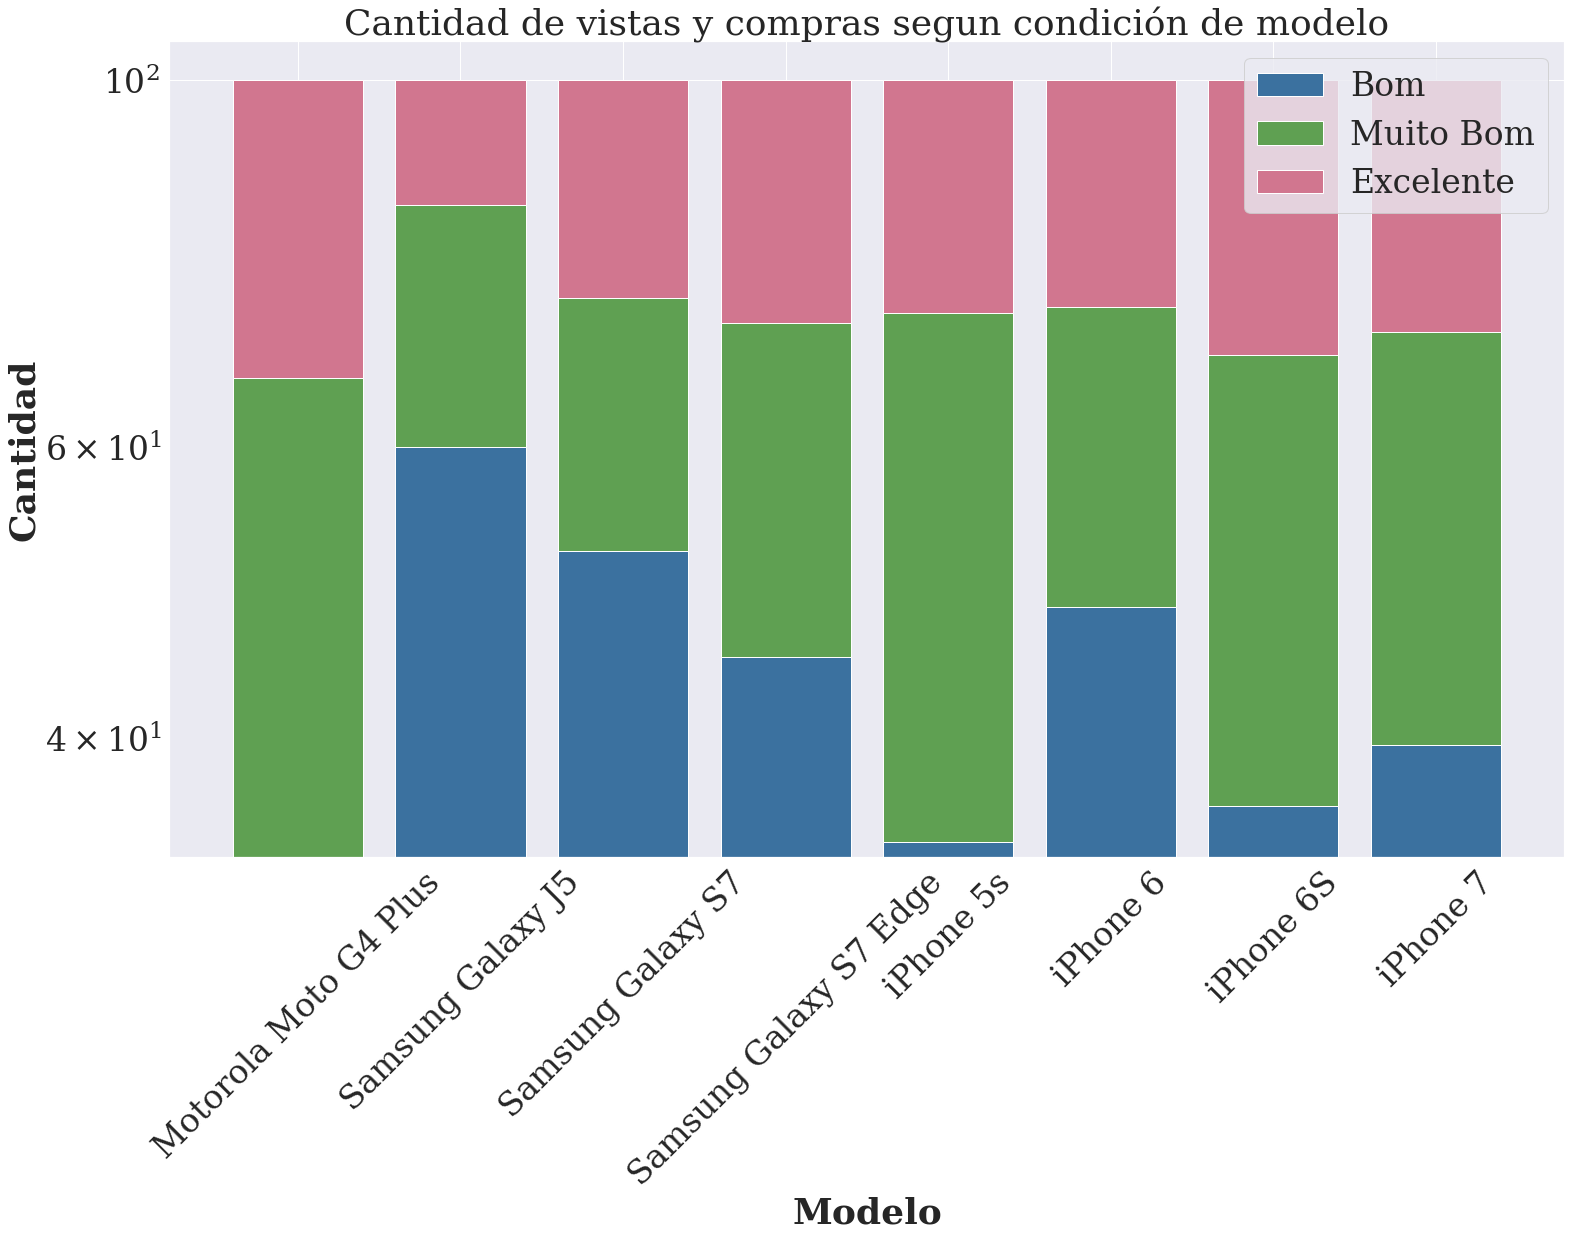
\includegraphics[width=1.2\textwidth]{figures/10-condicion-stackedbarplot.png}}
	\caption{Eventos en modelos según condición}
	\label{fig:prominentescondicion}
\end{figure}

Lo que vemos nuevamente, esta vez en el gráfico \ref{fig:prominentescondicion} es que hay una diferencia substancial entre celulares marca \textbf{Apple} y celulares marca \textbf{Samsung}. Para la marca \textbf{Samsung} se ve como hay mayor tráfico en los modelos de menor condición, sugiriendo el estar dispuesto a comprar celulares no en perfecto estado, mientras que para los \textbf{Apple} aparenta haber una demanda por celulares en muy buena condición, insinuando que se quiere excelencia tanto en calidad de software (responsabilidad de \textbf{Apple}) como en calidad de hardware (responsabilidad de \textbf{Trocafone}).

\subsection{Colores de dispositivos}

\begin{figure}[!h]
	\makebox[\textwidth][c]{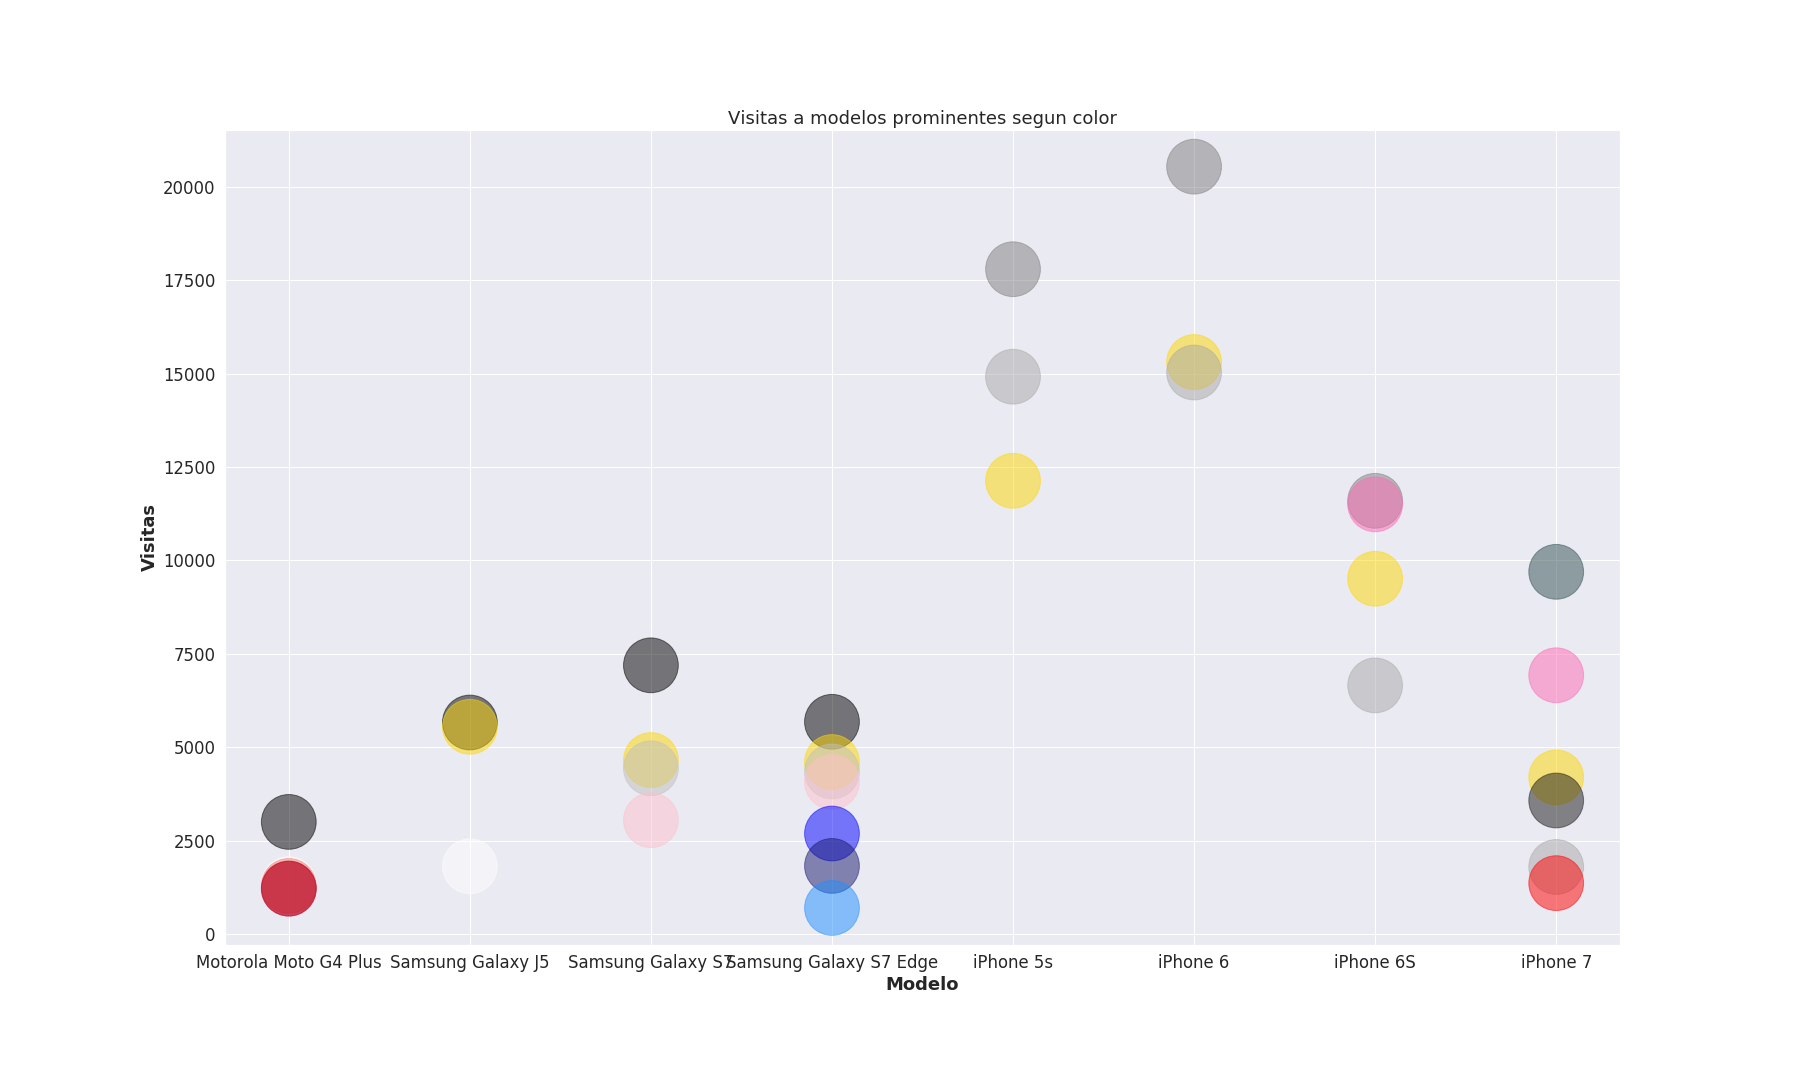
\includegraphics[width=1.2\textwidth]{figures/11-colores-bubbleplot.png}}
	\caption{Colores con más tráfico}
	\label{fig:colores}
\end{figure}

Para concluir la sección se muestran en el gráfico \ref{fig:colores} los colores de los celulares analizados previamente, solo a modo ilustrativo ya que poco se puede extraer y co-relacionar de algo tan arbitrario y subjetivo como la elección de un color de un celular a comprar (aunque si se nota un parcial desbalanceo (\textit{skewness}) hacia los celulares con tintes grises y/o plateados).

\section{Análisis de páginas estáticas}

Se propone comparar la cantidad de visitas al \texttt{FAQ}\footnote{Frequently Asked Questions: lista de preguntas y respuestas que surgen comúnmente en un contexto determinado.} con las de \texttt{Customer Service}, para poder analizar la forma que tiene \textbf{Trocafone} de brindar soporte a sus usuarios.

\begin{figure}[!h]
	\makebox[\textwidth][c]{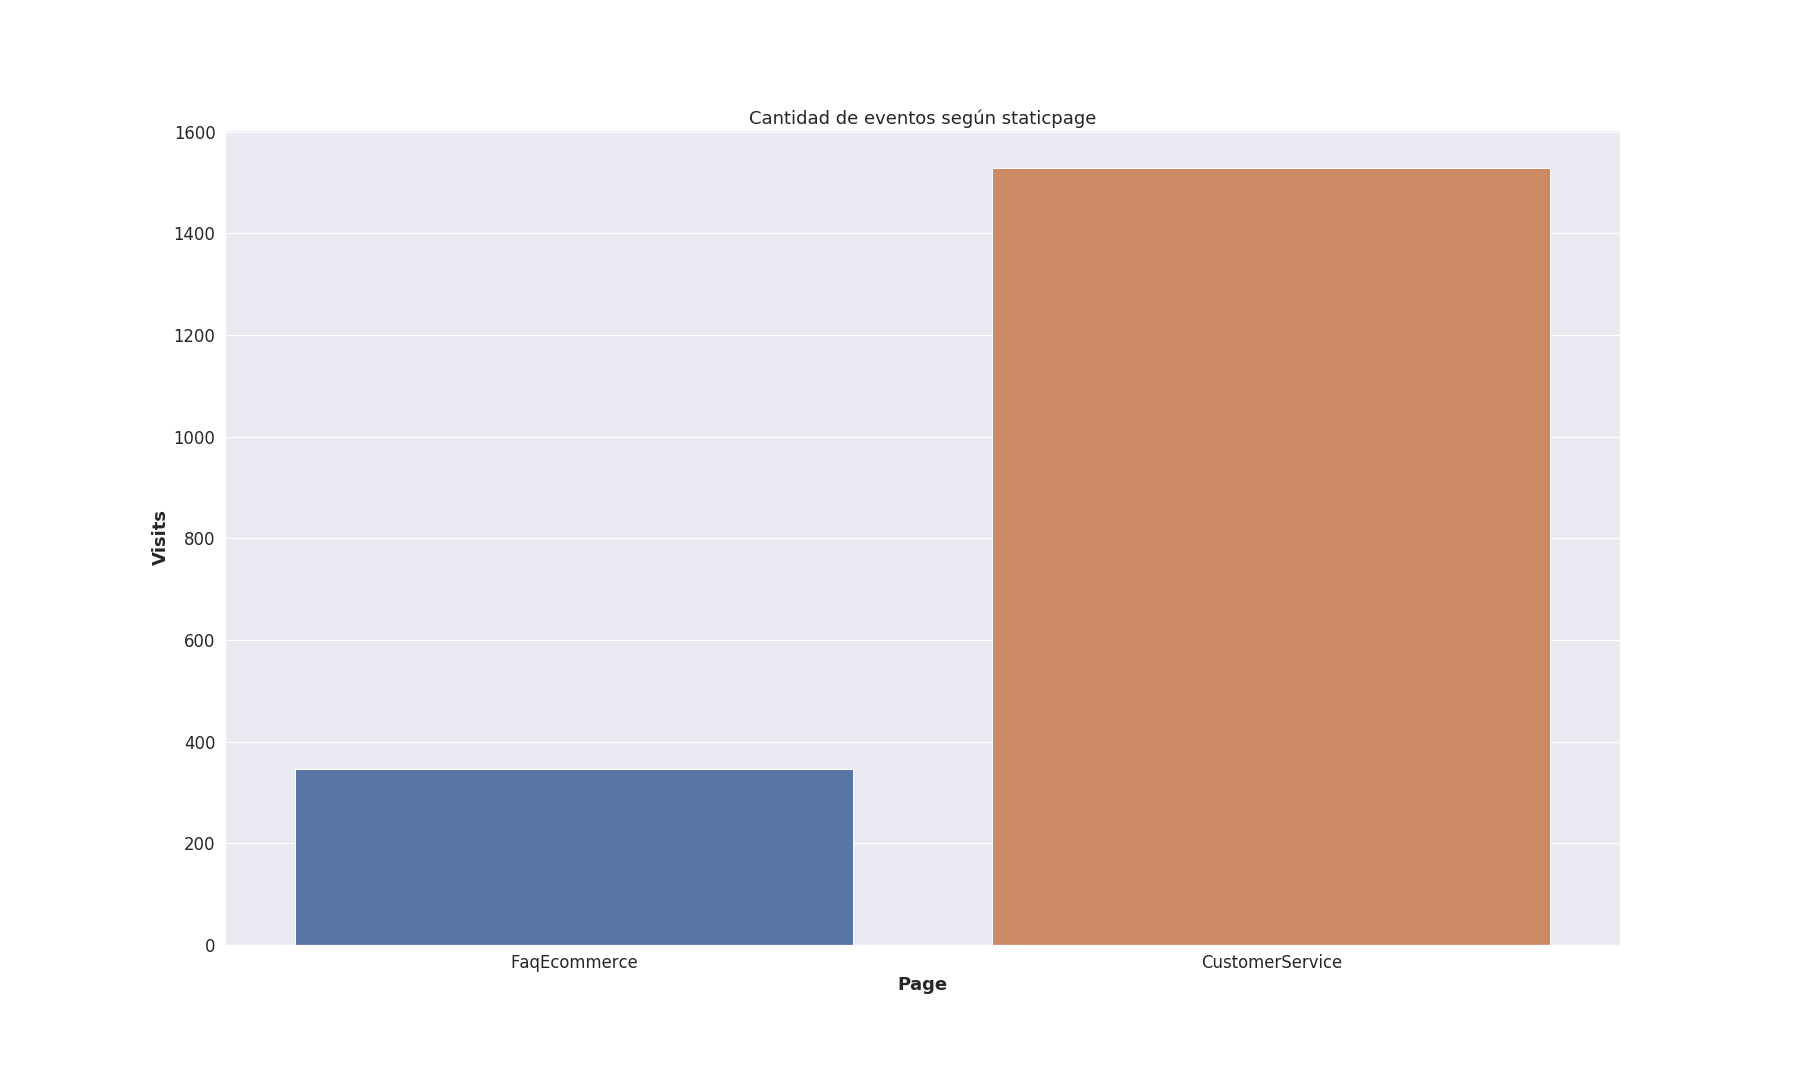
\includegraphics[width=1.2\textwidth]{figures/12-static_pages-barplot.png}}
	\caption{Comparación entre cantidad de visitas al FAQ y a Customer Service}
	\label{fig:staticpage}
\end{figure}

Del gráfico \ref{fig:staticpage} se ve que la cantidad de visitas a \texttt{Customer Service} es mucho mayor que la cantidad de visitas al \texttt{FAQ}. Para mantener la página de \texttt{Customer Service} es necesario disponer de empleados constantemente para responder las consultas requeridas. Por lo tanto, se podría optimizar recursos redireccionando parte del tráfico a FAQ, haciendo más visibles los links a la página, agregando contenido común y mejorándola de ser necesario.

\section{Análisis de nuevos usuarios vs usuarios que regresan al sitio}

En esta sección se busca determinar la proporción de usuarios del sitio que entraron una sola vez a la página y no volvieron a hacerlo. Para ello se grafica en un primer lugar la cantidad de usuarios calificados como \texttt{New} contra los que son calificados como \texttt{Returning}.

\begin{figure}[!h]
	\makebox[\textwidth][c]{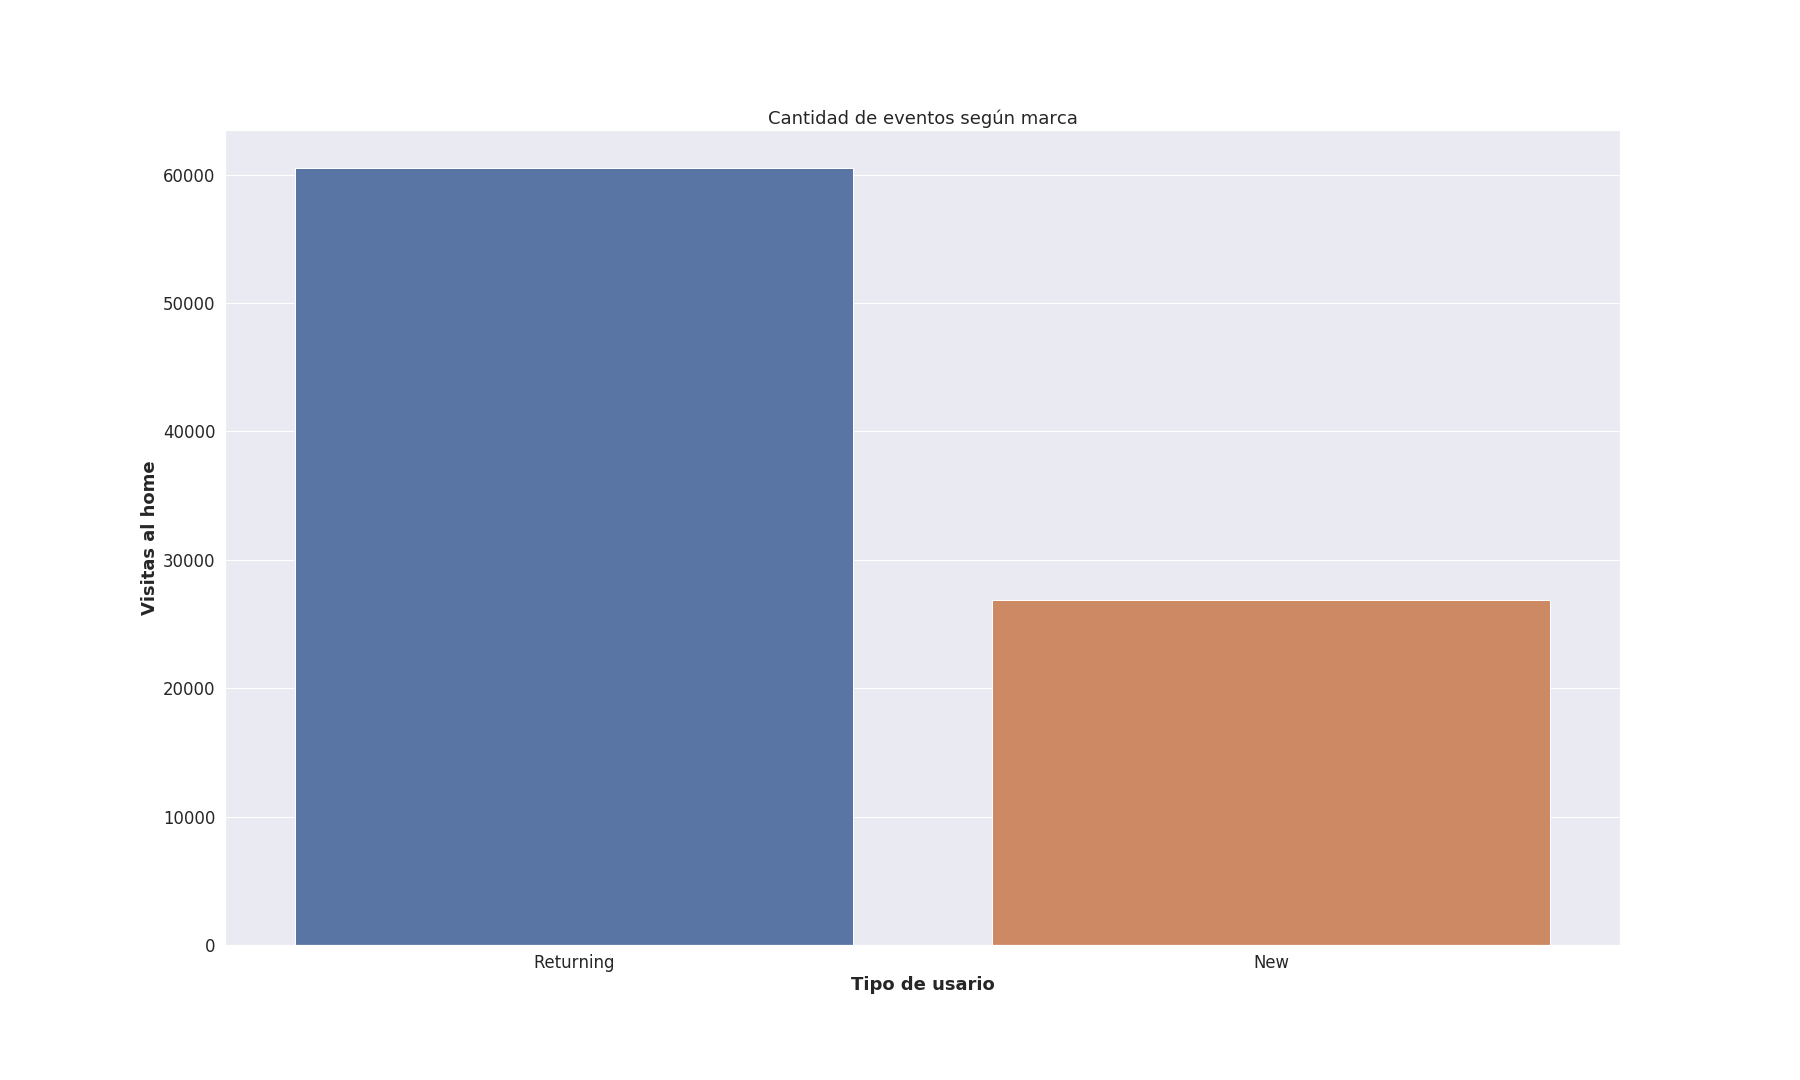
\includegraphics[width=1.2\textwidth]{figures/130-eventos_new_returning-barplot.png}}
	\caption{Comparación entre cantidad de usuarios que entran por primera vez al sitio contra los que volvieron}
	\label{fig:newvsreturningfalse}
\end{figure}

Es necesario remarcar que el gráfico \ref{fig:newvsreturningfalse} no es representativo porque todos los usuarios calificados como \texttt{returning} en algún momento fueron registrados como \texttt{new} (su primera vez ingresando al sitio). A simple vista se podría concluir que la proporción de usuarios que regresa es mucho mayor a los que entran solo una vez. 

Se realiza el recorte necesario para obtener una visualización que refleje fiablemente la cantidad de visitantes que entra al sitio una sola vez contra los que vuelven otras veces. 

\begin{figure}[!h]
	\makebox[\textwidth][c]{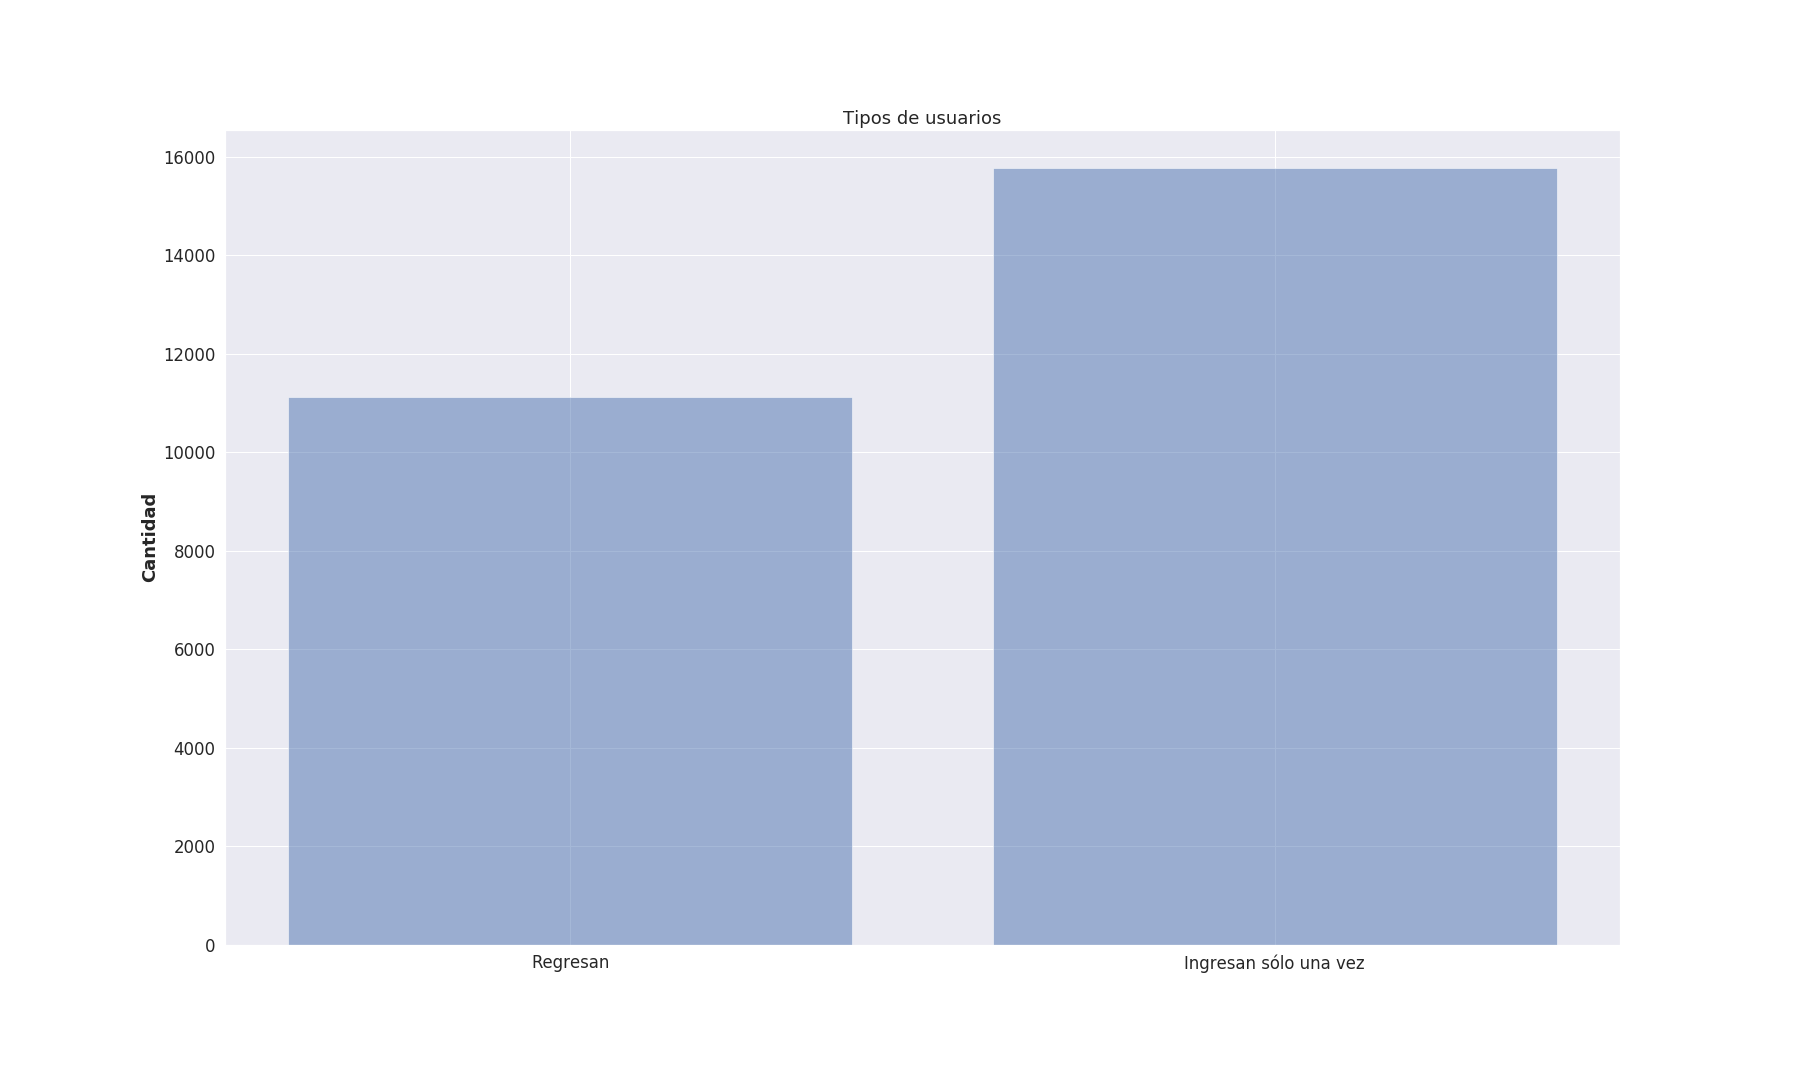
\includegraphics[width=1.2\textwidth]{figures/131-tipos_usuarios-barplot.png}}
	\caption{Comparación entre cantidad de usuarios que entran por primera vez al sitio contra los que volvieron}
	\label{fig:newvsreturning}
\end{figure}

Se observa en el gráfico \ref{fig:newvsreturning} que la tasa de personas que entra una sola vez es mayor a la de las que regresan. Esta información desfavorece a Trocafone ya que implica que pierde una gran cantidad de clientes\footnote{Nuevamente se recuerda que estamos hablando del subconjunto de usuarios que realiza al menos un \texttt{checkout}, un subconjunto que se asume mucho menor que el global de los usuarios del sitio.}. Para aumentar la tasa de personas que regresan a ĺa página se puede proponer aumentar el presupuesto en publicidad y mejorar la experiencia de usuario de la home para que provea al usuario una experiencia más amena. También podrían ampliarse los métodos de pago o mejorar la página de \texttt{Customer Service} para que el cliente se sienta más contenido y pueda resolver todos los conflictos existentes ante una compra.

\section{Análisis de marcas}

Se busca determinar qué marcas son las que reúnen la mayor cantidad de eventos. Esto puede ser ya sea porque son las marcas más compradas, más buscadas o más vistas, entre otros eventos. Este análisis es más bien global ya que no es específico a un evento determinado.

\begin{figure}[!h]
	\makebox[\textwidth][c]{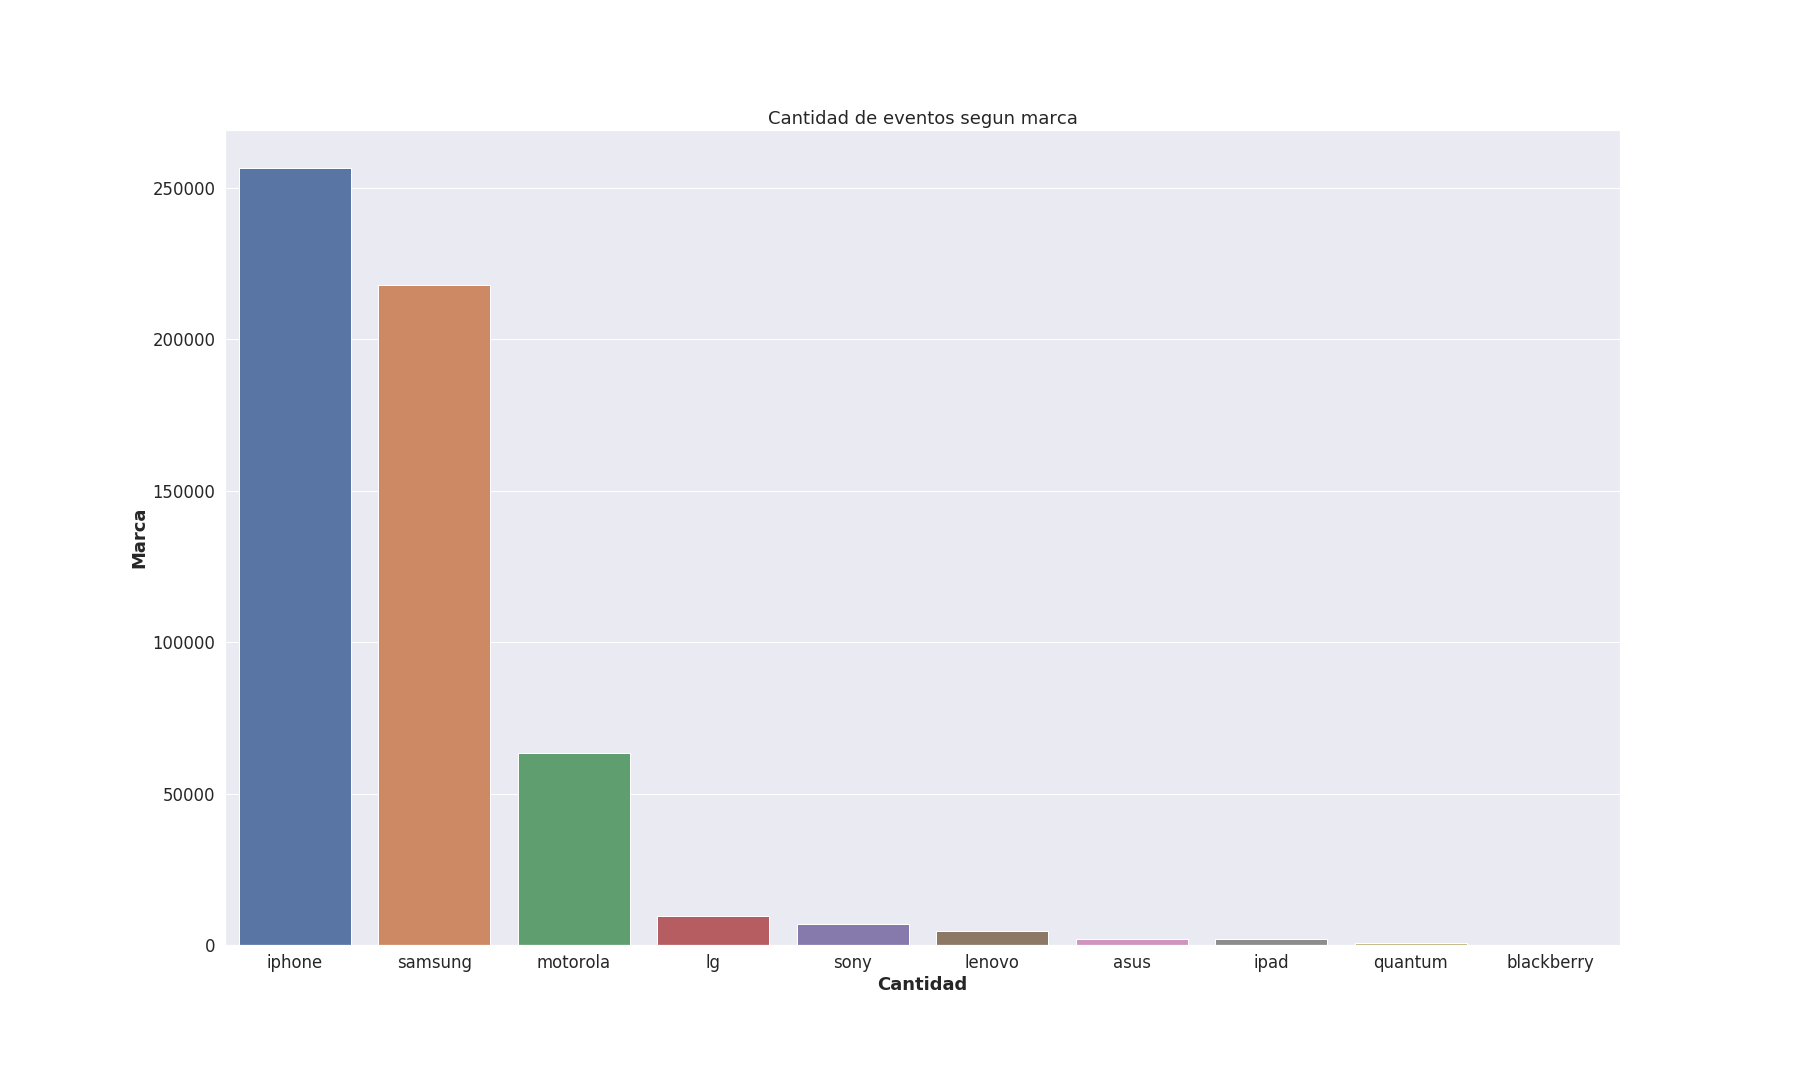
\includegraphics[width=1.2\textwidth]{figures/141-eventos_marca-barplot.png}}
	\caption{Cantidad de eventos según marca}
	\label{fig:freqbrands}
\end{figure}

Se conserva el comportamiento presentado en la sección \ref{busq} con respecto a los términos más buscados. Las marcas que registran mayor cantidad de eventos son \textbf{iPhone}, \textbf{Motorola} y \textbf{Samsung}.

Ahora se busca analizar cuáles marcas son las que realizan una cantidad pareja de checkouts y conversiones. Siguiendo la linea de razonamiento en la sección \ref{modelo} se predice que las marcas que venden celulares a precios elevados como \textbf{Apple} van a mostrar una cantidad mayor de checkouts que conversiones. Así mismo, las marcas que mantienen un precio más accesible van a tener ambas cantidades más parejas. 

\begin{figure}[!h]
	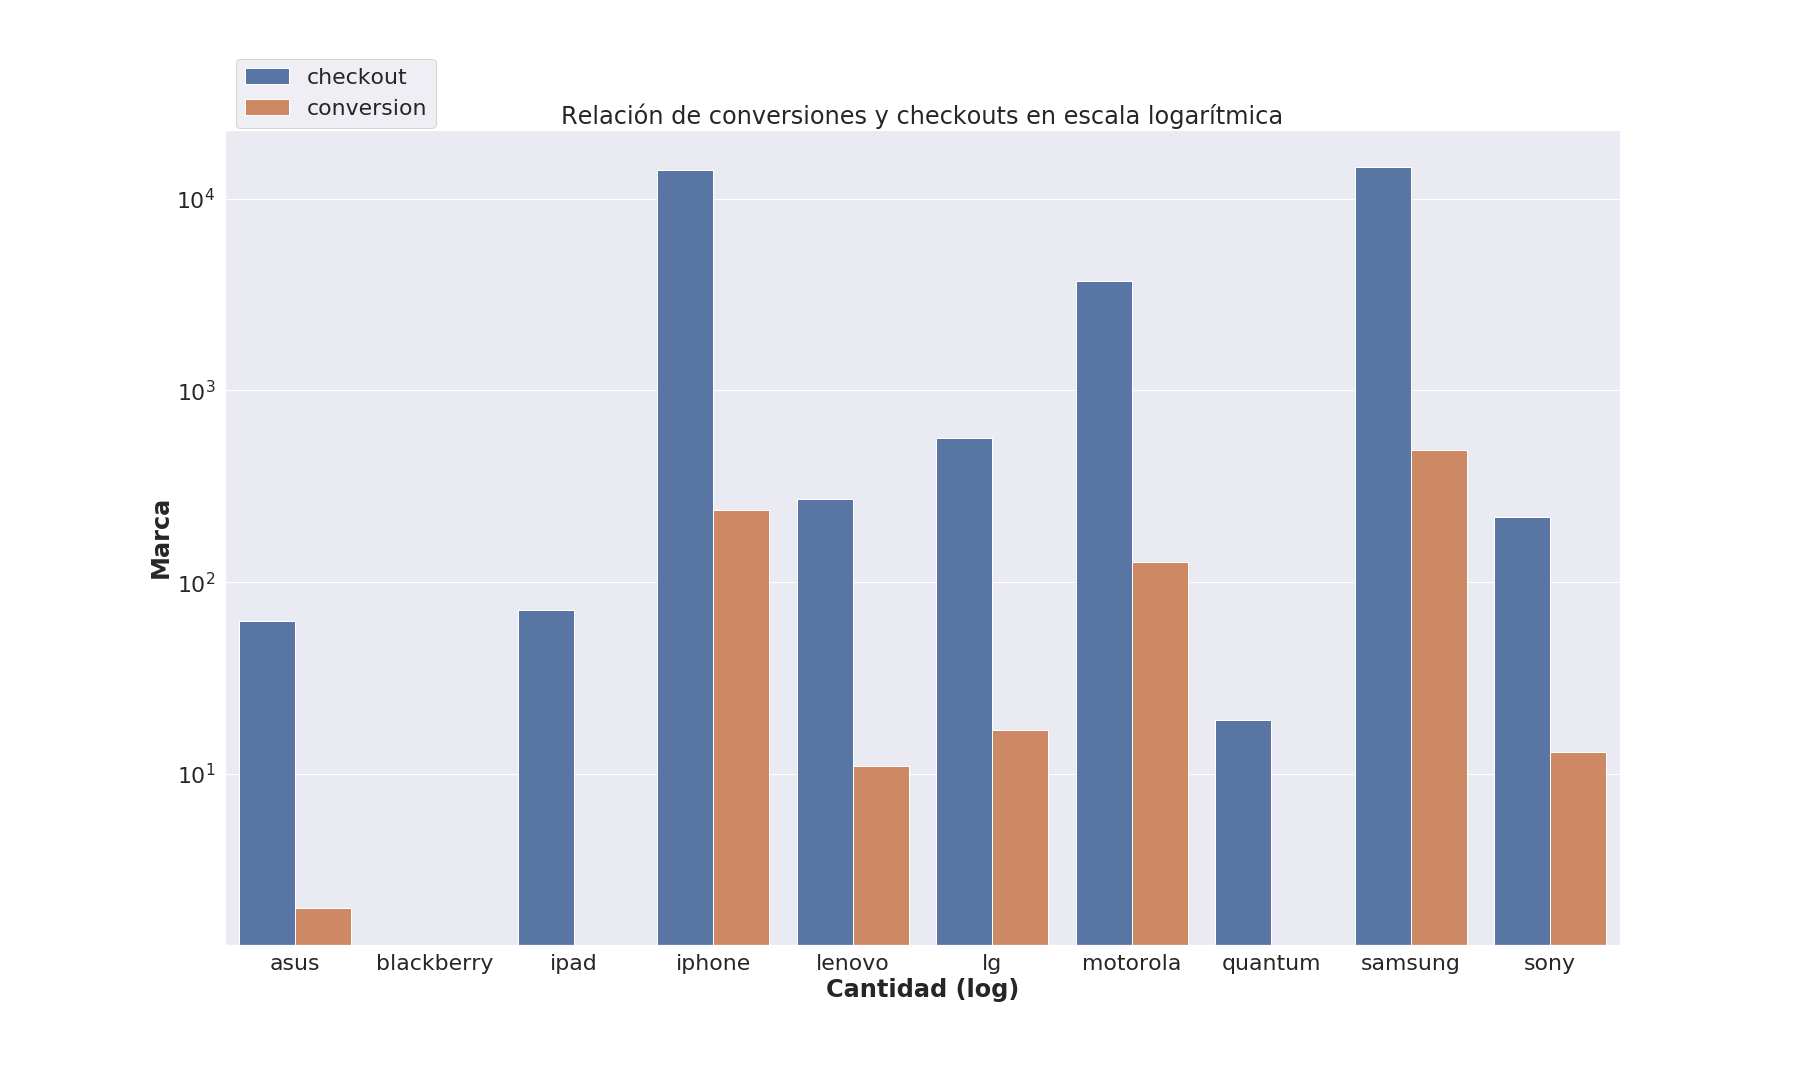
\includegraphics[width=\linewidth]{figures/142-conversiones_checkouts_marca-barplot.png}
	\caption{Checkouts vs conversiones según marca en éscala logarítmica}
	\label{fig:brands}
\end{figure}

Se observa en el gráfico \ref{fig:brands} que la relación checkout-conversions para las marcas representadas es relativamente constante para todas las marcas, con algunas excepciones marcadas donde la cantidad de conversiones es muy chica, como \textbf{Asus}, \textbf{iPad} (técnicamente \textbf{Apple}) o \textbf{Quantum}. Igualmente podría afirmarse que la predicción es cierta porque esta relación es mayor en la marca \textbf{Samsung} que en la marca \textbf{Apple}.

\section{Análisis de tipos de dispositivos}

Se busca analizar en esta sección desde qué tipo de dispositivos suelen acceder los clientes a la página de Trocafone.

\begin{figure}[!h]
	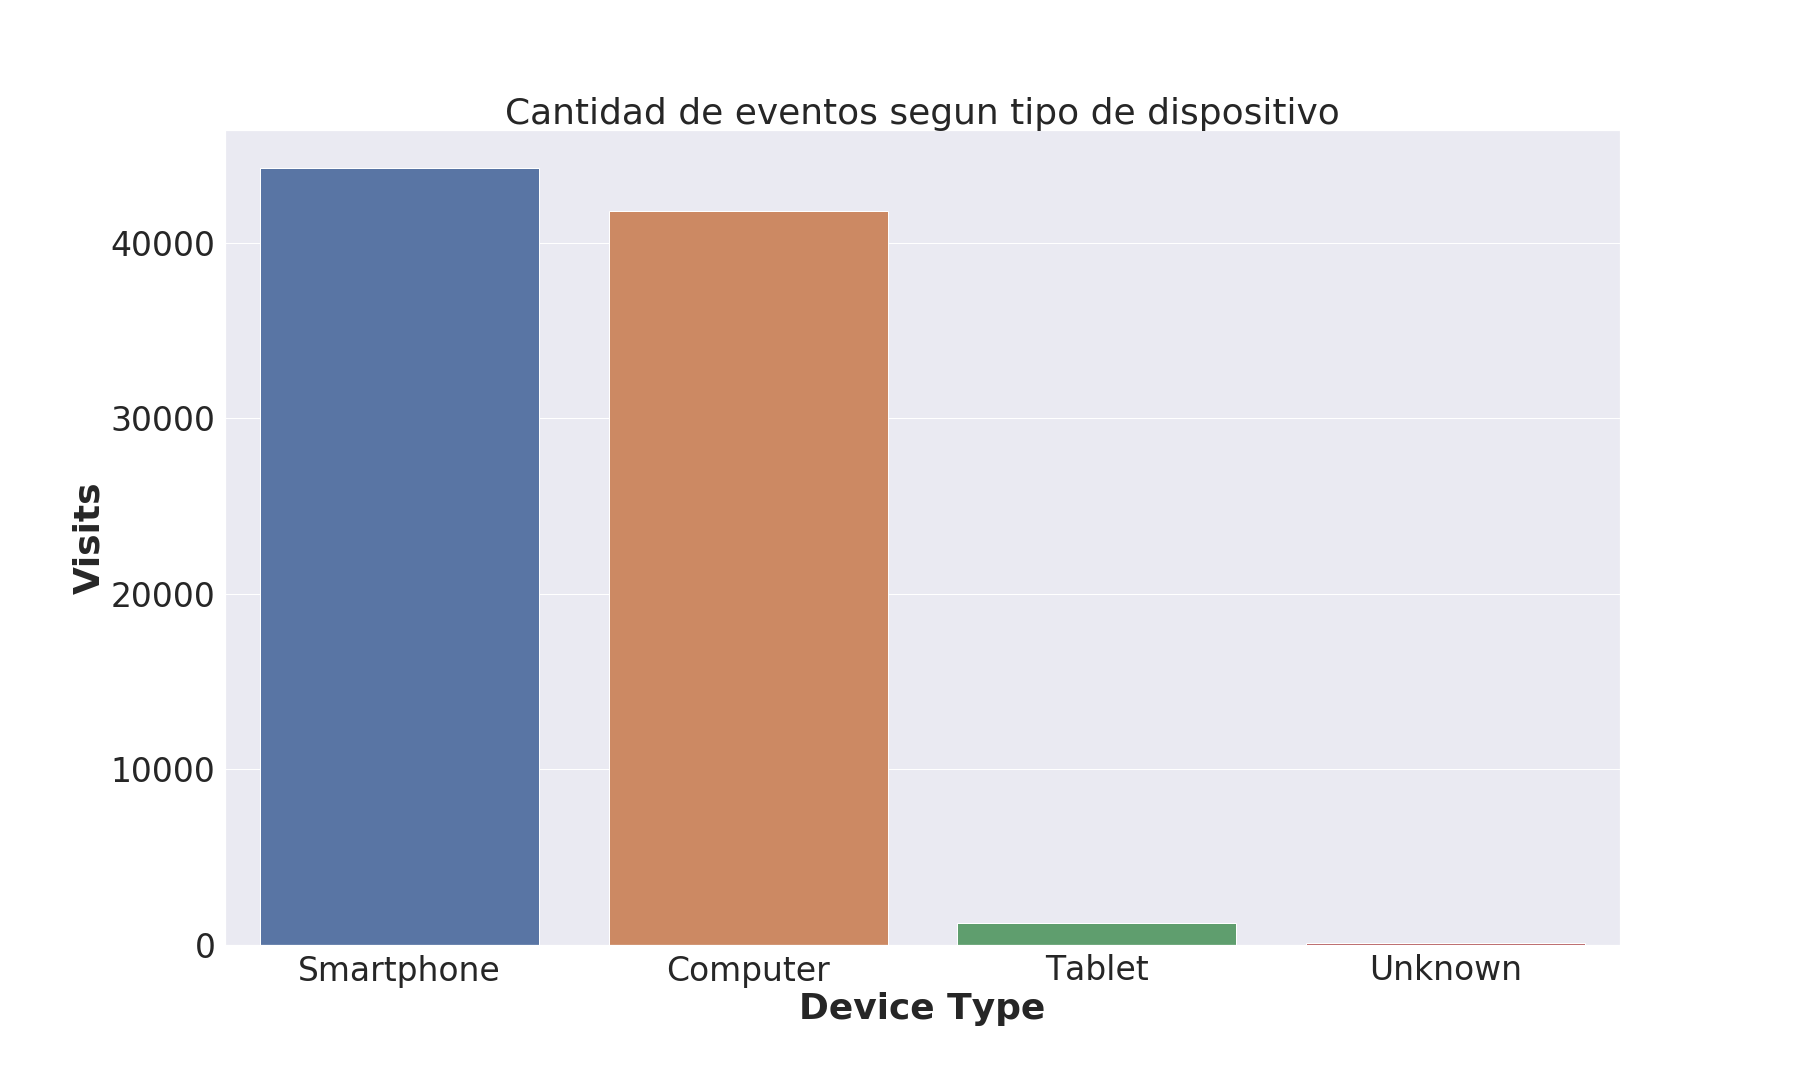
\includegraphics[width=\linewidth]{figures/150-eventos_tipo-barplot.png}
	\caption{Cantidad de eventos de acuerdo al dispositivo utilizado}
	\label{fig:dispositivos}
\end{figure}

Se puede observar en el gráfico \ref{fig:dispositivos} que casi todos los eventos se registran desde un smartphone o una computadora. La cantidad de eventos registrada desde la tablet es significativamente menor. Por lo tanto, se considera que podría dedicarse una mayor cantidad de recursos a desarrollar la aplicación para smartphones y computadoras y no dedicar mucho tiempo y desarrolladores a las aplicaciones para tablets, o bien optar por el camino contrario e intentar hacer más atractiva la manera de ingresar desde la tablet con el fin de atraer nuevos usuarios de ese target en particular, aunque esto implique un mucho mayor costo (se asume que es más dificil y costoso desarrollar algo no exitoso desde el suelo que mantener y mejorar algo con una cantidad constante de visitas).

Lo siguiente a analizar es la fidelidad de los usuarios a sus dispositivos actuales y respectivas marcas y su adversidad al cambio. Implicitamente, lo que también se analiza acá es la efectividad del \textit{branding} de las marcas, ya que mantener consumidores es uno de sus principales objetivos como empresa y se logra con buenas campañas de marketing.

Para poner un ejemplo de fidelidad, un usuario fiel sería quien entra desde una computadora \textbf{Mac} y solo busca para comprarse el \textbf{iPhone} vigente, mientras que un usuario que entra desde \textbf{Android} y decide comprar un \textbf{iPhone} es uno que no es fiel a su marca/sistema operativo actual.

\begin{figure}[!h]
	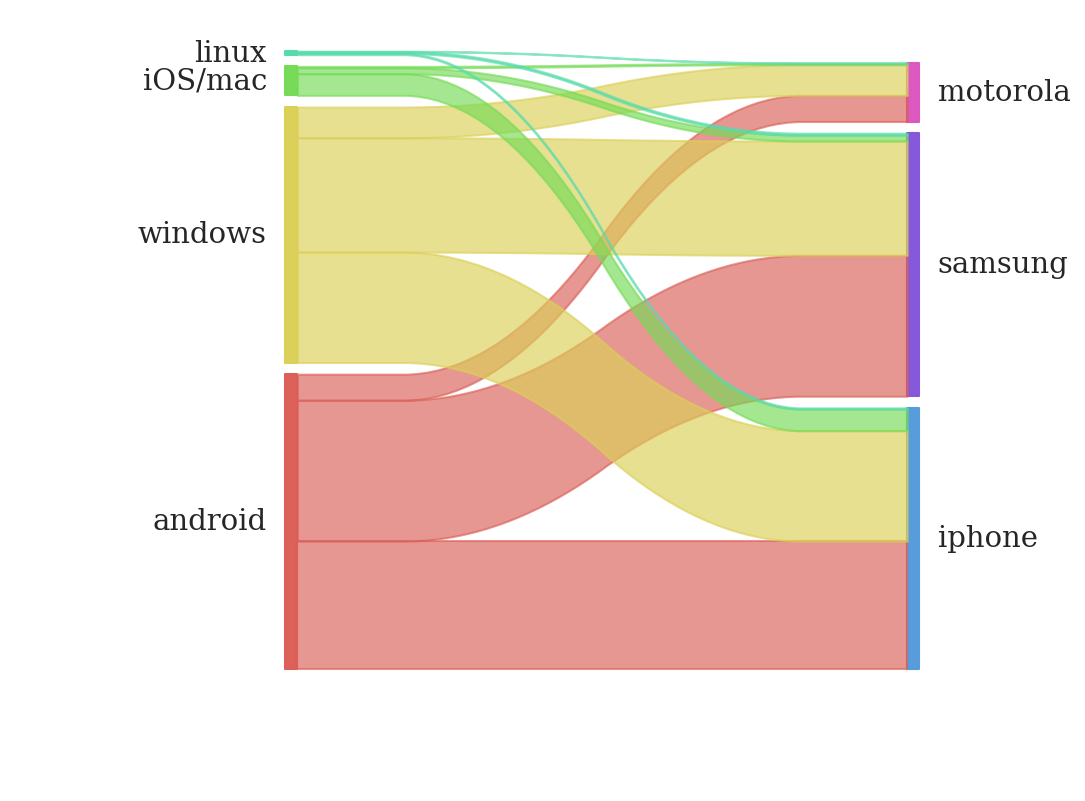
\includegraphics[width=\linewidth]{figures/151-os_brands-sankey.png}
	\caption{Diagrama de flujo de fidelidad de usuarios}
	\label{fig:sankey}
\end{figure}

Notamos en el gráfico \ref{fig:sankey} varias cosas. Por empezar, dada la naturaleza de \textit{branding} y marketing de la empresa, los usuarios de \textbf{Apple} no son muy propensos al cambio y se mantienen en su mayoría sobre su mismo sistema. Por otro lado, los usuarios de \textbf{Android} están uniformemente divididos y no se puede concluir que no sean fieles ni infieles. 

Luego, el caso de \textbf{Windows} sería trivial de analizar, siendo este un sistema operativo de computadoras sin ninguna asociación en particular a marcas de celulares (ignorando el cuasi extinto \textbf{Windows Phone}, que aparecería como la marca \textbf{Nokia} o \textbf{Microsoft}). Y como último es interesante ver los usuarios de \textbf{Linux}, que por la esencia abierta del sistema operativo y su comunidad, es peculiar ver la distribución uniforme (si bien sobre pocos datos) tanto hacia celulares \textbf{Android} como \textbf{Apple}, aún más teniendo en cuenta la fuerte tendencia de este último a ser un sistema más cerrado.

\section{Análisis de publicidad}

La primera pregunta que fue planteada fue la de investigar si \textbf{Trocafone} aumentó el presupuesto en publicidad en algún período de tiempo. Para ello se procede a analizar en qué meses aumentó la cantidad de visitas originadas de una campaña de marketing, información proveída por la columna \texttt{campaign source}.

\begin{figure}[!h]
	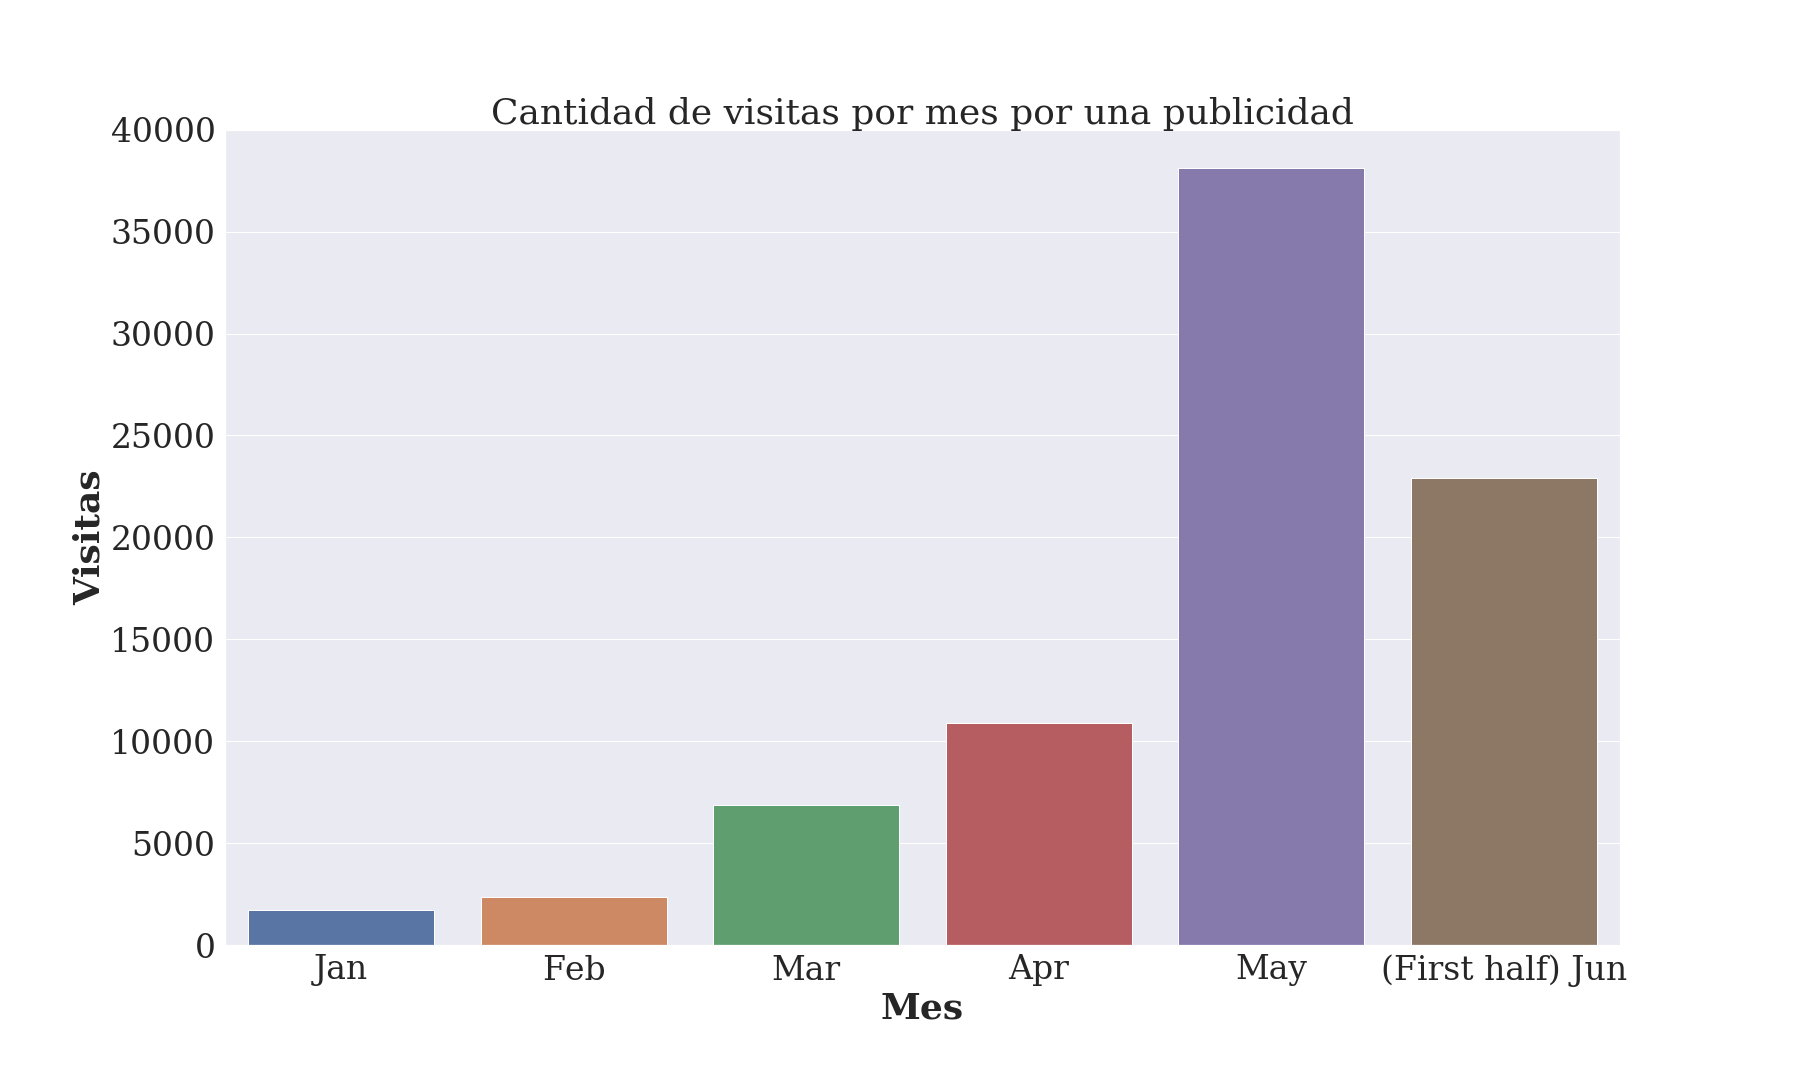
\includegraphics[width=\linewidth]{figures/16-presupuesto-barplot.png}
	\caption{Cantidad de visitas provenientes de una campaña de publicidad de acuerdo al mes}
	\label{fig:publicidad}
\end{figure}

\newpage

La observación del gráfico \ref{fig:publicidad} no permite extraer ninguna conclusión válida. Esto se debe a que el mes en el que se registra mayor cantidad de visitas provenientes de una campaña de publicidad (mayo) es el mes en el que se detectó mayor cantidad de eventos. Sería pensamiento circular decir que hay más visitas este mes porque aumento el presupuesto publicitario si nuestro único fundamento sobre esto esta basado en las visitas del mes. Es lógico que si aumentan las visitas en una página, aumente en consecuencia el número de visitas que proviene de publicidad.

Se procede a analizar cuáles son los metodos de publicidad más usados. Se puede predecir que será \textbf{Google} debido a su importancia mundial como motor de búsqueda. Una vez verificado esto, se elimina del gráfico para observar los otros métodos de publicidad contratados.

\begin{figure}[!h]
	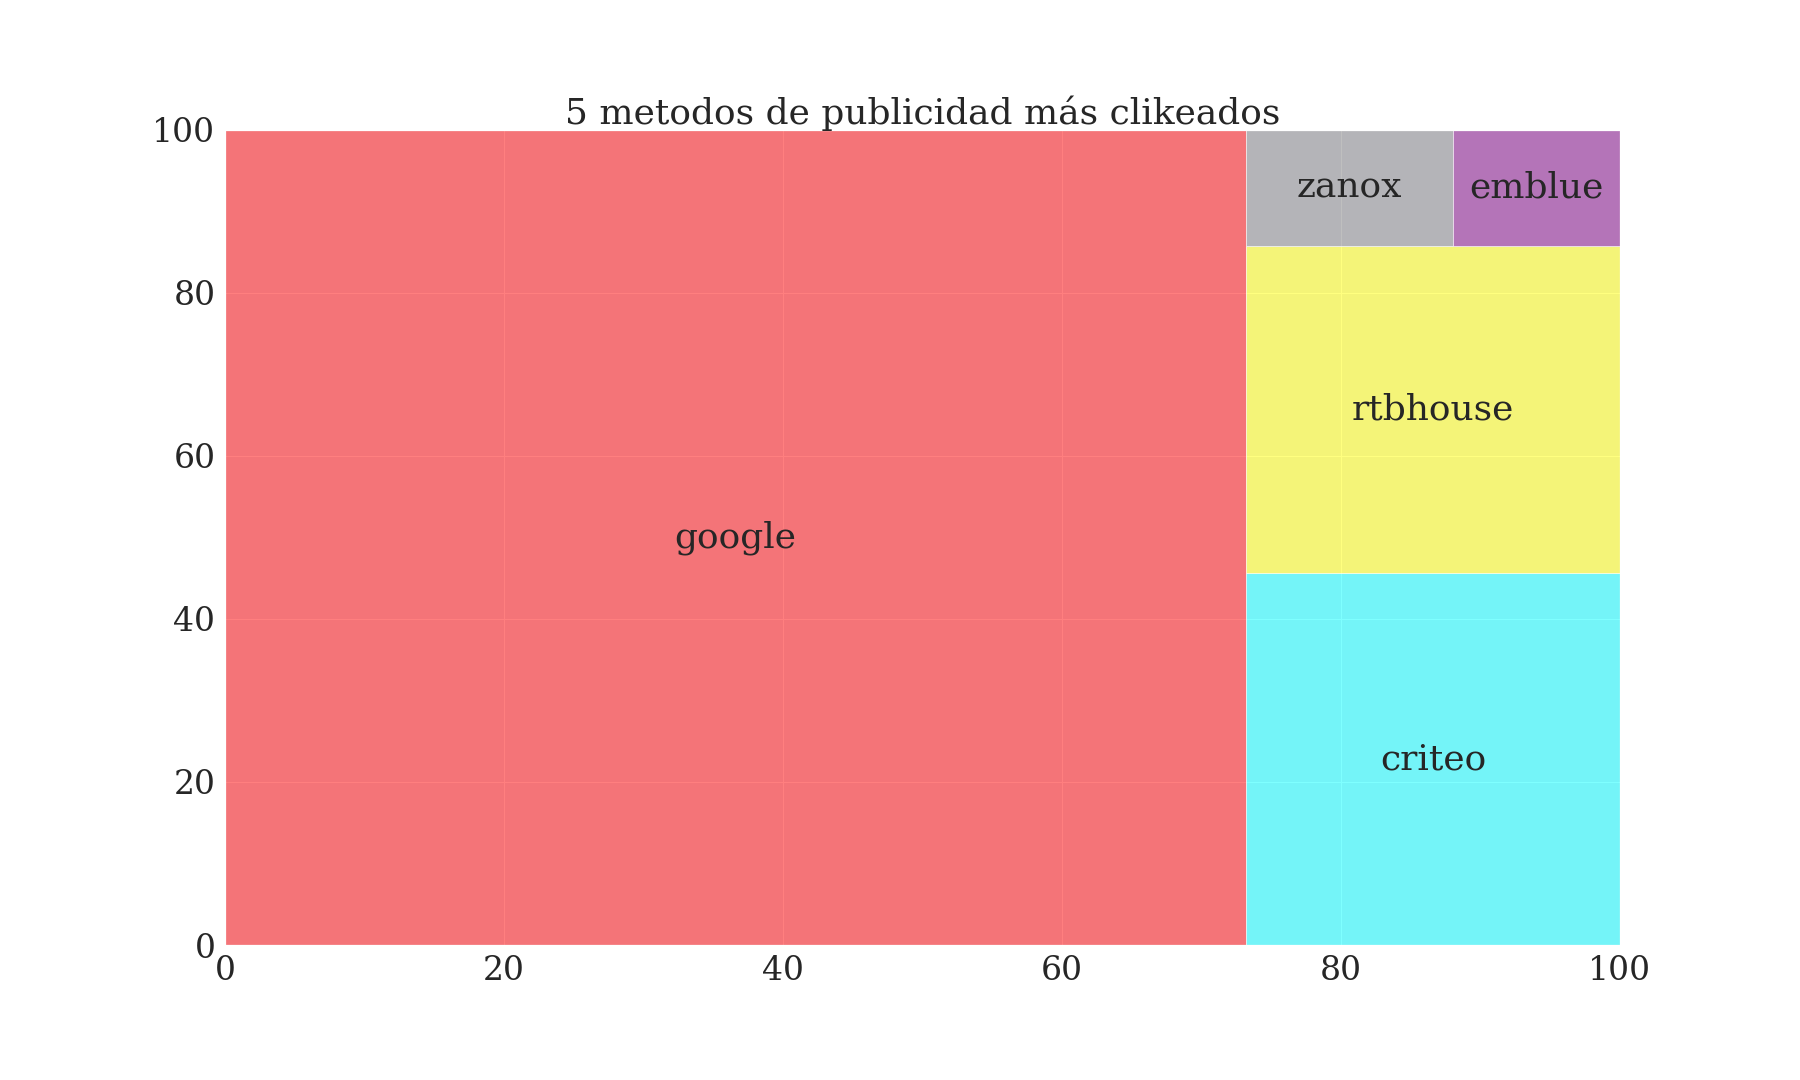
\includegraphics[width=\linewidth]{figures/170-publicidad_clickeada-barplot.png}
	\caption{Métodos de publicidad que generan visitas en Trocafone}
	\label{fig:metodopublicidad}
\end{figure}

\begin{figure}[!h]
	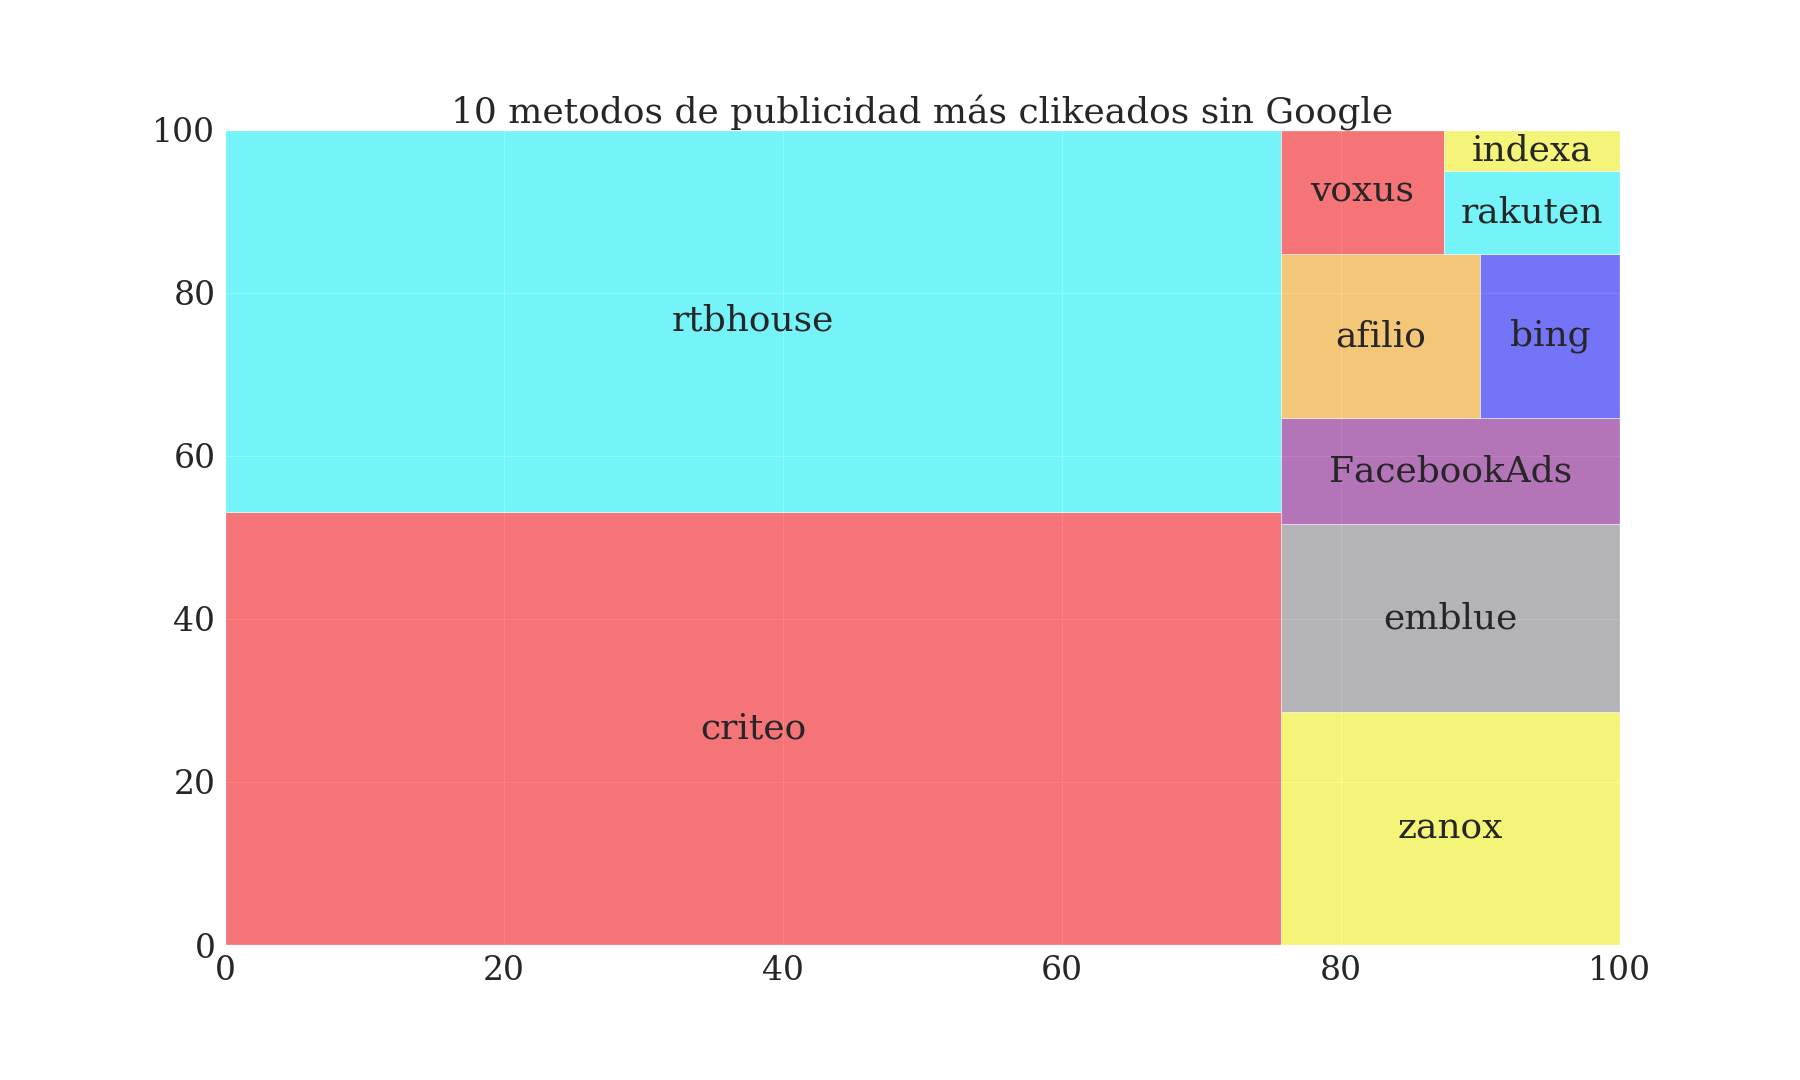
\includegraphics[width=\linewidth]{figures/171-publicidad_sin_google-barplot.png}
	\caption{Cantidad de eventos de acuerdo al dispositivo utilizado}
	\label{fig:metodopublicidadsingoogle}
\end{figure}

Se concluye de estos gráficos \ref{fig:metodopublicidad} y \ref{fig:metodopublicidadsingoogle} que el método de publicidad más eficiente es \textbf{Google}. Por lo tanto, es conveniente que \textbf{Trocafone} mantenga su contrato con el mismo para aumentar las visitas a su página. Los otros métodos de publicidad son efectivamente mucho menores y parecen no tener mucha relevancia para el tráfico del sitio. Es por esto que quizás sería necesario que \textbf{Trocafone} haga un balance entre los gastos consumidos y la ganancia obtenida con el uso de esos métodos publicitarios.

\subsection{Funnel por publicidad}

Habiendo obtenido las sesiones por usuario, se puede observar como se inicia cada una. Para esto se generó un \textit{funnel} que no solo indica la cantidad de tráfico por cada paso, sino que también muestra la proporción del mismo que proviene de una campaña publicitaria.

\begin{figure}[!h]
	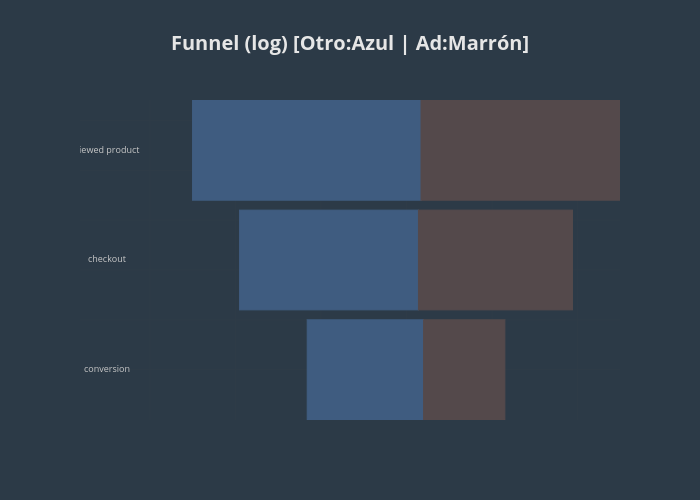
\includegraphics[width=\linewidth]{figures/200-advertisement-funnel.png}
	\caption{Funnel según provengan de campaña publicitaria}
	\label{fig:funnel}
\end{figure}

El gráfico \ref{fig:funnel} muestra que si bien casi la mitad del tráfico proviene de \textit{advertising} tanto para \textit{viewed product} como para \textit{checkout}, la razon cae mucho en la etapa de \textit{conversion}, donde menos de el 15\% del tráfico de esta fuente termina en una compra.

\section{Análisis de canales de tráfico}

Sabiendo que un usuario puede llegar desde diversos lugares, ver de dónde viene es algo muy importante para saber en que lugar debe la empresa invertir. ¿Debe tener mayor presencia en las redes sociales? ¿Debe invertir en su visibilidad online mediante procesos de SEO\footnote{Search engine optimization}? 

Lo que en particular nos interesa es la métrica llamada \textbf{revenue by traffic source}, la cual se refiere no a los usuarios que vienen, si no los usuarios que vienen y hacen una conversion (compra), como una manera de representar los métodos realmente efectivos (después de todo, la efectividad de la empresa radica en que un usuario haga una conversión, no meramente en que entre al sitio).

Los canales de tráfico presentes en el dataset son:
\begin{itemize}
\item \textbf{Paid: } Usuarios que llegan mediante una campaña de marketing.
\item \textbf{Direct: } Usuarios que llegan directamente al sitio, sin ayuda externa (por ejemplo, escribiendo directamente la url en el explorador web, un marcador, un link de un documento sin tracking)
\item \textbf{Email: } Usuarios que llegan desde un link en un email.
\item \textbf{Organic: } Usuarios que llegan desde motores de búsqueda.
\item \textbf{Referral: } Usuarios que llegan al sitio desde otro sitio web.
\item \textbf{Social: } Usuarios que llegan desde redes sociales.
\end{itemize}

\begin{figure}[!h]
	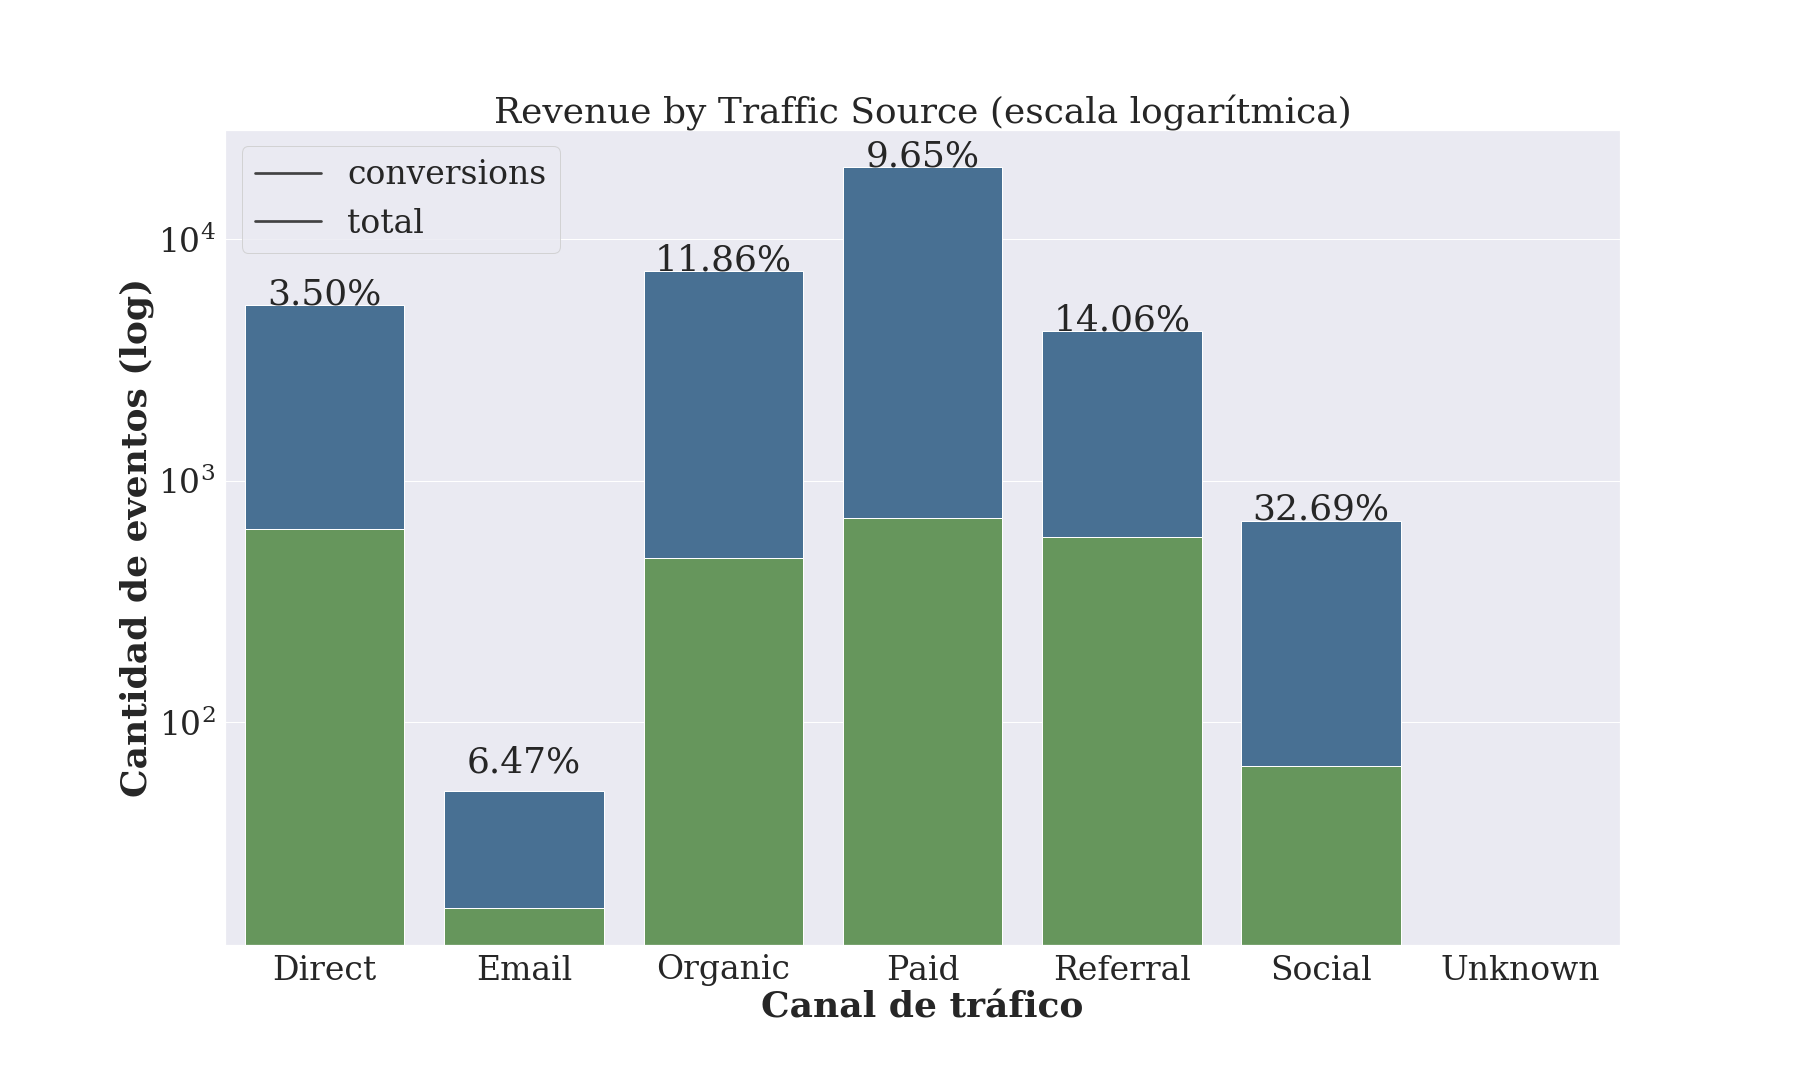
\includegraphics[width=\linewidth]{figures/180-revenue_traffic-boxplot.png}
	\caption{Canales de tráfico y sus ganancias}
	\label{fig:traffic}
\end{figure}

Lo que observamos en el gráfico \ref{fig:traffic} es que si bien el canal pago es el que más usuarios atrae, tiene una ganancia bastante razonable para la magnitud de usuarios que atrae. Por lo tanto seguir invirtiendo en él probablemente lleve a un retorno con incremento constante y no tan significante\footnote{Como ejemplo de la ley de los rendimientos decrecientes}.

Por otro lado son otros canales los que verdaderamente sorprenden por su porcentaje de retornos. Hay un gran retorno de parte de la presencia de las redes sociales, que puede no atraer tantos usuarios pero a los que atrae lo hace de manera muy efectiva, y lo mismo aplica para la presencia onlina organica de Trocafone, donde se ve que si se invirtiese en procesos de SEO esto podría llevar tanto a más usuarios como más compras.



\section{Conclusiones}

Antes de presentar las conclusiones obtenidas a partir del análisis del dataset presentado es necesario volver a remarcar que los datos no representan el total de datos de la empresa \textbf{Trocafone}. Se descubrió que los únicos datos presentados eran de clientes que habían realizado al menos un \texttt{checkout}, por lo que mínimamente se detecta un truncamiento allí. Cabe la posibilidad de que se haya truncado con algún otro criterio que no se haya detectado con el análisis presentado. Además, los datos corresponden a la página web de Trocafone, por lo que no constituye el total de datos de ventas de la empresa, que también se encargan de vender a otros proveedores.

Este recordatorio tan reiterado no deja de ser sumamente importante, de tener más datos (como por ejemplo un semestre en su totalidad, sin truncamientos) se podría hacer un análisis más a pleno, ni hablar de si se tuviesen más atributos, ya que una de las dificultades encontradas en el trabajo fue la falta de atributos numéricos, dependiendo solamente de contar valores (por ejemplo, un dato sumamente rico en información es el precio de venta, o poder decir más del usuario como su edad y/o sexo).

\subsection{Insights}

En primer lugar se considera que de la cantidad de conversiones detectada en el set de datos no puede extraerse alguna conclusión en cuanto a cuan bien o mal le fue a la empresa en el semestre, por falta de conocimiento y manejo del dominio (plataformas de e-commerce en el rubro de celulares). Otro lugar donde se ve la falta de dominio es en el no poder explicar la cantidad de registros de mayo (considerablemente mayor al resto de los meses). De tener mayor conocimiento del estado de Brasil (puede ser producto de política), de la industría de la tecnólogia celular (constantemente hay nuevos lanzamientos de celulares que incentivan vender el previamente usado, leyes que influyen tanto para bien como para mal la compra/venta y demás) o de \textbf{Trocafone} en sí (por ejemplo, un lanzamiento de descuentos o promociones) se tendrían más recursos para poder explicar lo que a simple vista parece una anomalía. En cambio, si se ha podido analizar en su lugar la comparación \textit{checkout vs conversiones vs viewed products} a lo largo de diferentes parámetros como marcas de celulares o períodos de tiempo, mostrando como el sitio web cumple o no su objetivo de mantener a los usuarios y hacerlos comprar por allí.

Del análisis de la cantidad de eventos mencionados previamente en función de las marcas de celulares se concluye que las marcas que tienen un precio más accesible como lo puede ser \textbf{Samsung} eran de las menos vistas pero de las más compradas. Asímismo, las marcas con un precio más elevado como \textbf{Apple} eran de las más vistas pero de las menos compradas. Esta era una situación prevista de antemano debido a que la calidad del producto de mayor precio atrae visitas pero su precio aleja las compras. Asímismo, un celular de menor precio y calidad es más probable que si es visto sea comprado por el mismo usuario debido a que la calidad del producto no suele atraer visitas que no sean potenciales compradoras en un futuro. 

También se observa que no tiene sentido seguir comerciando algunos productos, por ejemplo los \textbf{Blackberry}, \textbf{Quantum} y  \textbf{iPad}, ya que se necesita disponer de expertos para repararlos que no son justificados por la cantidad de conversiones que tienen. De todas formas, sacarle la posibilidad de vender y reacondicionar su celular usado a un futuro cliente no sería una buena estrategia de negocio.

Un análisis similar puede realizarse en cuanto al sistema operativo del cual proviene el que genera una compra y el sistema operativo del dispositivo comprado. Los usuarios que provienen de \textbf{Apple} suelen desear comprar un dispositivo del mismo sistema operativo debido a su calidad y al atractivo que suelen manejar los productos de \textbf{Apple} en la sociedad. De otra manera, los usuarios que provienen de \textbf{Android} divergen sus visitas en cuanto al sistema operativo ya que no se detecta un comportamiento específico para este tipo de usuarios.

\subsection{Aportes a Trocafone}

Teniendo en cuenta lo descubierto en el trabajo, se propone:

\begin{itemize}
\item \textbf{Publicidad en horarios pico y promociones en horarios con menor tráfico.} Teniendo en cuenta los horarios de menor y mayor tráfico como las 19hs (la hora del día que se registran más checkouts y conversiones), se podría agregar publicidad que incentive el aumento de tráfico y promueva la realización de conversiones. Así mismo, los días que se registra menos tráfico como los fines de semana o el horario del mediodía podría agregarse alguna promoción para aumentar la cantidad de eventos en dichos horarios y expandir la franja horaria de tráfico en la página.

\item \textbf{Optimizar las páginas estaticas de soporte.} En lo que respecta a páginas estáticas, se llegó a la conclusión de que una buena inversión de parte de la empresa sería optimizar el sitio de preguntas frecuentes, ya que se notó que hay una gran cantidad de tráfico a \textit{customer service} que podría redirigirse a las \textit{FAQ} para optimizar el uso del personal en responder en atencion al cliente y que los usuarios encuentren rápidamente respuestas a sus preguntas específicas.

\item \textbf{Optimizar el sitio de entrada.} Se observó que la tasa de usuarios que ingresa solo una vez es mucho mayor que la de usuarios que regresan. Si bien este es un problema con el que todo sitio se encuentra, una forma de disminuir lo más posible la diferencia puede ser mejorar la experiencia de usuario en el sitio de entrada.

\item \textbf{Presencia online.} Una sugerencia en cuanto a inversión en presencia online esta tanto en los motores de busqueda como en las redes sociales. Ambos canales de tráfico tienen un potencial muy grande en cuanto a atraer usuarios que efectuan conversiones, e invertir en ellos lograría mantener el porcentaje de efectividad mientras se incrementa el número total de usuarios atraídos.

\item \textbf{Utilizar los productos más comprados como lideres en la publicidad.}  Podría aprovecharse el conocimiento sobre los productos más visitados para encarar con su imagen las publicidades, logrando así nuevas visitas a la página y con ellas, nuevas posibilidades de ventas. Una vez que el cliente se encuentre dentro de la plataforma virtual se puede utilizar el conocimiento sobre los productos más vendidos y dar fácil acceso a su publicación. La lista presentada en la tabla \ref{table:modelos_prominentes} es representativa tanto de los modelos más codiciados como los modelos más comprados.

\item \textbf{Texto predictivo y autocompletar las busquedas.} Viendo en la figura \ref{fig:searchedterm} los términos más buscados por usuarios en crudo (es decir, sin modificación), se nota que hay varios usuarios que no encuentran de entrada lo que buscan, con varios errores de tipografía y demás. Esto hace que el usuario pase por un sitio intermedio (yendo desde su busqueda, hasta la lista de dispositivos que encuentra, hasta el dispositivio que verdaderamente buscaba). Una forma de solucionar esto sería el autocompletar la busqueda por el usuario, haciendo que si escribe el nombre parcial de un modelo ya se le empiece a mostrar la lista de modelos que contienen ese texto, así salteando el sitio intermedio y yendo directamente de la busqueda a visitar el producto. 

\item \textbf{Calidad de la publicidad.} Teniendo en cuenta que casi la mitad de las sesiones se generan debido a la publicidad, pero que sólo el 12.5\% de las sesiones que terminan en una conversión provienen de esta, se tiene que considerar que debería mejorarse la calidad de la misma, y no tanto la cantidad, mostrándole al usuario un producto más acorde a su perfil, por ejemplo, a un usuario de iOS se le ofrecería un iPhone como publicidad (apoyandonos en el gráfico \ref{fig:sankey} de fidelidad), mejorando así las chances de conversión.

\end{itemize}

\newpage
\appendix

\section{Ejecución}

El trabajo fue realizado en Anaconda\footnote{\url{https://anaconda.org/}}. Para poder replicar el trabajo, hay que también instalar las siguientes librerías adicionales:

\begin{itemize}
	\item{Squarify\footnote{\url{https://github.com/laserson/squarify}}: Para los treemaps.}
	\item{pySankey\footnote{\url{https://github.com/anazalea/pySankey/}}: Para los diagramas de Sankey (diagramas de flujo).}
	\item{Plotly\footnote{\url{https://plot.ly/}}: Para poder graficar las sesiones de usuario. Su módulo \texttt{Orca} sirve para exportas las imagenes estáticas.}
	\item{Geopandas\footnote{\url{http://geopandas.org/}}: Para poder graficar sobre mapas geográficos.}
	\item{Wordcloud\footnote{\url{https://github.com/amueller/word_cloud/}}: Para poder visualizar los términos más buscados.}
\end{itemize}

Estos pueden ser instalados con los siguientes comandos (se incluyen los comandos de \texttt{conda} cuando sea posible): 
\begin{lstlisting}[language=sh]
pip install squarify
pip install pySankey
conda install -c plotly
conda install -c plotly plotly-orca
conda install -c conda-forge geopandas
conda install -c conda-forge wordcloud
\end{lstlisting}

Alternativamente, se puede optar por correr el código sobre el kernel publicado en la plataforma Kaggle.

\section{Datasets adicionales incoporados para el análisis}

Se utiliza adicionalmente un dataset del mapa de Brasil y sus ciudades, para el análisis geográfico. Este fue sacado de  Geonames\footnote{\url{http://www.geonames.org/}}, una base de datos publica de paises y regiones del mundo.

\end{document}